% DOCX paragraph 828
\chapter{La primera imagen de un agujero negro}\label{ch:07}

% DOCX paragraph 829

% DOCX paragraph 832
Hasta aquí hemos estudiado en detalle las propiedades de los agujeros negros y los desafíos intelectuales que plantean. Ha llegado el momento de presentar un logro científico reciente de gran importancia, en el que he tenido la fortuna y el privilegio de participar como uno de los 13 miembros del Comité Ejecutivo de la colaboración Event Horizon Telescope\index{Event Horizon Telescope} (EHT).

% DOCX paragraph 833
\begin{figure}[htbp]
\centering
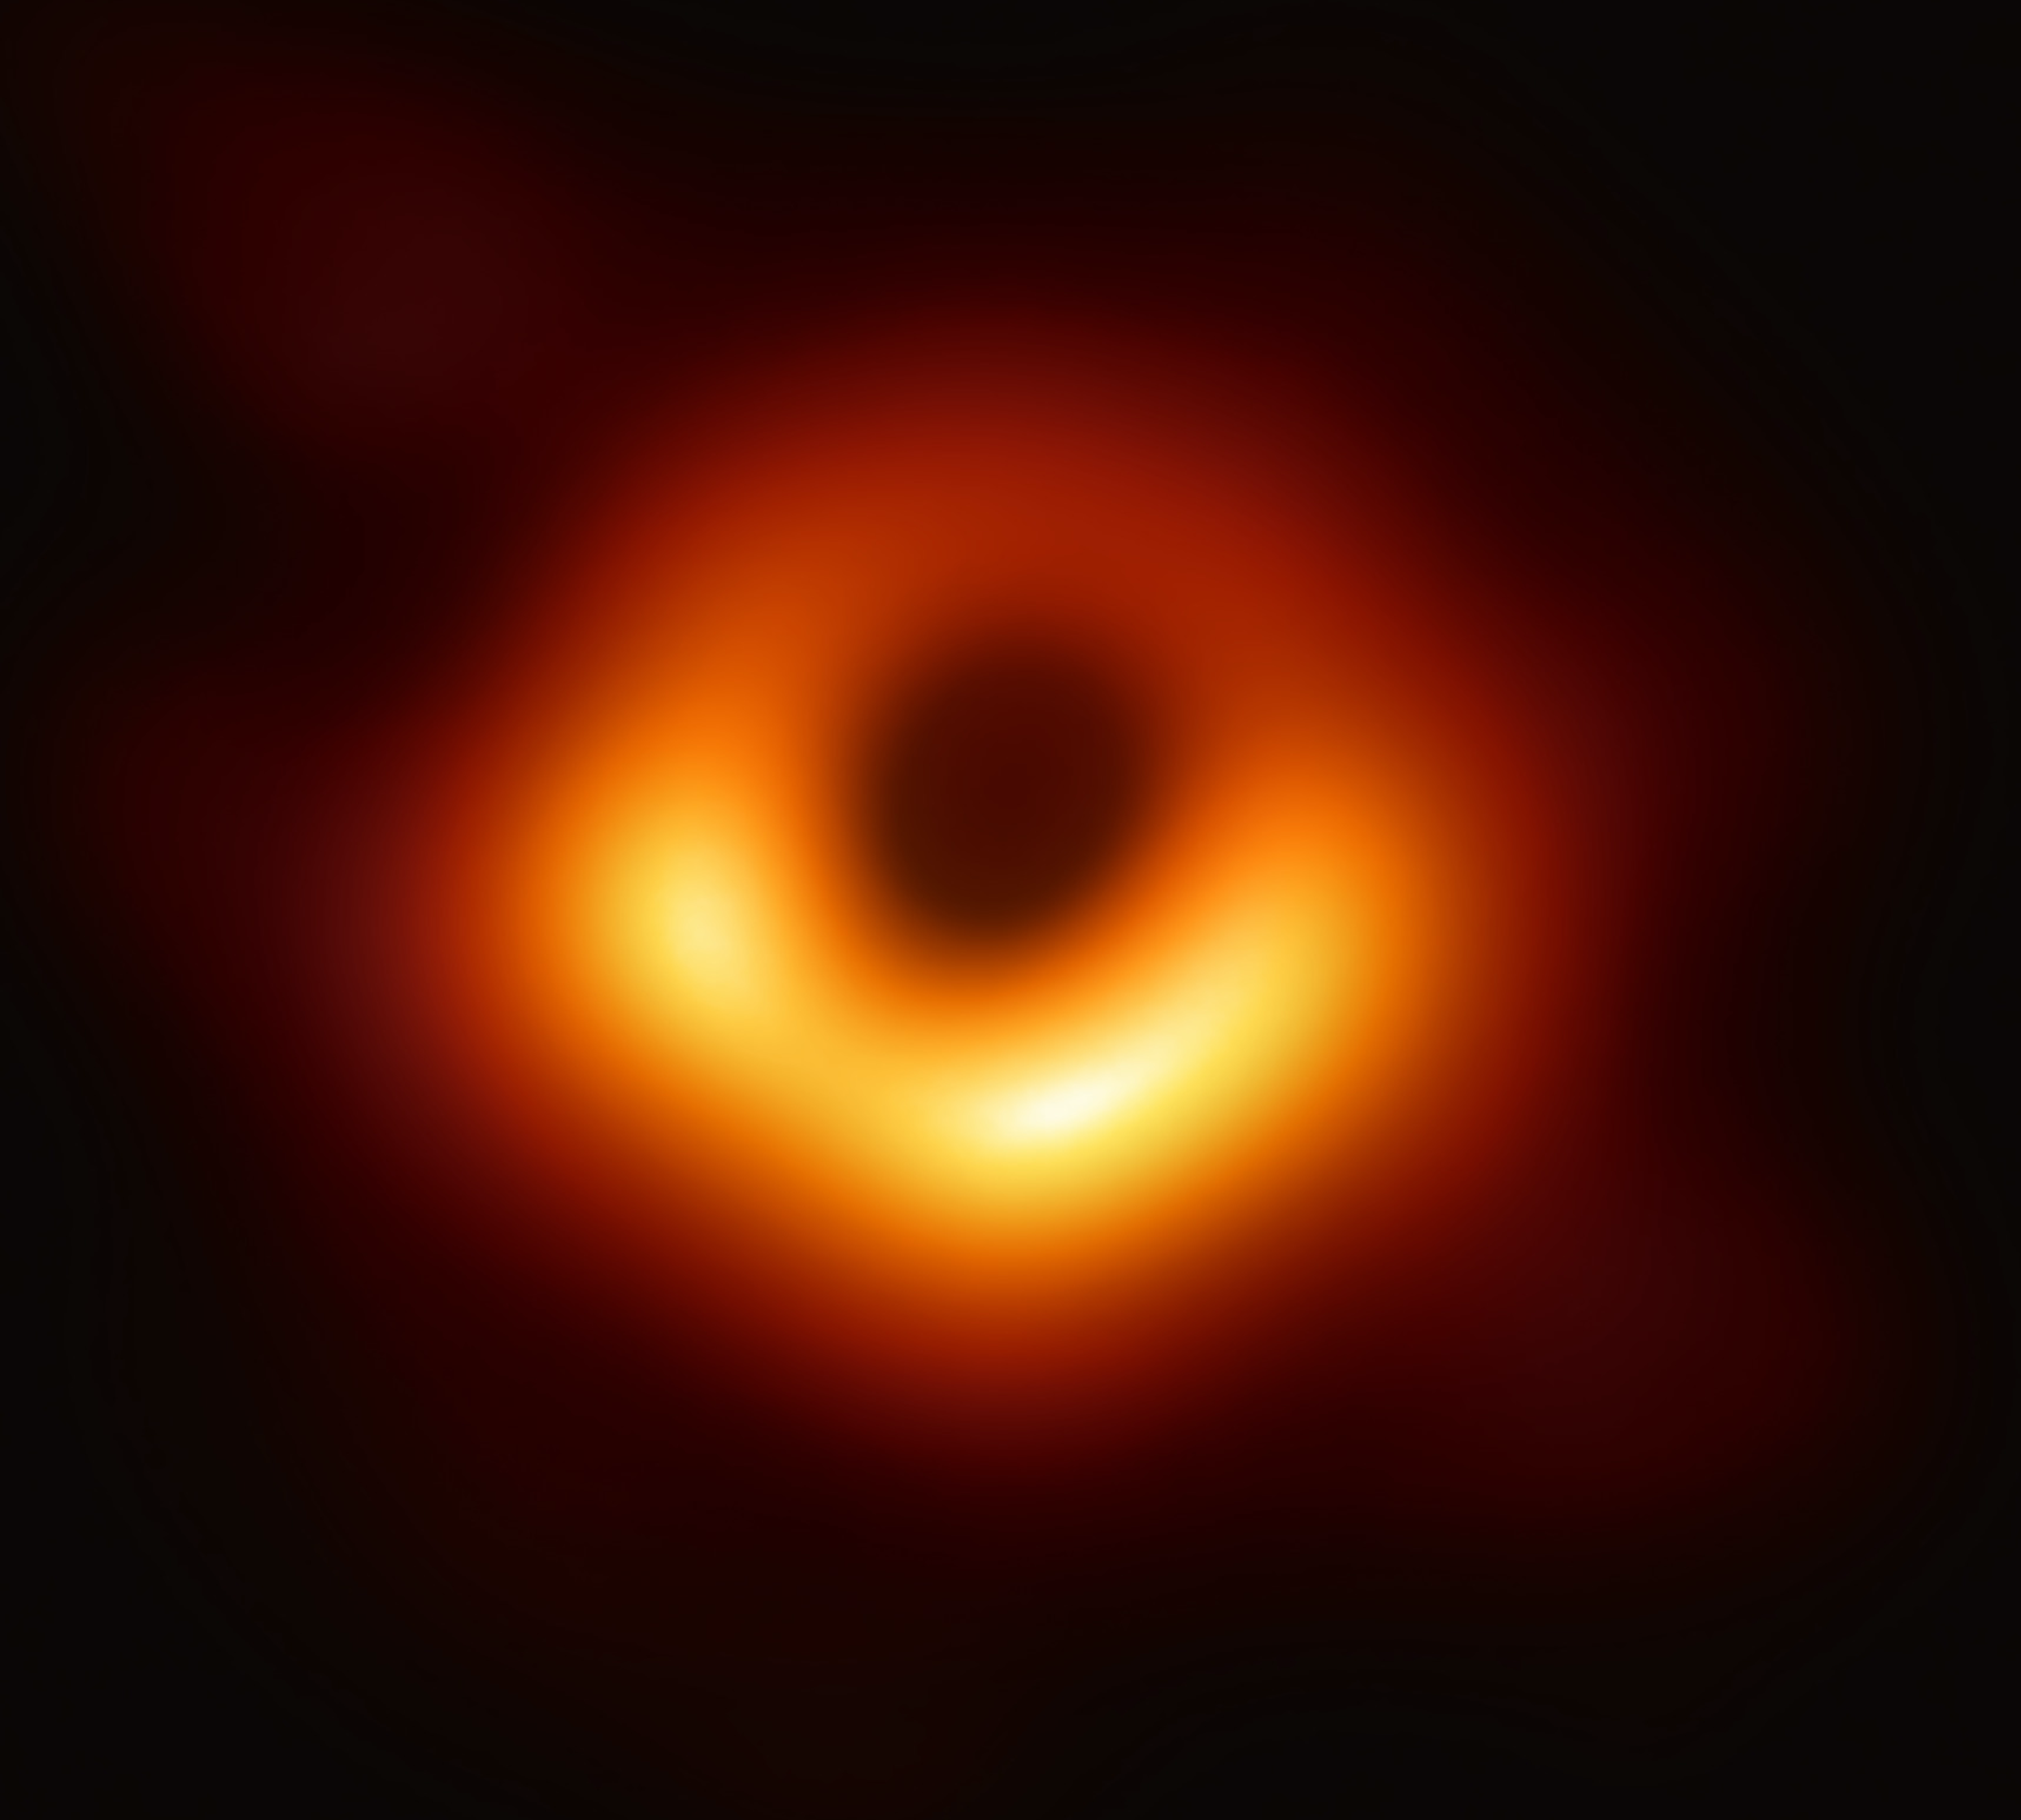
\includegraphics[width=0.88\linewidth,height=0.48\textheight,keepaspectratio]{../figs/pdf/en/fig-07-01.pdf}

% DOCX paragraph 835
\caption{\emph{Imagen de radio de M87\textsuperscript{*}, a una longitud de onda de 1,3 mm. © The EHT Collaboration.\index{M87*}}}\label{fig:07-01}
\end{figure}

% DOCX paragraph 837
Este capítulo está dedicado a la realización de la primera imagen de un agujero negro supermasivo: M87\textsuperscript{*}, situado en el centro de la galaxia elíptica de la que toma su nombre, Messier-87, o simplemente M87.\index{M87*}

% DOCX paragraph 838
A menos que hayas pasado los últimos años en otro planeta o en una cueva aislada, es poco probable que no hayas visto ya la imagen de la figura \ref{fig:07-01}, publicada por la colaboración EHT el 10 de abril de 2019. Se estima que, en las primeras 24 horas, la vieron 4\,500 millones de personas. Desde entonces se ha convertido casi en un icono y en una fuente inagotable de comentarios e inspiración en las redes sociales. En menos de dos días, la inmensa mayoría de la población humana había visto la imagen: un récord difícil de batir. Incluso hoy, más de dos años después, sociólogos y filósofos se preguntan por qué la imagen de media rosquilla luminosa ha despertado tanto interés y se ha convertido en la foto del siglo, merecedora de un lugar en el Museo de Arte Moderno, el MoMA, de Nueva York.

% DOCX paragraph 839
Dada su popularidad, es posible que ya sepas cómo se obtuvo esta imagen y por qué creemos que inmortaliza un agujero negro supermasivo. Si no es así, no te preocupes: en las páginas siguientes te guiaré para que la comprendas mejor. Veremos cómo se produjo y cómo la comparación entre las observaciones y la teoría nos ha llevado a concluir que se trata, en efecto, de un agujero negro.

% DOCX paragraph 840
Pero antes conviene despejar el terreno de algunas especulaciones que surgieron poco después de publicarse la imagen. Se ha afirmado que lo que aparece en la figura \ref{fig:07-01} no es una auténtica «foto», sino un mapa de la emisión de radio de M87*\index{M87*}.

% DOCX paragraph 841
Personalmente, estas consideraciones me parecen bastante pedantes. Para que quede claro: quienes afirman que la figura \ref{fig:07-01} es un mapa de radio transformado en una imagen tienen toda la razón. Pero no olvidemos que todas las fotos son el resultado de un proceso de cartografiado. Esto vale para las antiguas placas fotográficas, en las que la imagen se reconstruía mediante las distintas intensidades de luz a las que se exponía una emulsión de sales de plata. Y también para los selfis que tomamos con el móvil: la intensidad del campo eléctrico registrada por un sensor situado detrás de la lente se transforma en una foto nuestra frente al Coliseo. Incluso vale para lo que ves ahora mismo mientras lees este texto. La imagen del mundo que percibes no es más que un mapa de la distribución de energía de los fotones que inciden en las células fotosensibles situadas en la parte posterior de la córnea, transmitido a través de una densa red de nervios e interpretado después por el cerebro.\index{foton@fotón}

% DOCX paragraph 842
Lo que quiero subrayar es que no existe una foto «real»: todo lo que vemos es el resultado de cartografiar las señales recibidas y procesarlas para formar una imagen. Y aunque nuestros ojos no son sensibles a la banda de radio, eso no significa que no podamos obtener una foto a partir de esa radiación. Sería como decir que las imágenes de nuestros hijos cuando aún estaban en el vientre materno, que muchos conservamos, no son «fotos» porque nuestros ojos no son sensibles a la radiación en la banda de ultrasonidos. Espero que lo absurdo de esa afirmación resulte evidente.

% DOCX paragraph 843
En conclusión, a todos los efectos prácticos, la imagen de la figura \ref{fig:07-01} es la primera foto de un agujero negro supermasivo, obtenida por la colaboración EHT. Que se haya producido a partir de una medida de radio a frecuencias a las que no somos sensibles es un detalle completamente irrelevante.

% DOCX paragraph 847
\section{Hacer lo que se creía imposible}\label{sec:07-impossible}

% DOCX paragraph 849
Permíteme comenzar con una pregunta tan obvia como habitual: «¿Cómo es posible fotografiar un horizonte de sucesos\index{horizonte de sucesos} si, por definición, no puede emitir luz?». La respuesta es sencilla y categórica: ¡no se puede! Fotografiar un objeto significa recoger los fotones que emite, pero el horizonte de sucesos, por definición, no emite fotones y es, por tanto, «invisible» para un observador exterior. Dicho esto, sí es posible fotografiar lo que está cerca y alrededor del horizonte, sobre todo si lo rodea un plasma\index{plasma} caliente que cae sobre él y emite radiación\textsuperscript{\hyperlink{note:07-01}{1}}. Eso es exactamente lo que hicimos en la colaboración EHT y lo que interesa a los astrofísicos.

% DOCX paragraph 850
Es evidente que fotografiar lo que está cerca de un agujero negro no demuestra su existencia. Pero supongamos que la imagen observada coincide con las predicciones teóricas basadas en la dinámica del plasma\index{plasma} cerca de un horizonte de sucesos. Entonces tenemos pruebas convincentes de que hay un agujero negro. Dicho de otro modo, la foto obtenida coincide con la imagen que produciría un agujero negro supermasivo si nos acercáramos lo suficiente.

% DOCX paragraph 851
Estas consideraciones conducen inevitablemente a otra pregunta: «Si es imposible fotografiar el horizonte de sucesos, pero podemos obtener una imagen de lo que hay a su alrededor, ¿por qué no se ha hecho antes?». La respuesta se deduce de lo que hemos aprendido sobre las propiedades de los agujeros negros. Hemos visto que son los objetos más compactos del universo, hasta el punto de que, si quisiéramos producir uno a partir del Sol, tendríamos que reducir el radio de nuestra estrella a no más de 3 kilómetros. Es fácil comprender lo difícil que sería observar un objeto celeste de solo 3 kilómetros de radio a distancias astronómicas, es decir, mucho más allá del sistema solar.

% DOCX paragraph 852
Dejando de lado que solo una pequeña parte de la emisión de un agujero negro situado a distancias astronómicas puede alcanzarnos, el problema más grave para observarlo es la resolución\index{resolución|see{resolución angular}} angular\index{resolución angular}. Es decir, la posibilidad de utilizar un telescopio, o un conjunto de telescopios, con nitidez suficiente para distinguir un objeto de tamaño muy pequeño en el cielo. Veamos algunos números. Un agujero negro de masa estelar muy cercano, digamos a un millón de unidades astronómicas, o UA, equivalentes a un millón de veces la distancia entre la Tierra y el Sol, tendría un tamaño angular proyectado en el cielo de 10\textsuperscript{--10} segundos de arco, o 0,0001 microsegundos de arco, es decir, aproximadamente 3 × 10\textsuperscript{--14} grados. A modo de ilustración, esta resolución permitiría a alguien situado en Roma distinguir un objeto del tamaño de un grano de arroz en Nueva York. No existe ningún telescopio, ni conjunto de telescopios, capaz de alcanzar esa resolución angular, ni siquiera con la tecnología más avanzada. Como veremos, la mejor resolución a la que podemos aspirar es del orden de decenas de microsegundos de arco, y eso ya sería toda una proeza tecnológica.\index{UA (unidad astronómica)}

% DOCX paragraph 853
Por tanto, si queremos fotografiar un agujero negro, debemos descartar los estelares: son demasiado pequeños para verlos a distancias astronómicas. Como el tamaño aumenta con la masa (recuerda la expresión del radio de Schwarzschild...), nos quedan los agujeros negros supermasivos. Cuanto más masivos, mejor, pues a una distancia dada parecerán mayores. La distancia también cuenta: como ocurre con cualquier objeto, cuanto más lejos esté el agujero negro, más pequeño aparecerá en el cielo, incluso si su masa es enorme. Así pues, los «requisitos» para los candidatos ideales en este concurso de fotografía son tener una masa enorme y estar lo bastante cerca.

% DOCX paragraph 854
Una vez aplicados estos dos «filtros de selección» a los cientos de miles de agujeros negros supermasivos que creemos conocer en el universo, solo quedan dos candidatos de interés. Son agujeros negros para los que un tamaño proyectado de unos diez microsegundos de arco corresponde a un tamaño físico de unos 10 radios de Schwarzschild.

% DOCX paragraph 855
Los dos candidatos que siguen en el concurso son Sagitario A\textsuperscript{*}, o simplemente Sgr A\textsuperscript{*}, el agujero negro del centro de nuestra galaxia, y M87\textsuperscript{*}. El primero interesa porque, como puedes imaginar, es el más cercano: lo que le falta en masa lo compensa con su proximidad, ya que tiene «solo» unos pocos millones de masas solares. El segundo está más lejos, de hecho mil veces más lejos, pero lo compensa con su masa: es casi mil veces más masivo que Sgr A* y figura entre los agujeros negros más masivos que conocemos.\index{Sagitario A* (Sgr A*)}\index{M87*}

% DOCX paragraph 856
Ahora que hemos elegido a nuestros candidatos ideales, vayamos a la caza de estos agujeros negros...

% DOCX paragraph 859
\section{Un telescopio del tamaño de la Tierra}\label{sec:07-telescope}

% DOCX paragraph 861
Para comprender cómo se obtuvo la imagen de la figura \ref{fig:07-01}, primero debemos ocuparnos de los aspectos técnicos y tecnológicos de las observaciones. Por eso, y para apreciar hasta qué punto las matemáticas están en el origen de toda comprensión física, déjame mostrarte la siguiente ecuación conceptual, muy general y fácil de entender:

% DOCX paragraph 863
\begin{equation}\label{eq:07-01}
\begin{pmatrix}\text{resolución angular de la} \\ \text{imagen astronómica}\end{pmatrix}
=\left(\frac{\text{longitud de onda de las observaciones}}{\text{tamaño del telescopio}}\right)
\end{equation}

% DOCX paragraph 864

% DOCX paragraph 866
La ecuación \eqref{eq:07-01} nos dice que, si queremos obtener una resolución angular\index{resolución angular} muy pequeña, para distinguir detalles diminutos y estudiar objetos cuyo tamaño proyectado en el cielo es muy pequeño, debemos procurar que la razón entre la longitud de onda de las observaciones y el tamaño del telescopio sea lo menor posible.

% DOCX paragraph 867
Podrías pensar que la forma más sencilla de reducir ese cociente sería observar a las longitudes de onda más cortas, es decir, en la banda de rayos X o incluso de rayos gamma\index{rayos gamma|see{astronomía}}\index{radiación!rayos gamma}. Por desgracia, no es una opción: sencillamente, no recibimos ni podemos recibir radiación\index{rayos X!radiación} de rayos X o gamma de un agujero negro supermasivo. Para entender por qué, debemos distinguir entre la radiación\index{rayos X!radiación} emitida y la que llega a nuestros telescopios.

% DOCX paragraph 868
Un agujero negro supermasivo que acreta materia de su entorno emite radiación electromagnética\index{radiación!electromagnética} en un espectro\index{espectro!electromagnético} muy amplio. Además, como vimos para Cyg-X1, esa radiación es muy intensa en las bandas de rayos X y gamma. Estas emisiones se generan muy cerca del horizonte de sucesos, precisamente la región que más nos interesa observar. Pero la emisión de radiación es una condición necesaria y no suficiente para que una observación astronómica tenga éxito: también necesitamos que llegue hasta nuestros telescopios. Por desgracia, esto no ocurre en las bandas de rayos X y gamma, ni en la óptica. La razón es que hay bastante materia entre nosotros y la fuente, bien como plasma en acreción\index{plasma!en acreción} en condiciones extremas de temperatura y energía, bien como simple polvo interestelar. En ambos casos, esa materia absorbe muy eficazmente la radiación antes de que pueda alcanzarnos. Por eso, aunque el material que se acumula alrededor de un agujero negro supermasivo emite luz en un espectro\index{espectro!electromagnético} muy amplio, gran parte de ella se absorbe o se dispersa y nunca llega a nuestros telescopios.

% DOCX paragraph 869
Para explicar mejor la absorción y la dispersión, recurriré a una analogía. Pensemos en el cielo de un día nublado: si la cobertura no es muy densa y solo hay un velo de nubes, aún podemos ver la silueta del Sol como una mancha más luminosa en el cielo. Pero si las nubes forman una capa muy densa, nuestra estrella favorita no será visible, pues absorberán su radiación y esta no nos llegará, al menos directamente. Sin embargo, la luz solar sí nos alcanza en un día nublado: un día nublado no es tan oscuro como la noche. Esto ocurre porque las moléculas de vapor de agua\index{vapor de agua} de las nubes dispersan una y otra vez los fotones emitidos por el Sol, dando lugar a la luminosidad sin sombras de un día gris.

% DOCX paragraph 870
Volvamos a la ecuación \eqref{eq:07-01}. Para decidir qué longitud de onda emplear y qué resolución podemos esperar, debemos recurrir, no a la menor longitud de onda emitida, sino a la menor que puede recibirse en la Tierra. Dejando de lado los detalles de un modelo completo de la radiación\index{rayos X!radiación} emitida cerca de un agujero negro, la longitud de onda óptima para obtener la imagen de un agujero negro supermasivo está en la \emph{banda de radio} y es del orden de 1,3 milímetros, correspondiente a una frecuencia de unos 230 GHz. Esta longitud de onda es un millón de veces mayor que la de los rayos X, que ronda un nanómetro, pero tiene la ventaja de que el plasma que rodea al agujero negro es casi transparente a ella. Así, la radiación puede llegar hasta nosotros sin ser absorbida ni dispersada por el camino.

% DOCX paragraph 871
Una vez establecido que debemos recoger radiación en la banda de radio, nos queda un problema mucho más difícil: ¡recogerla! Necesitamos un radiotelescopio lo bastante grande como para alcanzar una resolución de unas decenas de microsegundos de arco. Por suerte, se pueden construir radiotelescopios de tamaño considerable, pues básicamente son estructuras de acero parecidas a enormes antenas parabólicas de televisión. Aunque la mayoría tiene diámetros de entre 20 y 50 metros, hay dos mucho mayores: el radiotelescopio del Observatorio de Arecibo\index{radiotelescopio!Arecibo}, en Puerto Rico, y el telescopio FAST\index{radiotelescopio!FAST}, en China, con un diámetro de 500 metros. Por desgracia, ni siquiera un radiotelescopio tan enorme alcanzaría la resolución que necesitamos: ¡se quedaría corto en al menos cinco órdenes de magnitud! Si usaras la ecuación \eqref{eq:07-01} para calcular el tamaño necesario para obtener una resolución de unos diez microsegundos de arco a una longitud de onda de un milímetro, descubrirías que hace falta un telescopio de unos 10\,000 kilómetros de diámetro. ¡Un telescopio del tamaño del planeta entero!

% DOCX paragraph 872
Puede parecer una hazaña imposible, pero el ingenio humano nos ha permitido utilizar todo el planeta como un telescopio. Para ello se desarrolló en la década de 1980 una técnica radioastronómica hoy muy extendida: la interferometría de muy larga base, o VLBI\index{VLBI (interferometría de muy larga base)}, por sus siglas en inglés.

% DOCX paragraph 878
\section{Una técnica deslumbrante}\label{sec:07-vlbi}

% DOCX paragraph 880
Podemos evitar aquí los detalles de la técnica VLBI, algunos bastante sofisticados. Basta recordar que la interferometría aprovecha la propiedad de «superposición lineal» de los fenómenos ondulatorios, ya sean ondas electromagnéticas\index{ondas!electromagneticas@electromagnéticas}, sonoras\index{ondas!sonoras} o sísmicas\index{ondas!sísmicas}. Esta propiedad permite combinar las ondas en lo que llamamos interferencia\index{interferencia}\index{ondas!interferencia}. La interferencia es constructiva\index{interferencia!constructiva} cuando las amplitudes se suman y destructiva\index{interferencia!destructiva} en el caso contrario. La técnica VLBI está diseñada para aprovechar la interferencia entre las señales recibidas por dos radiotelescopios separados por miles de kilómetros, como el de Pico Veleta\index{radiotelescopio!Pico Veleta}, en España, y el telescopio ALMA\index{radiotelescopio!ALMA (Atacama Large Millimeter Array)}, en Chile. Es como si hubiéramos construido un único radiotelescopio \emph{virtual} cuyo diámetro fuera igual a la distancia entre los dos radiotelescopios \emph{reales}.

% DOCX paragraph 881
La técnica VLBI es realmente asombrosa, hasta el punto de parecer demasiado buena para ser verdad y hacernos preguntar: «¿Dónde está el truco?». No hay ningún truco, claro, pero sí unas restricciones precisas, algunas bastante severas.

% DOCX paragraph 882
La primera es garantizar que ambos radiotelescopios observen el mismo objeto en el mismo instante. La razón es bastante obvia: sin una sincronización perfecta, no tendríamos la certeza de que miden el mismo frente de onda de la radiación electromagnética\index{radiación!electromagnética}. Esto invalidaría todo el proceso interferométrico y las observaciones no darían lugar a una imagen.

% DOCX paragraph 883
Recuerda que la luz se propaga como una onda y que los frentes de onda emitidos por fuentes situadas a distancias astronómicas llegan a la Tierra como frentes planos y paralelos. Para garantizar que dos telescopios registren el mismo frente de onda, la lectura del campo eléctrico medida por el receptor de radio (incluso una radio doméstica registra un campo eléctrico que varía con el tiempo) debe combinarse con la lectura del instante en que llega ese frente. Por eso, cada telescopio debe estar equipado con un reloj atómico\index{atómico!reloj} de enorme precisión que marque el momento de llegada de la señal eléctrica.

% DOCX paragraph 884
La segunda restricción de la técnica VLBI es que la imagen no se puede producir en tiempo real, sino solo después de correlacionar las señales de dos o más telescopios. Por eso, cada observación, que ya genera cantidades enormes de datos, del orden de cientos de terabytes, debe registrarse y enviarse a un centro especial de supercomputación, donde se combinan los distintos flujos de datos para realizar la interferometría entre los telescopios. Para complicar aún más las cosas, resulta casi imposible transferir esos datos por internet, pues los radiotelescopios están donde la visibilidad es óptima, a menudo en lugares aislados y de difícil acceso: ¡uno de los telescopios del EHT está en el Polo Sur! Suelen construirse en zonas extremadamente áridas, ya que el vapor de agua\index{vapor de agua} es el mayor enemigo de las observaciones de radio. Por eso, una vez registrados en soportes físicos, los datos deben transportarse al centro de supercomputación encargado de combinarlos, normalmente con estudiantes que hacen de mensajeros.

% DOCX paragraph 885
Estos detalles deberían darte una primera idea de las complicaciones tecnológicas asociadas a la técnica VLBI y mostrar, al menos en parte, lo difícil que resulta utilizarla en la práctica. Sin embargo, el EHT ha elevado aún más el listón de esa sofisticación tecnológica en al menos dos aspectos. El primero es el número de radiotelescopios empleados. El principio de funcionamiento entre dos telescopios puede extenderse a una red entera, en la que cada instrumento se conecta individualmente con todos los demás. Esto aporta dos ventajas importantes: mejora la calidad de la imagen y prolonga el tiempo de observación. Con solo dos radiotelescopios, la imagen interferométrica es aproximada y contiene únicamente los rasgos básicos principales. Conviene, por tanto, utilizar tantos radiotelescopios como sea posible para mejorarla y obtener más detalles. Además de aportar información, disponer de más radiotelescopios permite «seguir» la fuente durante más tiempo. Cuando la rotación de la Tierra hace que desaparezca bajo el horizonte de uno de ellos, otros todavía pueden detectarla, pues acaba de aparecer en su cielo. Por ejemplo, en un día dado, el radiotelescopio de Pico Veleta, en España, será el primero en registrar una fuente como M87*\index{M87*}, mientras que el telescopio JCMT\index{radiotelescopio!JCMT (James Clerk Maxwell)}, en Hawái, será el último. Con ocho radiotelescopios distribuidos por el planeta, la colaboración EHT ha logrado una continuidad operativa sin precedentes: observaciones de entre ocho y diez horas al día, cinco veces más que con solo dos radiotelescopios. Este tiempo prolongado de observación ha mejorado considerablemente la calidad de las imágenes reconstruidas por el EHT.

% DOCX paragraph 886
Conviene subrayar que gestionar simultáneamente ocho radiotelescopios en regiones remotas de distintos continentes no es una tarea trivial, sobre todo porque el EHT no los posee ni los administra. Obtuvo acceso a ellos mediante un proceso público de solicitud muy competitivo, que permite reservar tiempo de telescopio para realizar observaciones. Tras conseguir un periodo común en abril de 2017, los científicos del EHT se desplazaron a los distintos lugares para observar y... desear que hiciera buen tiempo. Aunque los radiotelescopios pueden funcionar de día y de noche, la meteorología es crucial: como hemos dicho, el vapor de agua\index{vapor de agua} reduce mucho la calidad de la señal recibida. Aunque parezca paradójico, en 2017 los científicos intentaban recoger luz procedente de 65 millones de años luz de distancia, que había tardado 65 millones de años en alcanzarnos, y tenían que confiar en que una nube a unos pocos kilómetros del suelo no absorbiera la radiación una fracción de segundo antes de que llegara al telescopio.

% DOCX paragraph 887
El segundo motivo por el que la colaboración EHT ha llevado la técnica VLBI al límite de sus posibilidades es el uso de radiotelescopios que observan a la máxima frecuencia permitida por la tecnología actual: 230 GHz. Esto ha garantizado la mejor resolución posible hasta la fecha, de unos diez microsegundos de arco (recuerda la ecuación \eqref{eq:07-01}).

% DOCX paragraph 888
Para apreciar la asombrosa capacidad de «zoom» del EHT sobre M87*\index{M87*}, la figura \ref{fig:07-02} reúne imágenes\index{M87!imágenes} de radio que muestran el aspecto de la galaxia M87 a distintas frecuencias. Para cada imagen se indican la radiofrecuencia utilizada, la resolución angular\index{resolución angular} obtenida y la escala de longitud correspondiente.

% DOCX paragraph 889
Como puedes ver, los radiotelescopios del Very Large Array (VLA\index{radiotelescopio!VLA (Very Large Array)}), en Nuevo México, trabajan a una frecuencia de 1,5 GHz y producen una imagen con una resolución angular\index{resolución angular} de 10 segundos de arco, correspondiente a una escala de tres mil años luz. En ella se distinguen dos chorros: uno claramente visible, que se mueve hacia la derecha, y otro dirigido a la izquierda, que solo puede identificarse al final de su trayectoria, cuando choca con el medio interestelar, la mezcla de polvo y gas tenue que hay entre las estrellas. Al aumentar la frecuencia de observación a 43 GHz, los radiotelescopios del Very Long Baseline Array (VLBA\index{radiotelescopio!VLBA (Very Long Baseline Array)}), en Estados Unidos, pueden reconstruir una imagen con una resolución mil veces mayor, de 0,01 segundos de arco. Esto permite ver mejor el interior del chorro a una escala de tres años luz. Del mismo modo, el Global 3-mm VLBI Array (GMVA\index{radiotelescopio!GMVA (Global 3-mm VLBI Array)}) puede operar al doble de frecuencia, 86 GHz, con telescopios más separados entre sí. La resolución mejora entonces en un factor de cien, hasta 0,0001 segundos de arco, correspondiente a una fracción de año luz. Por último, el enorme esfuerzo tecnológico del EHT, cuyas observaciones se han realizado a 230 GHz, ha proporcionado una imagen con una resolución del orden de diez microsegundos de arco, equivalente a una escala de longitud de solo tres horas luz.

% DOCX paragraph 890
\begin{figure}[htbp]
\centering
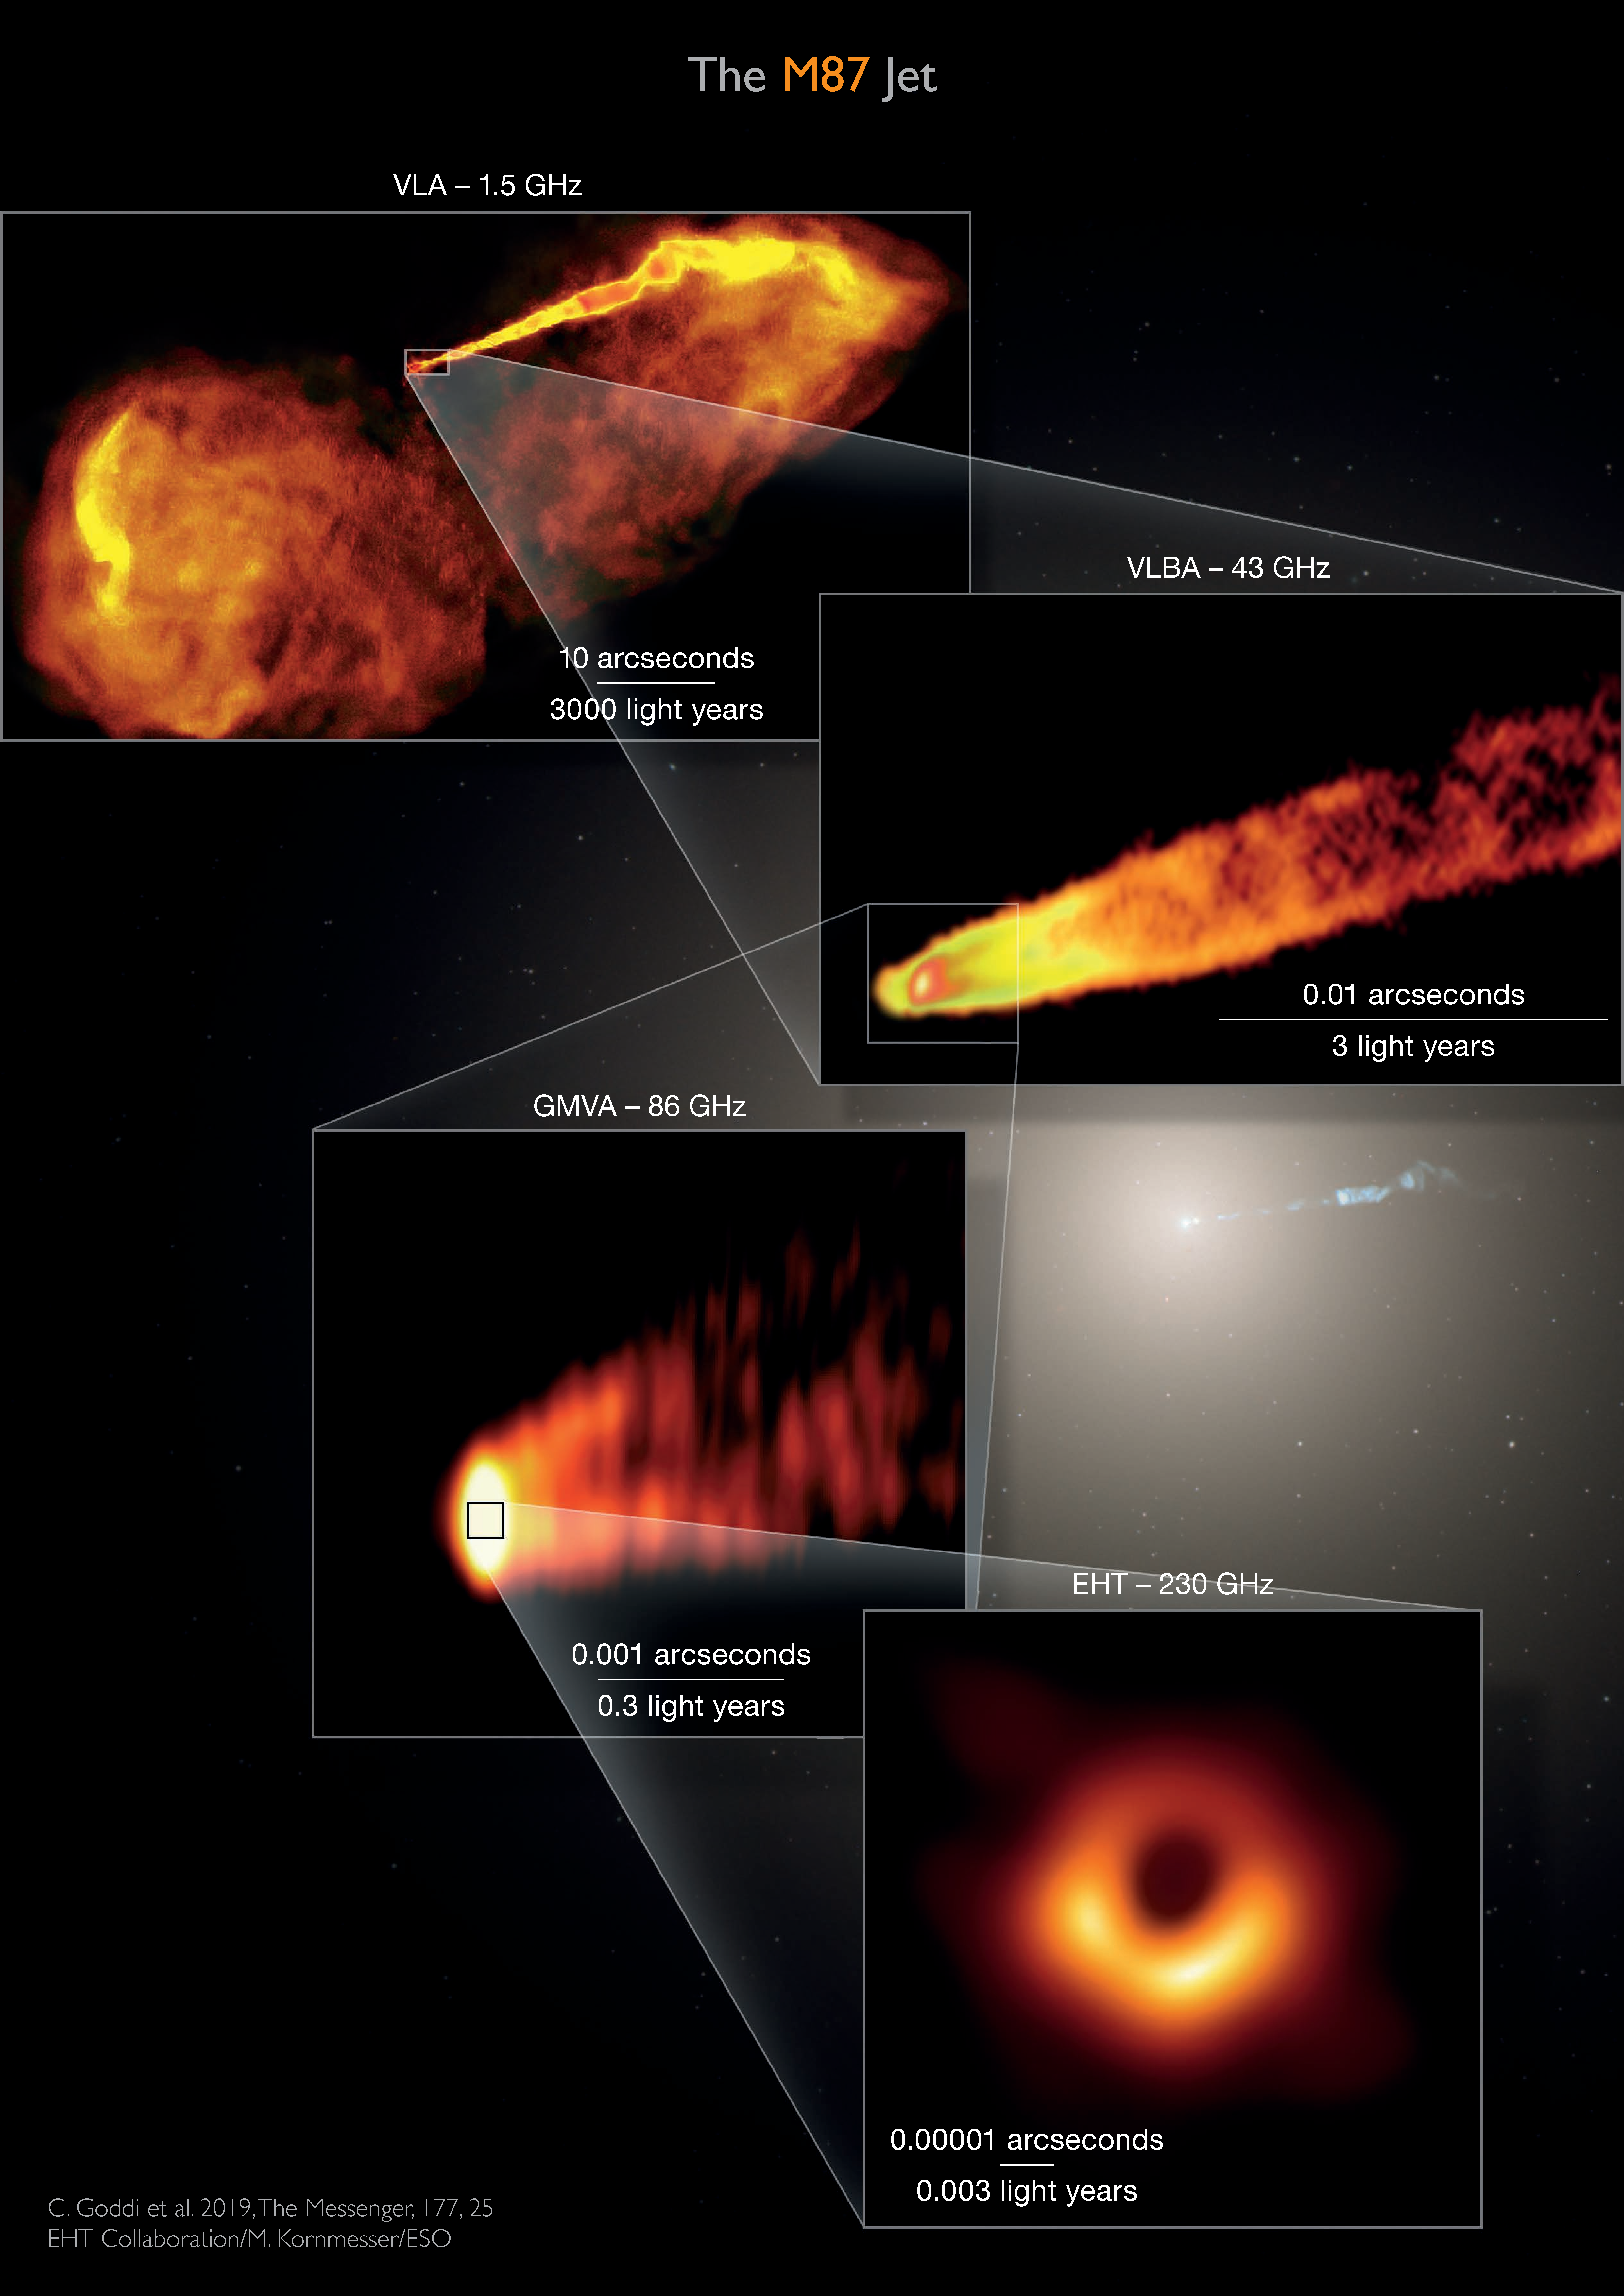
\includegraphics[width=0.96\linewidth,height=0.74\textheight,keepaspectratio]{../figs/pdf/en/fig-07-02.pdf}

% DOCX paragraph 892
\caption{\emph{Composición de imágenes de M87 a distintas radiofrecuencias y, por tanto, con distintas resoluciones angulares. © The EHT Collaboration/ESO/M. Kornmesser/C. Goddi/LR.}}\label{fig:07-02}
\end{figure}

% DOCX paragraph 894
En el fondo de la figura \ref{fig:07-02} aparece una imagen de toda la galaxia M87 tomada en la banda óptica. Se ve como un objeto de luminosidad difusa y núcleo brillante, del que emerge hacia la derecha un chorro semejante a un penacho de humo colimado. El chorro que se mueve hacia la izquierda queda absorbido casi por completo a estas longitudes de onda.

% DOCX paragraph 895
A estas alturas creo que está claro por qué una imagen como la del EHT es la primera de su clase. Para producirla e interpretarla hubo que reunir a muchos científicos de todas las etapas del proceso, desde la observación hasta la teoría. Como en otros proyectos de este tipo, el éxito depende inevitablemente de disponer de recursos económicos considerables para financiar el trabajo de tanta gente. La comunidad científica europea ha hecho una aportación importante, si no esencial, de la que no podemos evitar sentirnos orgullosos. Gracias a los fondos que el Consejo Europeo de Investigación, o ERC\index{ERC (Consejo Europeo de Investigación)}, concedió en 2013 a mis colegas Heino Falcke, de la Universidad de Nimega, en los Países Bajos, Michael Kramer, del Instituto Max Planck de Bonn, en Alemania, y a mí, el EHT, fundado oficialmente en 2009, pudo «despegar» en 2014 como una colaboración eficaz y realizar las investigaciones necesarias. Los catorce millones de euros obtenidos mediante nuestra subvención ERC Synergy Grant, BlackHoleCam\index{BlackHoleCam}\textsuperscript{\hyperlink{note:07-02}{2}}, la mayor concedida por el ERC a la astronomía, permitieron formar un equipo de investigadores europeos de primera línea y actuaron como catalizador para conseguir fondos adicionales para los colegas americanos y asiáticos. Solo así, tras alcanzar la «masa crítica» necesaria, pudimos convertir en realidad la idea de fotografiar un agujero negro supermasivo.

% DOCX paragraph 896
Terminaré esta sección con una reflexión sobre el papel de la suerte en las actividades humanas, incluidas las que los científicos intentamos sustraer, en lo posible, a la voluntad del destino. Como hemos dicho, el EHT ha logrado la mayor resolución angular\index{resolución angular} alcanzada en radioastronomía para un agujero negro supermasivo. Aun así, apenas bastó para obtener con confianza una imagen de M87*\index{M87*}, cuya proyección en el cielo ocupa unas decenas de microsegundos de arco. Pero eso solo lo sabemos ahora que tenemos una estimación de la masa de M87*. Antes de 2017, la masa de M87* era incierta y las estimaciones diferían en un factor de dos. Si la masa de M87* hubiera sido dos veces menor, como sostenía una de ellas, su imagen en el cielo también habría sido dos veces menor y la resolución del EHT, por revolucionaria que fuera, habría resultado insuficiente. Como entonces no lo sabíamos, las observaciones de 2017 fueron, en parte, una apuesta con fundamento. Pero la lección es la de siempre: «fortuna iuvat audaces», la fortuna favorece a los audaces. Y en la colaboración EHT fuimos tan audaces como afortunados...

% DOCX paragraph 899
\section{Todo es cuestión de trayectorias}\label{sec:07-trajectories}

% DOCX paragraph 901
Ahora que conocemos mejor la tecnología de las observaciones VLBI, podemos dirigir la atención a lo que les ocurre a los rayos de luz cerca de un agujero negro. Conocer las trayectorias que puede seguir la luz es fundamental para comprender por qué la imagen de M87*\index{M87*} debe ser necesariamente como la de la figura \ref{fig:07-01}.

% DOCX paragraph 902
Ya vimos en el capítulo 3 que nada puede moverse en línea recta en un espaciotiempo curvado, ni siquiera los rayos de luz, los fotones, que pueden dar lugar a fenómenos de lente gravitatoria\index{gravitatorio!efecto de lente}. Como el espaciotiempo alcanza su curvatura máxima cerca de los agujeros negros, cabe esperar que los fotones sigan allí trayectorias muy curvadas. ¡Y así es!\index{foton@fotón!órbitas}

% DOCX paragraph 903
Podemos verlo en la figura \ref{fig:07-03}, que muestra las trayectorias de algunos fotones cerca de un agujero negro de Schwarzschild\index{agujero negro!Schwarzschild}, es decir, sin rotación. Sé que esta imagen puede intimidar o incluso resultar confusa a primera vista, pero vamos a recorrerla juntos, con paciencia, e intentar comprender toda la información que contiene.

% DOCX paragraph 905
\begin{figure}[htbp]
\centering
sin rotación\par\medskip

% DOCX paragraph 906
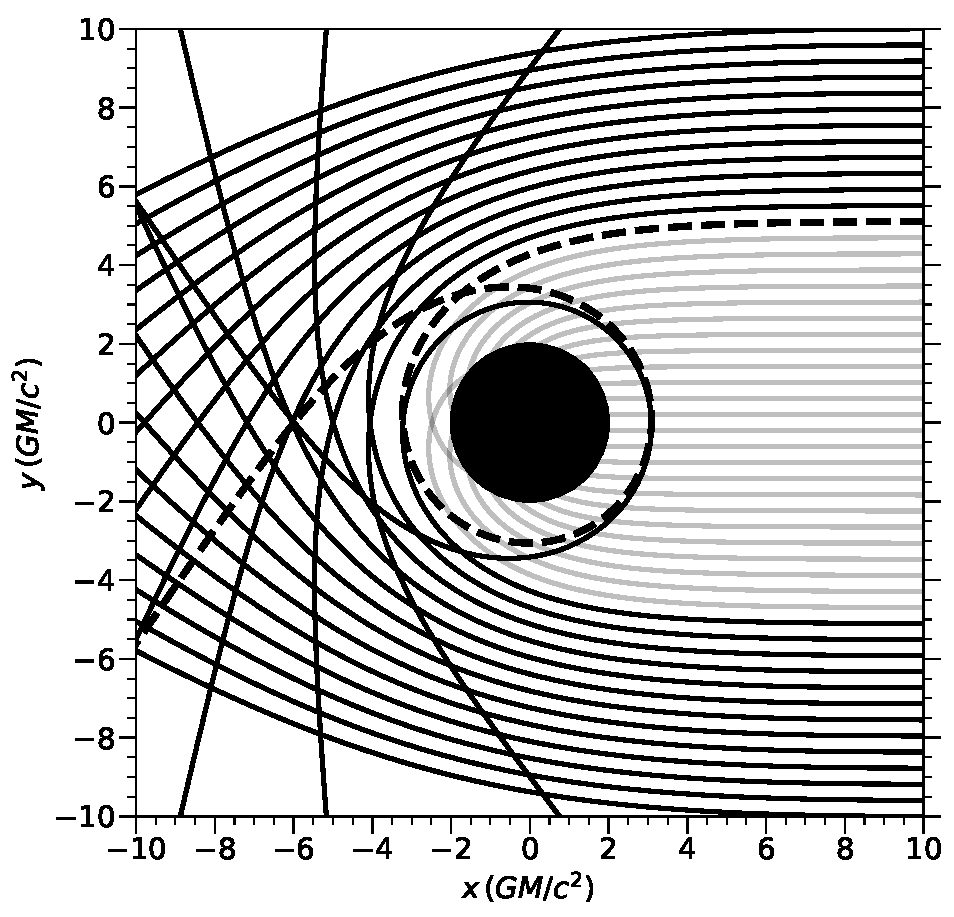
\includegraphics[width=0.88\linewidth,height=0.48\textheight,keepaspectratio]{../figs/pdf/en/fig-07-03.pdf}

% DOCX paragraph 908
\caption{\emph{Órbita\index{orbita@órbita!fotón}s de fotones en el plano ecuatorial de un agujero negro sin rotación, orientadas de derecha a izquierda. © C. Fromm/LR.}}\label{fig:07-03}
\end{figure}

% DOCX paragraph 910
Para empezar, la figura \ref{fig:07-03} representa el movimiento de los fotones en un plano ecuatorial. El círculo oscuro del centro es el horizonte de sucesos\index{horizonte de sucesos} del agujero negro visto desde arriba. Todas las trayectorias corresponden a rayos de luz emitidos desde la derecha de la figura, en \emph{x=10 (GM/c\textsuperscript{2})}. Puedes seguir cualquiera desde su origen; por ejemplo, la de más arriba comienza en \emph{x=10 (GM/c\textsuperscript{2})} e \emph{y=10 (GM/c\textsuperscript{2})}, y avanza de derecha a izquierda.\index{orbita@órbita!fotón}

% DOCX paragraph 911
Se ve que algunas trayectorias se desvían, pero no terminan en el agujero negro: son las líneas negras continuas. Otras, las líneas grises continuas, son capturadas y terminan dentro del horizonte de sucesos. Las trayectorias más alejadas del agujero negro se desvían poco, pero, a medida que se acercan o, más precisamente, disminuye el parámetro de impacto\textsuperscript{\hyperlink{note:07-03}{3}}, la desviación aumenta hasta superar los 90 grados. Entre las trayectorias capturadas, algunas entran «directamente» en el horizonte de sucesos sin desviarse mucho, mientras que otras son capturadas tras pasar cerca del agujero negro. Por último, una línea negra discontinua muestra un ejemplo de las extrañas trayectorias que pueden darse en sus proximidades. En este caso, el fotón parte de \emph{x=10 (GM/c\textsuperscript{2})} e \emph{y≃5,2 (GM/c\textsuperscript{2})}, se acerca al agujero negro, completa una vuelta a su alrededor y se aleja en \emph{x=-10 (GM/c\textsuperscript{2})} e \emph{y≃--5,5 (GM/c\textsuperscript{2})}. Es una órbita «extraña», como mínimo, pero pronto veremos que las hay aún más raras.

% DOCX paragraph 912
En la figura \ref{fig:07-03} podemos imaginar un límite entre las trayectorias negras, desviadas pero no capturadas, y las grises, desviadas y capturadas. Ese límite lo representa la órbita circular inestable\index{orbita@órbita!circular inestable (fotón)}\index{orbita@órbita!circular inestable (fotón)} de los fotones, o «\emph{anillo de luz\index{foton@fotón!anillo (de luz)}}», que para un agujero negro de Schwarzschild\index{agujero negro!Schwarzschild} se sitúa a un radio preciso\textsuperscript{\hyperlink{note:07-04}{4}}: \emph{r\textsubscript{po}=3 (GM/c\textsuperscript{2})}. Por tanto, la figura \ref{fig:07-03} nos muestra que debe existir una trayectoria muy especial para la luz alrededor de un agujero negro sin rotación. Si colocáramos con gran precisión un haz de luz en esa órbita, idealmente podría permanecer para siempre al mismo radio, en el anillo de fotones. Pero es una órbita «\emph{inestable}», y un fotón que la recorriera se sentiría como nosotros al caminar por la cresta afilada de una cordillera de laderas muy empinadas: la más leve perturbación nos haría caer hacia un lado. Del mismo modo, una perturbación mínima haría que el fotón abandonase el anillo de luz y cayera en el agujero negro o se alejara hacia el infinito.

% DOCX paragraph 913
Para ofrecer una imagen concreta de lo que les ocurre a los fotones cerca de un agujero negro, suelo utilizar una analogía con un arco y unas flechas. Imagina una diana de propiedades extraordinarias: como una diana corriente, puede recibir el impacto de una flecha que se cruce directamente con ella en su trayectoria. Pero, al ser especial, también puede recibirlo si la flecha pasa lo bastante cerca, pues la diana la obliga a girar a su alrededor, una o varias veces, hasta alcanzarla. Admito que a menudo he deseado que existiera una diana así: habría mejorado mucho mi puntería como arquero... Pues bien, eso es, en esencia, lo que les ocurre a los fotones que rozan el agujero negro por dentro del anillo de luz. No necesitan alcanzar directamente el horizonte de sucesos\index{horizonte de sucesos}, porque antes o después caerán en él. Pronto veremos cómo la trayectoria límite del anillo de luz desempeña un papel decisivo en las observaciones.

% DOCX paragraph 916
\section[El movimiento de vórtice]{El movimiento de vórtice cerca de un agujero negro en rotación}\label{sec:07-rotation}

% DOCX paragraph 918
El comportamiento de los rayos de luz de la figura \ref{fig:07-03} puede extenderse también a los agujeros negros en rotación, o de Kerr, que constituyen la gran mayoría de los agujeros negros del universo. Pero antes de estudiar la luz cerca de ellos, debemos presentar una característica importante de la que aún no hemos hablado. Hemos visto que los agujeros negros producen una curvatura extrema en el espaciotiempo que los rodea. Por la misma razón, si están girando, cabe esperar que su movimiento induzca también una «rotación» del espaciotiempo. Dicho de otro modo, es razonable pensar que un agujero negro en rotación genere una especie de vórtice de curvatura a su alrededor, obligando a los objetos cercanos a girar con él.

% DOCX paragraph 919
Para entender lo que ocurre, imaginemos una partícula de prueba\index{partícula de prueba} a gran distancia de un agujero negro en rotación. La partícula no tiene momento angular, es decir, no gira respecto a un sistema de referencia local. Si la dejamos caer, se dirigirá hacia el agujero negro siguiendo una trayectoria que, al menos al principio, será puramente radial. Pero al acercarse sucede algo extraño: para un observador lejano, la trayectoria deja de ser puramente radial y adquiere un movimiento en espiral, como si la partícula girara en el mismo sentido que el agujero negro. No sorprende que, si repitiéramos exactamente el mismo experimento con un agujero negro sin rotación, el resultado fuera muy distinto: la partícula seguiría una trayectoria radial hasta alcanzar el horizonte de sucesos. Esta rotación inducida de una partícula de prueba se conoce técnicamente como «arrastre de sistemas de referencia inerciales» y es una propiedad característica de los agujeros negros en rotación.

% DOCX paragraph 920
El arrastre del espaciotiempo circundante no es exclusivo de los agujeros negros: también ocurre en las estrellas de neutrones y los planetas, ¡y se ha medido incluso para la Tierra! Sin embargo, una vez más, el fenómeno alcanza una intensidad extrema en los agujeros negros. Un agujero negro en rotación tiene una superficie muy especial situada fuera del horizonte de sucesos\index{horizonte de sucesos}, llamada «\emph{ergosfera\index{agujero negro!ergosfera}\index{ergosfera|see{agujero negro}}}» o «\emph{límite estático\index{límite estático}}». Sus propiedades permiten que cualquier objeto, con masa o sin ella, gire en sentido contrario al agujero negro, es decir, contrarrote, mientras se encuentre fuera de la ergosfera. Pero, una vez que la cruza, ya no puede resistirse a la rotación del agujero negro y se ve obligado a girar en el mismo sentido, es decir, a corrotar.\index{orbita@órbita!en contrarrotación}

% DOCX paragraph 921
Para comprender mejor la ergosfera, podemos volver a la analogía del capítulo anterior: un agujero negro sin rotación y un lago con un agujero en el fondo. Imaginábamos una cascada circular en la que el agua caía siguiendo trayectorias radiales. Ahora supongamos que el agujero gira o, de forma equivalente, que el agua tiene cierto momento angular. Esto crearía un vórtice cerca de la cascada: lejos del agujero, la corriente sería esencialmente radial, pero al acercarse se volvería cada vez más circular. Si estuviéramos en una embarcación y dejáramos que la corriente nos llevara, giraríamos con el resto del agua. A una distancia suficientemente grande, podríamos usar los potentes motores para resistir la corriente y girar en sentido contrario al agujero, aunque esto sería cada vez más difícil al acercarnos a la cascada. Habría un punto crítico más allá del cual, por potentes que fueran los motores, no podríamos girar contra la corriente y nos veríamos obligados a corrotar. Ese punto crítico es el equivalente mecánico de la ergosfera de un agujero negro en rotación.

% DOCX paragraph 922
Es esencial subrayar que, dentro de la ergosfera\index{agujero negro!ergosfera}, ya no podemos oponernos al sentido de rotación impuesto por el agujero negro, pero seguimos fuera del horizonte de sucesos. Por tanto, en principio aún podemos salir, por ejemplo mediante un movimiento parcialmente radial que nos lleve a gran distancia del agujero negro. Esto es posible porque el borde exterior de la ergosfera no se comporta como un horizonte de sucesos: está a un radio mayor que este y permite el movimiento tanto hacia dentro como hacia fuera.

% DOCX paragraph 923
La figura \ref{fig:07-04} lo ilustra de forma muy esquemática: muestra el movimiento de vórtice del espaciotiempo cerca de un agujero negro y el borde exterior de la ergosfera, situado claramente a un radio mayor que el horizonte de sucesos\index{horizonte de sucesos}. Fuera de la ergosfera es posible contrarrotar. Entre ella y el horizonte de sucesos, en cambio, no podemos contrarrotar, aunque sí alejarnos a grandes distancias. Dentro del horizonte de sucesos, el único movimiento posible es radial y hacia dentro, cayendo hacia la singularidad física\index{singularidad!física}.

% DOCX paragraph 925
\begin{figure}[htbp]
\centering
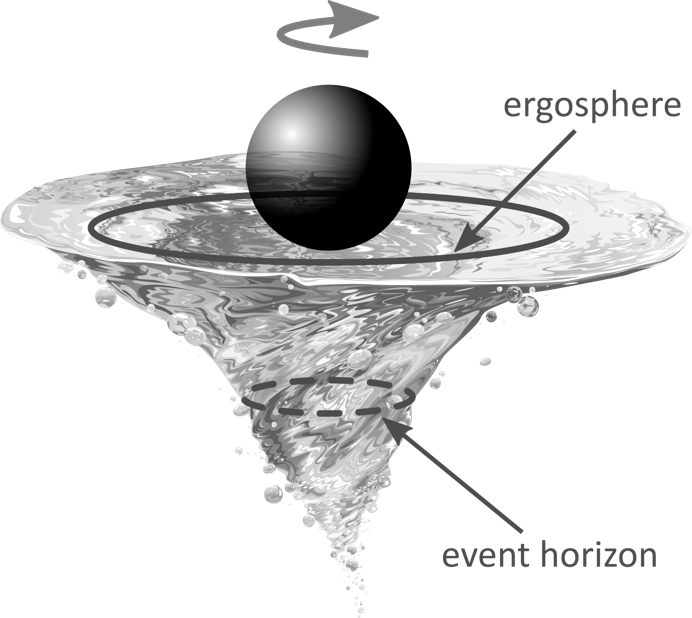
\includegraphics[width=0.88\linewidth,height=0.48\textheight,keepaspectratio]{../figs/source/en/fig-07-04.png}

% DOCX paragraph 927
\caption{\emph{Movimiento de vórtice de la materia cerca de un agujero negro y posición del borde exterior de la ergosfera\index{agujero negro!ergosfera}, situado claramente a un radio mayor que el horizonte de sucesos. © Jullands/depositphotos.com/LR.}}\label{fig:07-04}
\end{figure}

% DOCX paragraph 929
Veamos algunos números: para un agujero negro de Kerr\index{agujero negro!Kerr} que gira casi a la máxima velocidad permitida, es decir, con espín adimensional \emph{a ≃ 1}, el horizonte de sucesos está a un radio \emph{r\textsubscript{+}≃GM/c\textsuperscript{2}}, mientras que el borde exterior de la ergosfera está a un radio casi dos veces mayor, \emph{r\textsubscript{0}≃2 (GM/c\textsuperscript{2})}.

% DOCX paragraph 930
Además de la corrotación forzada, la ergosfera es una región en la que pueden darse proceso\index{Penrose!proceso}s físicos fascinantes. Las partículas pueden acelerarse hasta velocidades muy altas y la energía\index{energia@energía!de rotación} rotacional del agujero negro, es decir, su masa reducible, puede extraerse mediante el «proceso de Penrose», llamado así por el físico británico Roger\index{Penrose!Roger} Penrose, que lo describió por primera vez en los años setenta\textsuperscript{\hyperlink{note:07-05}{5}}. Mucho podríamos decir sobre este asunto, pero nos alejaría demasiado de nuestro objetivo...

% DOCX paragraph 931
Volvamos a los rayos de luz y examinemos sus trayectorias cerca de un agujero negro en rotación. La figura \ref{fig:07-05} muestra tanto el caso de un agujero negro que gira en el sentido de las agujas del reloj, en el recuadro izquierdo, como el de otro que gira en sentido contrario, en el derecho. En ambos casos los observamos desde arriba, a lo largo del eje de rotación.

% DOCX paragraph 938
\begin{figure}[htbp]
\centering
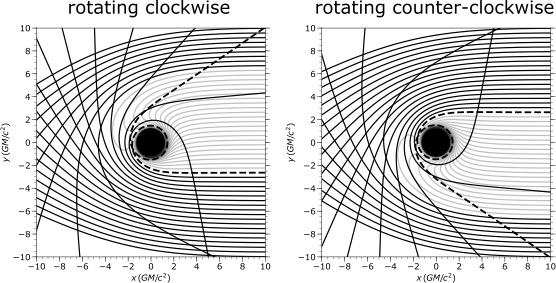
\includegraphics[width=0.88\linewidth,height=0.48\textheight,keepaspectratio]{../figs/source/en/fig-07-05.jpeg}

% DOCX paragraph 940
\caption{\emph{Las mismas órbitas de la figura \ref{fig:07-03}, pero para agujeros negros en rotación. La rotación crea una vorticidad en las trayectorias, y los fotones deben adaptarse a su sentido de giro. Al mismo tiempo, el horizonte de sucesos es significativamente menor. © C. Fromm/LR.}}\label{fig:07-05}
\end{figure}

% DOCX paragraph 942
Creo que está claro que la rotación del agujero negro rompe la simetría esférica\index{simetría esférica} de la figura \ref{fig:07-03}, de modo que la posibilidad de capturar un fotón\index{foton@fotón!órbita} depende del lado por el que este se aproxime. Si se acerca por el lado que gira en su mismo sentido, por ejemplo desde valores negativos de la coordenada \emph{y} en el caso del agujero negro que gira como las agujas del reloj, le resultará más fácil llegar muy cerca del horizonte de sucesos\index{horizonte de sucesos} sin ser capturado. En la figura \ref{fig:07-05}, podemos apreciarlo al comparar la transición entre las líneas negras y grises alrededor de \emph{y=0}, o simplemente comparando las figuras 7.3 y 7.5.

% DOCX paragraph 943
Además, si miras con atención los dos recuadros de la figura \ref{fig:07-05}, podrás reconocer la ergosfera\index{agujero negro!ergosfera}. Basta fijarse en las órbita\index{orbita@órbita}\index{orbita@órbita!en corrotación}\index{foton@fotón!órbita}s de los fotones que se acercan en sentido contrario al giro, por ejemplo desde valores positivos de la coordenada \emph{y} en el agujero negro que gira como las agujas del reloj. En cierto punto, los fotones se ven obligados a cambiar de dirección y corrotar con el agujero negro. Como la única diferencia entre los dos recuadros es el sentido de rotación, las imágenes son equivalentes y antisimétricas: podemos obtener una a partir de la otra mediante una simple rotación alrededor del eje \emph{x}.\index{foton@fotón!en corrotación}\index{foton@fotón!en contrarrotación}

% DOCX paragraph 944
Ten en cuenta que solo hemos visto una pequeña parte del panorama: nos hemos limitado a órbitas de fotones situadas en un mismo plano, concretamente el plano ecuatorial del agujero negro. La dinámica de la luz es mucho más compleja para órbitas arbitrarias, que no estén obligadas a moverse en un plano determinado. Este caso es la regla, pues solo una pequeña fracción de las órbitas posibles está contenida en un plano, y en él los rayos de luz se comportan de forma mucho más extraña.

% DOCX paragraph 945
La figura \ref{fig:07-06} muestra un ejemplo de órbita genérica\index{orbita@órbita!genérica}, elegido al azar entre millones que podría producir. Representa la trayectoria de un fotón alrededor de un agujero negro que gira en el sentido de las agujas del reloj. El recuadro izquierdo ofrece una reconstrucción tridimensional de la órbita; el derecho muestra sus proyecciones en dos planos y ayuda a comprender su dinámica. Fíjate en que la órbita es mucho más compleja, aunque te aseguro que las hay aún peores, y en que el fotón puede acercarse mucho al agujero negro y dar al menos cuatro vueltas sin ser capturado. Al final se desvía en una dirección casi diametralmente opuesta a la inicial. Además, como el fotón no es absorbido, la órbita es simétrica bajo «inversión temporal\index{inversión temporal}»: da igual por qué extremo empecemos a seguirla, pues puede recorrerse en ambos sentidos.

% DOCX paragraph 946
\begin{figure}[htbp]
\centering
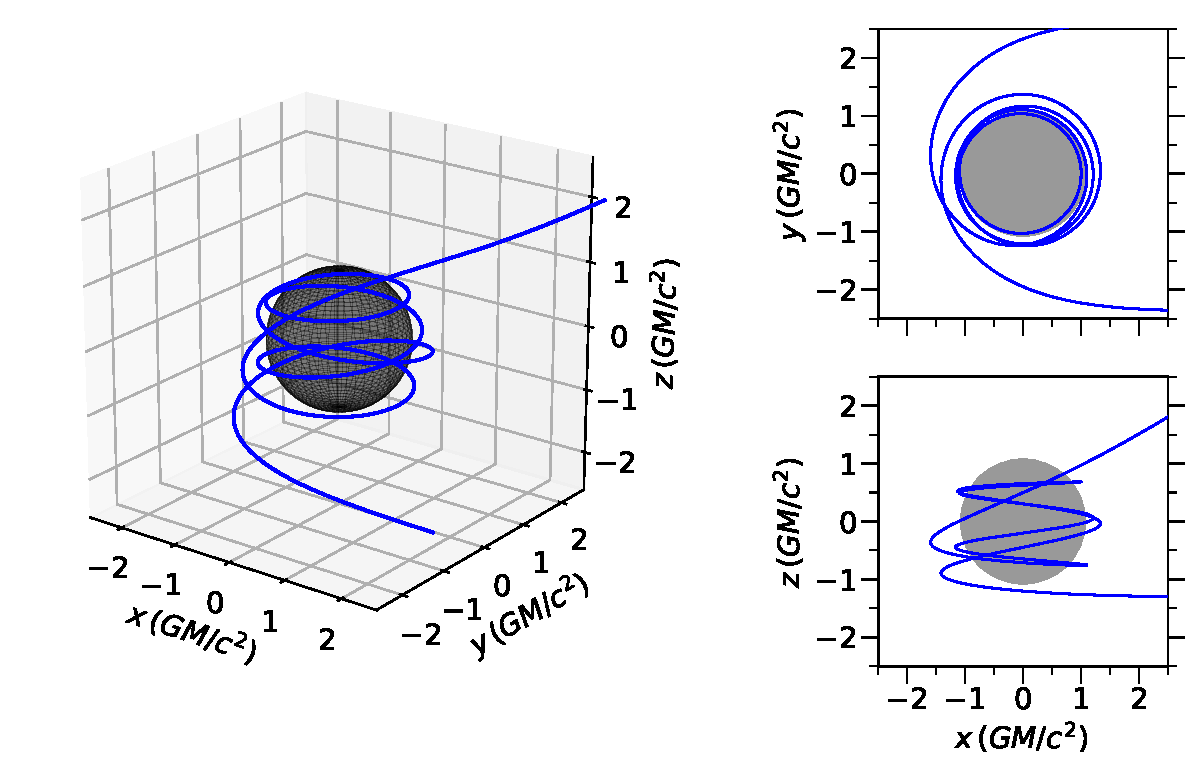
\includegraphics[width=0.88\linewidth,height=0.48\textheight,keepaspectratio]{../figs/pdf/en/fig-07-06.pdf}

% DOCX paragraph 948
\caption{\emph{Órbita genérica de un fotón alrededor de un agujero negro en rotación. © C. Fromm/LR.}}\label{fig:07-06}
\end{figure}

% DOCX paragraph 950
Como hemos dicho, la complejidad de la trayectoria de la figura \ref{fig:07-06} es la regla, no la excepción. Basta modificar un poco las condiciones iniciales para obtener incontables variantes igual de complejas y curiosas. Esta propiedad tiene implicaciones importantes para lo que veremos cuando explique cómo se «produjo» la imagen de M87*\index{M87*} del EHT a partir de las observaciones. Si la dinámica de la luz cerca de un agujero negro puede ser tan compleja y un fotón puede regresar por donde vino, algo muy ajeno a nuestra experiencia del espaciotiempo plano, reconstruir una imagen a partir de todas esas órbitas será muy complicado. Supongamos que la luz puede emitirse y recibirse desde cualquier dirección. Podríamos temer incluso que fuera imposible obtener una foto coherente de las regiones cercanas al agujero negro, o que las imágenes fueran manchas amorfas de intensidad sin ningún detalle. Pero la radiación no se emite en todas partes, sino en regiones concretas, y una parte es absorbida por el agujero negro y no nos alcanza. Esto da lugar a un atractivo juego de luces y sombras que, en condiciones astrofísicas realistas, se combinan en una imagen de propiedades muy particulares, como veremos.

% DOCX paragraph 953
\section{Un juego de luces y sombras}\label{sec:07-shadow}

% DOCX paragraph 955
Acabamos de ver lo compleja que puede ser la trayectoria de la luz en un espaciotiempo curvado, sobre todo cerca de un agujero negro. Incluso hemos aprendido que un fotón puede regresar al lugar donde fue emitido. Son comportamientos muy distintos de los que conocemos en la Tierra, donde la luz viaja esencialmente en línea recta y vemos lo que tenemos delante, no lo que queda detrás de nosotros. Si tenemos un objeto enfrente, recibimos su imagen directa y no una imagen indirecta de lo que hay detrás de él. Piensa lo sorprendente que sería acercarte a un hombre con traje y corbata y ver también la mancha que lleva en la espalda. ¡Pues todo esto es posible cerca de un agujero negro!

% DOCX paragraph 956
Para complicar aún más las cosas, la luz no solo cambia de dirección: también puede «desaparecer» al ser capturada por el agujero negro. Está claro que, para entender lo que ocurre y saber qué esperar, debemos reeducar nuestra percepción\index{percepción} de lo posible y lo imposible en condiciones de curvatura extrema. Consideraremos formas geométricas precisas que correspondan a posibles fuentes de luz alrededor de un agujero negro y deduciremos cómo las vería un observador a distancia astronómica. Descubriremos que una parte considerable de los rayos puede desaparecer y crear regiones oscuras, o «sombras», pero también que pueden concentrarse y amplificarse como a través de una lente.

% DOCX paragraph 957
La figura \ref{fig:07-07} muestra el caso más sencillo, que permite apreciar algunas de las sutilezas de producir la imagen de un objeto cerca de un agujero negro. Representa un agujero negro sin rotación y aislado, sin materia a su alrededor, cuyo horizonte de sucesos\index{horizonte de sucesos} aparece como una pequeña esfera gris. El agujero negro está delante de una fuente luminosa, por ejemplo un hermoso cielo estrellado, representada esquemáticamente a la izquierda. Queremos comprender qué le ocurre a un haz de luz emitido por esa fuente y cómo lo recibe un observador lejano situado a la derecha.

% DOCX paragraph 959
\begin{figure}[htbp]
\centering
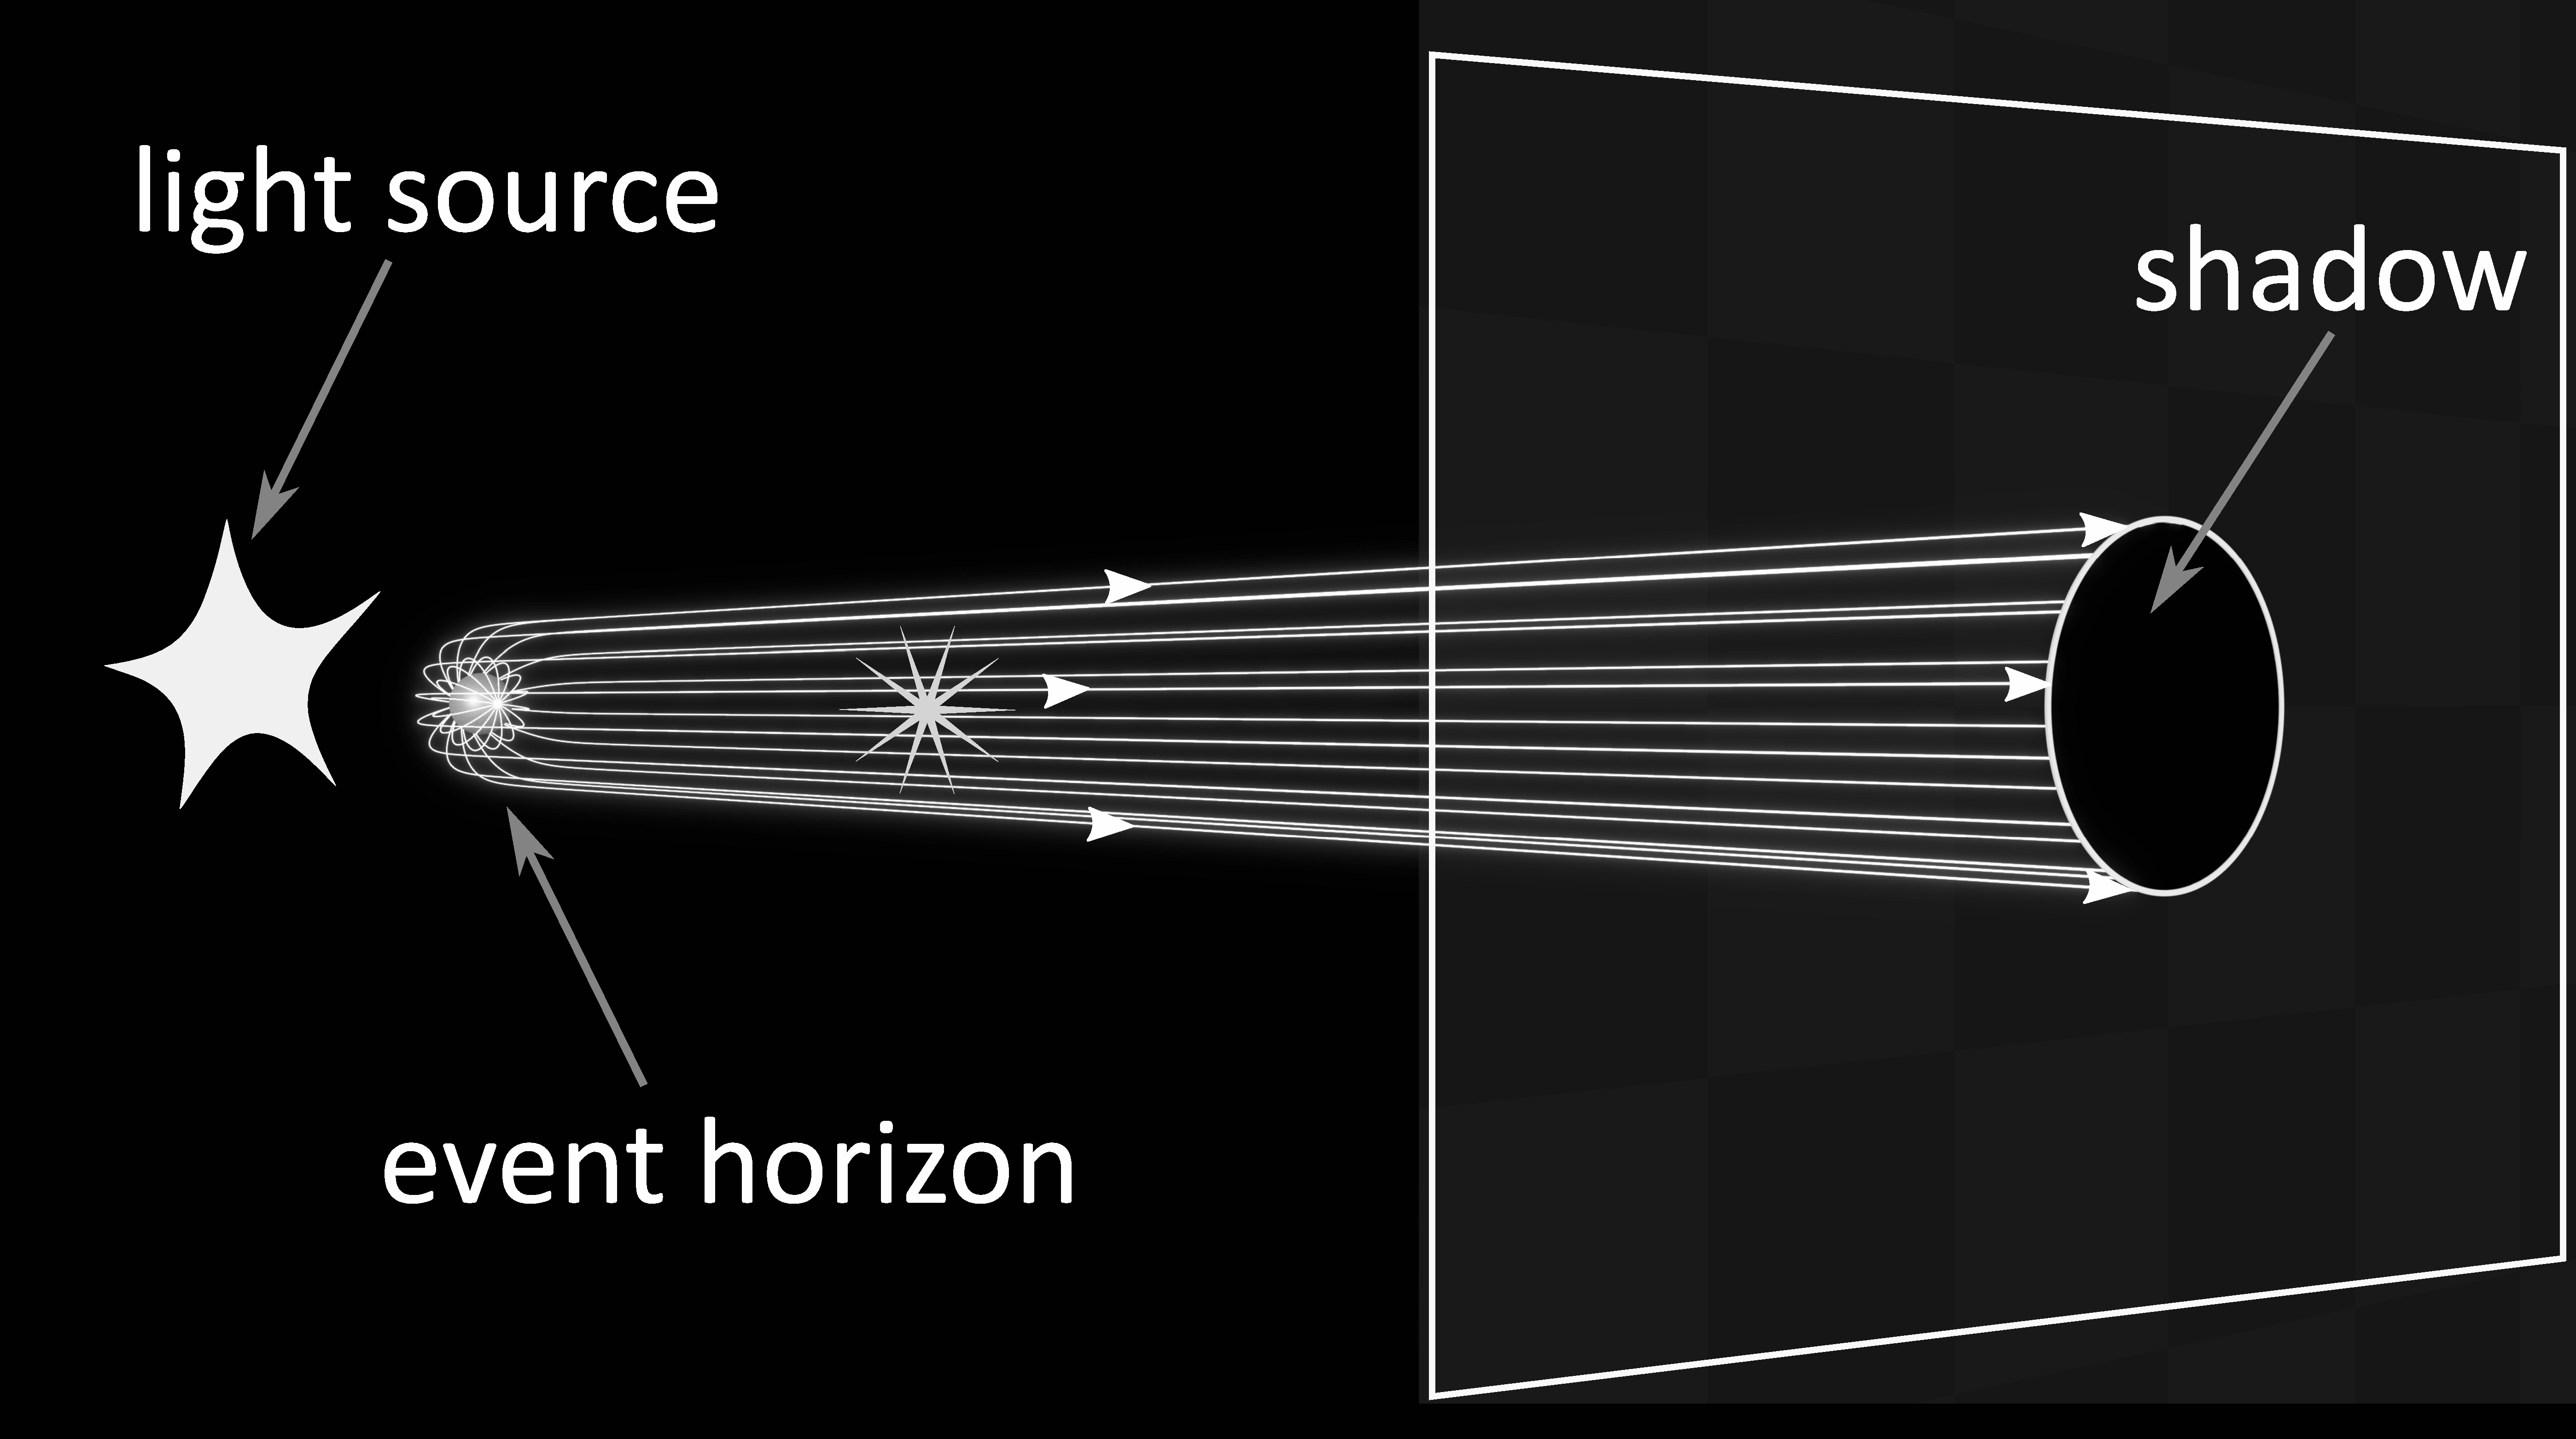
\includegraphics[width=0.88\linewidth,height=0.48\textheight,keepaspectratio]{../figs/pdf/en/fig-07-07.pdf}

% DOCX paragraph 961
\caption{\emph{Creación de la «sombra\index{sombra (agujero negro)}» de un agujero negro. © T. Müller/M. Pössel (MPIA)/LR.}}\label{fig:07-07}
\end{figure}

% DOCX paragraph 963
A estas alturas deberías tener una idea bastante clara de lo que le ocurre a un haz de luz dirigido hacia un agujero negro y poder imaginar lo que vería en su cielo un observador lejano. El agujero negro absorberá de inmediato una parte de los fotones emitidos, aquellos cuyas trayectorias corten la superficie esférica del horizonte de sucesos. Otros no la atravesarán directamente, pero pasarán lo bastante cerca como para desviarse y ser capturados. El límite de las trayectorias que «escaparán» a la captura viene dado por la órbita circular inestable de los fotones, o anillo de luz. Así, un observador lejano verá una región casi sin luz, porque el agujero negro habrá interceptado los fotones que deberían haberle llegado. Lo que verá será, por tanto, la «sombra\index{foton@fotón!sombra}\index{sombra (agujero negro)}» del agujero negro.

% DOCX paragraph 964
Este fenómeno tan básico como fundamental nos lleva a tres consideraciones útiles para eliminar algunas leyendas urbanas o ideas equivocadas sobre las sombra\index{sombra (agujero negro)}s de los agujeros negros. La primera es que observar la sombra no significa observar el horizonte de sucesos\index{horizonte de sucesos}. La sombra no depende solo de los fotones que inciden directamente en el horizonte, sino también de los que se acercan a una distancia menor que el anillo de luz. Además, al ser una imagen proyectada en el cielo, es necesariamente mayor incluso que el propio anillo. Más precisamente, el borde de la sombra, y por tanto su tamaño, se define mediante el parámetro de impacto de la órbita circular inestable\index{orbita@órbita!circular inestable (fotón)}\index{foton@fotón!órbita circular inestable} de los fotones. Para un agujero negro sin rotación, su radio es \emph{r\textsubscript{sh}=}\(\sqrt{27}\)\emph{(GM/c\textsuperscript{2})}. Como \(\sqrt{27} \simeq 5{,}2\), la sombra, la zona más oscura del centro de la figura \ref{fig:07-01}, es casi tres veces mayor que el horizonte de sucesos, \emph{r\textsubscript{S}=2(GM/c\textsuperscript{2})}. Además, el tamaño de la sombra, como el del horizonte, es proporcional a la masa del agujero negro: cuanto más masivo sea, mayor será su imagen en el cielo y más fácil resultará fotografiarlo a una distancia dada.

% DOCX paragraph 965
La segunda consideración es que la sombra representa una región del cielo en la que «falta luz», la que ha absorbido el agujero negro. Pero esa región no tiene por qué carecer por completo de luz. Solo el horizonte de sucesos no puede emitirla, de modo que es perfectamente normal que la zona de la sombra contenga algo de radiación. Un fotón emitido por una fuente situada entre el horizonte y un observador lejano, como la pequeña estrella blanca de la figura \ref{fig:07-07}, no sería absorbido si se dirigiera hacia el observador. Por eso, la sombra de M87*\index{M87*} en la figura \ref{fig:07-01} no es completamente oscura. De hecho, el EHT ha utilizado el contraste de intensidad entre el centro de la imagen y el anillo luminoso para acotar las propiedades de M87*.

% DOCX paragraph 966
La tercera y última consideración es que, salvo para un agujero negro sin rotación, cuya simetría esférica\index{simetría esférica} garantiza una sombra\index{sombra (agujero negro)} siempre igual, un círculo perfecto, la forma de la sombra depende tanto del espín del agujero negro como de la inclinación de la observación respecto al eje de rotación. Como adelantamos, la rotación del agujero negro hace girar todo el espaciotiempo cercano, mediante el efecto de arrastre de sistemas de referencia. Así, los fotones que se aproximan por un lado pueden llegar más cerca del horizonte de sucesos que los que se acercan por el lado opuesto (véase la figura \ref{fig:07-05}).

% DOCX paragraph 967
La rotación y la consiguiente pérdida de simetría esférica\index{simetría esférica} tienen otra consecuencia: la sombra cambia de aspecto según el ángulo de observación. La sombra de un agujero negro en rotación parecerá perfectamente circular si la observamos en la dirección polar, desde el Polo Norte o el Polo Sur. En cambio, desde el plano ecuatorial aparecerá deformada.

% DOCX paragraph 973
\section{Sombras y discos}\label{sec:07-discs}

% DOCX paragraph 975
Como la forma de la sombra\index{sombra (agujero negro)} depende del espín del agujero negro, en principio es posible deducirlo «simplemente» midiendo esa forma. En realidad, todo es bastante más complicado que en esta descripción, y medir con precisión la forma de la sombra sigue siendo muy difícil con las observaciones actuales. Esa es, en esencia, la razón por la que el EHT no ha podido medir el espín de M87*\index{M87*}, aunque es improbable que se trate de un agujero negro de Schwarzschild\index{agujero negro!Schwarzschild}. Volveremos sobre ello al comparar las observaciones con las predicciones teóricas.

% DOCX paragraph 976
Dejando de lado las enormes dificultades técnicas que aún debemos superar para obtener una imagen nítida de la sombra, su forma sigue siendo una herramienta formidable para comprender las propiedades del agujero negro. Toda la información sobre su masa, espín y carga, sus únicas tres propiedades, está impresa, aunque sea sutilmente, en su sombra. Me resulta tan fascinante como paradójico que podamos arrojar luz sobre los agujeros negros midiendo cómo señalan la ausencia de luz. Esto es cierto en general: se aplica tanto a los agujeros negros de la relatividad general como a los de teorías alternativas e incluso a objetos compactos que no son agujeros negros. Retomaremos estas ideas cuando nos preguntemos si M87*\index{M87*} es realmente un agujero negro...

% DOCX paragraph 977
Nos espera ahora un salto cualitativo importante para comprender qué rasgos debería tener una imagen realista de M87*\index{M87*}. Hasta aquí hemos considerado las condiciones muy idealizadas de un agujero negro aislado ante un fondo de fuentes luminosas. En condiciones astrofísicas realistas, sin embargo, lo rodea un plasma a temperaturas y energías elevadas, que cae sobre él en forma de disco de acreción. ¿Qué aspecto tiene un agujero negro en esas condiciones?

% DOCX paragraph 978
La respuesta breve es que tendrá un aspecto muy distinto del que esperaríamos en un espaciotiempo plano. Para la respuesta larga, debemos recurrir de nuevo a una idealización. En lugar de considerar la imagen de un disco de acreción realista, cuyas propiedades resultan de sofisticadas simulaciones numéricas, empezaremos por modelizarlo con una forma geométrica más sencilla. Esto nos ayudará a comprender algunas de las propiedades más llamativas de los efectos de lente gravitatoria, las distorsiones de una imagen debidas a la curvatura del espaciotiempo, que caracterizan la imagen de un disco de acreción alrededor de un agujero negro.

% DOCX paragraph 979
Consideremos un disco de acreción\index{disco de acreción!delgado} formado por un anillo de materia de pequeño espesor vertical, centrado en el agujero negro. Dicho de otro modo, imaginemos que colocamos una rosquilla muy fina alrededor del agujero negro y nos preguntamos qué aspecto tendría vista desde muy lejos y con cierto ángulo.

% DOCX paragraph 980
Eso es precisamente lo que muestra la figura \ref{fig:07-08}: a la izquierda, un agujero negro rodeado por un disco fino de materia; a la derecha, la imagen que recibe un observador situado con cierto ángulo de inclinación. Hay una diferencia importante respecto a la figura \ref{fig:07-07}: ahora el agujero negro no está iluminado por una fuente extensa detrás de él. El propio disco de acreción\index{disco de acreción!delgado} actúa como fuente luminosa y, por tanto, puede aparecer deformado por la distorsión de las trayectorias de la luz alrededor del agujero negro.

% DOCX paragraph 981
\begin{figure}[htbp]
\centering
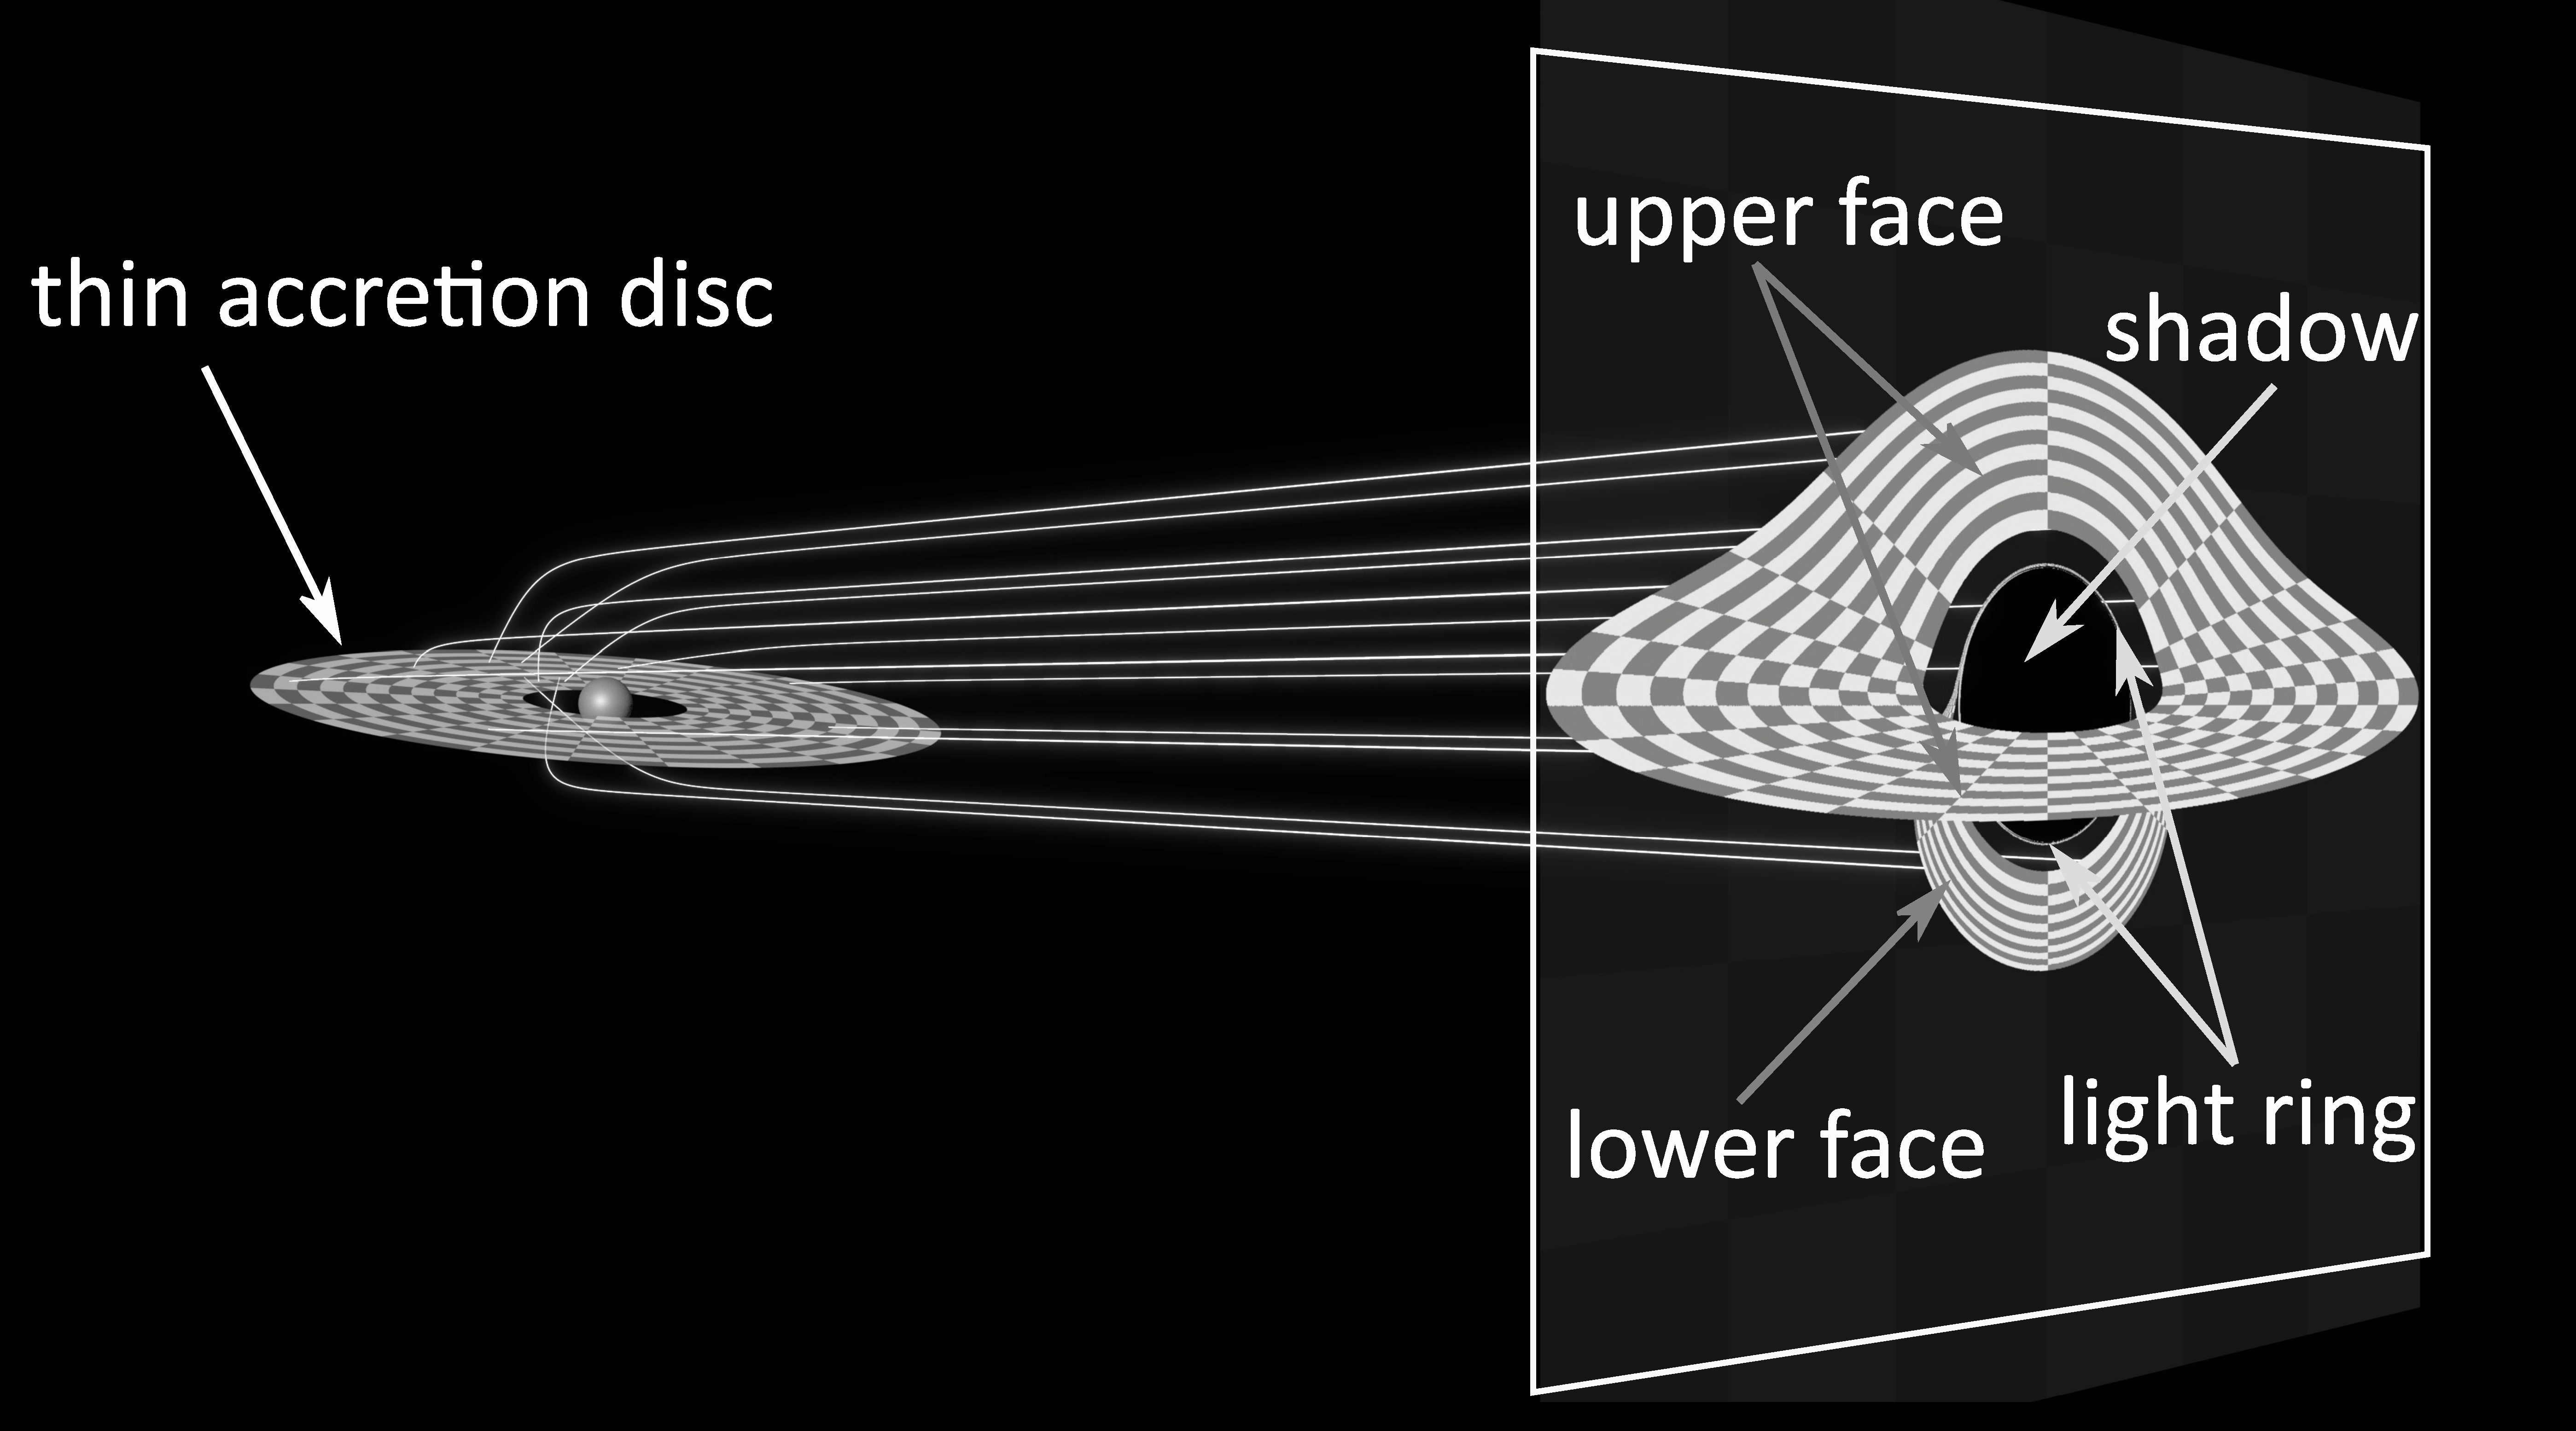
\includegraphics[width=0.88\linewidth,height=0.48\textheight,keepaspectratio]{../figs/pdf/en/fig-07-08.pdf}

% DOCX paragraph 983
\caption{\emph{Aspecto de un disco de acreción muy fino para un observador lejano. © T. Müller/M. Pössel (MPIA)/LR.}}\label{fig:07-08}
\end{figure}

% DOCX paragraph 985
En un espaciotiempo plano\index{espaciotiempo!plano} veríamos solo la parte del disco más cercana a nosotros, la parte delantera de su cara superior, pues desde ahí los fotones que viajan en línea recta pueden alcanzar nuestros ojos. Pero el disco está en una región de espaciotiempo muy curvado, ¡y la imagen es muy distinta! La figura \ref{fig:07-08} muestra que la «rosquilla» está muy distorsionada. No solo vemos la parte delantera de la cara superior, sino también su parte trasera, situada detrás del agujero negro y que no podríamos ver en un espaciotiempo plano. Es un efecto extraño, desde luego, pero perfectamente normal en un espaciotiempo curvado. Además, nos enseña una lección importante: si te encuentras en el espacio y necesitas esconderte, ¡no te pongas detrás de un agujero negro! No serviría de nada y solo revelaría lo poco que sabes de relatividad general...\index{foton@fotón}

% DOCX paragraph 986
Las rarezas no acaban ahí. La curvatura del espaciotiempo también nos permitiría ver la cara inferior de la parte trasera del disco, que aparecería abajo en la imagen como un apéndice colgante. En esencia, veríamos casi todo el disco. Conviene señalar que la sombra\index{sombra (agujero negro)} no sería una única región oscura, sino que quedaría dividida en dos: una visible por encima de la cara superior del disco y otra por debajo. Por último, también podríamos observar el anillo de luz, representado en la figura \ref{fig:07-08} como un anillo muy fino. A pesar de su finura, parecería relativamente luminoso, pues el espaciotiempo puede concentrar en él muchos fotones.

% DOCX paragraph 987
Si te gustan las películas de ciencia ficción tanto como a mí, sobre todo las que contienen una buena dosis de realismo y coherencia física, quizá hayas reconocido el disco de acreción de la derecha de la figura \ref{fig:07-08}. Se parece mucho al agujero negro supermasivo \emph{Gargantua}, protagonista de \emph{Interstellar} (2014), la película de Chris Nolan\index{Nolan, Chris (Interstellar)}. No es casualidad: la representación de Gargantua es bastante realista, aunque contiene al menos dos aspectos que no lo son.

% DOCX paragraph 988
El primero es que su disco de acreción se muestra geométricamente delgado, con una altura vertical muy pequeña. En realidad, las condiciones físicas del plasma en acreción\index{plasma!en acreción} cerca de un agujero negro supermasivo dan lugar a temperaturas y presiones muy altas dentro del disco, que lo obligan a «hincharse», sobre todo en las regiones más próximas al agujero negro. Por tanto, un disco realista es geométricamente grueso\index{disco de acreción!grueso}\index{disco de acreción!grueso}, con una altura vertical nada despreciable, como muestran las imágenes de la figura \ref{fig:07-09}. Los cuatro recuadros presentan cuatro ejemplos de un disco realista que emite radiación a una frecuencia de 230 GHz, calculados mediante una sofisticada simulación numérica. En cada imagen cambia el ángulo de inclinación del observador lejano, como indica el símbolo de la esquina inferior derecha, que también señala el sentido de rotación del plasma.

% DOCX paragraph 989
Fijémonos en los recuadros superior izquierdo e inferior derecho de la figura \ref{fig:07-09}. Ambos representan situaciones bastante generales y muestran que un disco de acreción realista tendría un aspecto más «esponjoso». Pero siguen siendo válidas las características básicas de la figura \ref{fig:07-08}: podemos ver las dos caras del disco y la sombra\index{sombra (agujero negro)} aparece duplicada.

% DOCX paragraph 990
\begin{figure}[htbp]
\centering
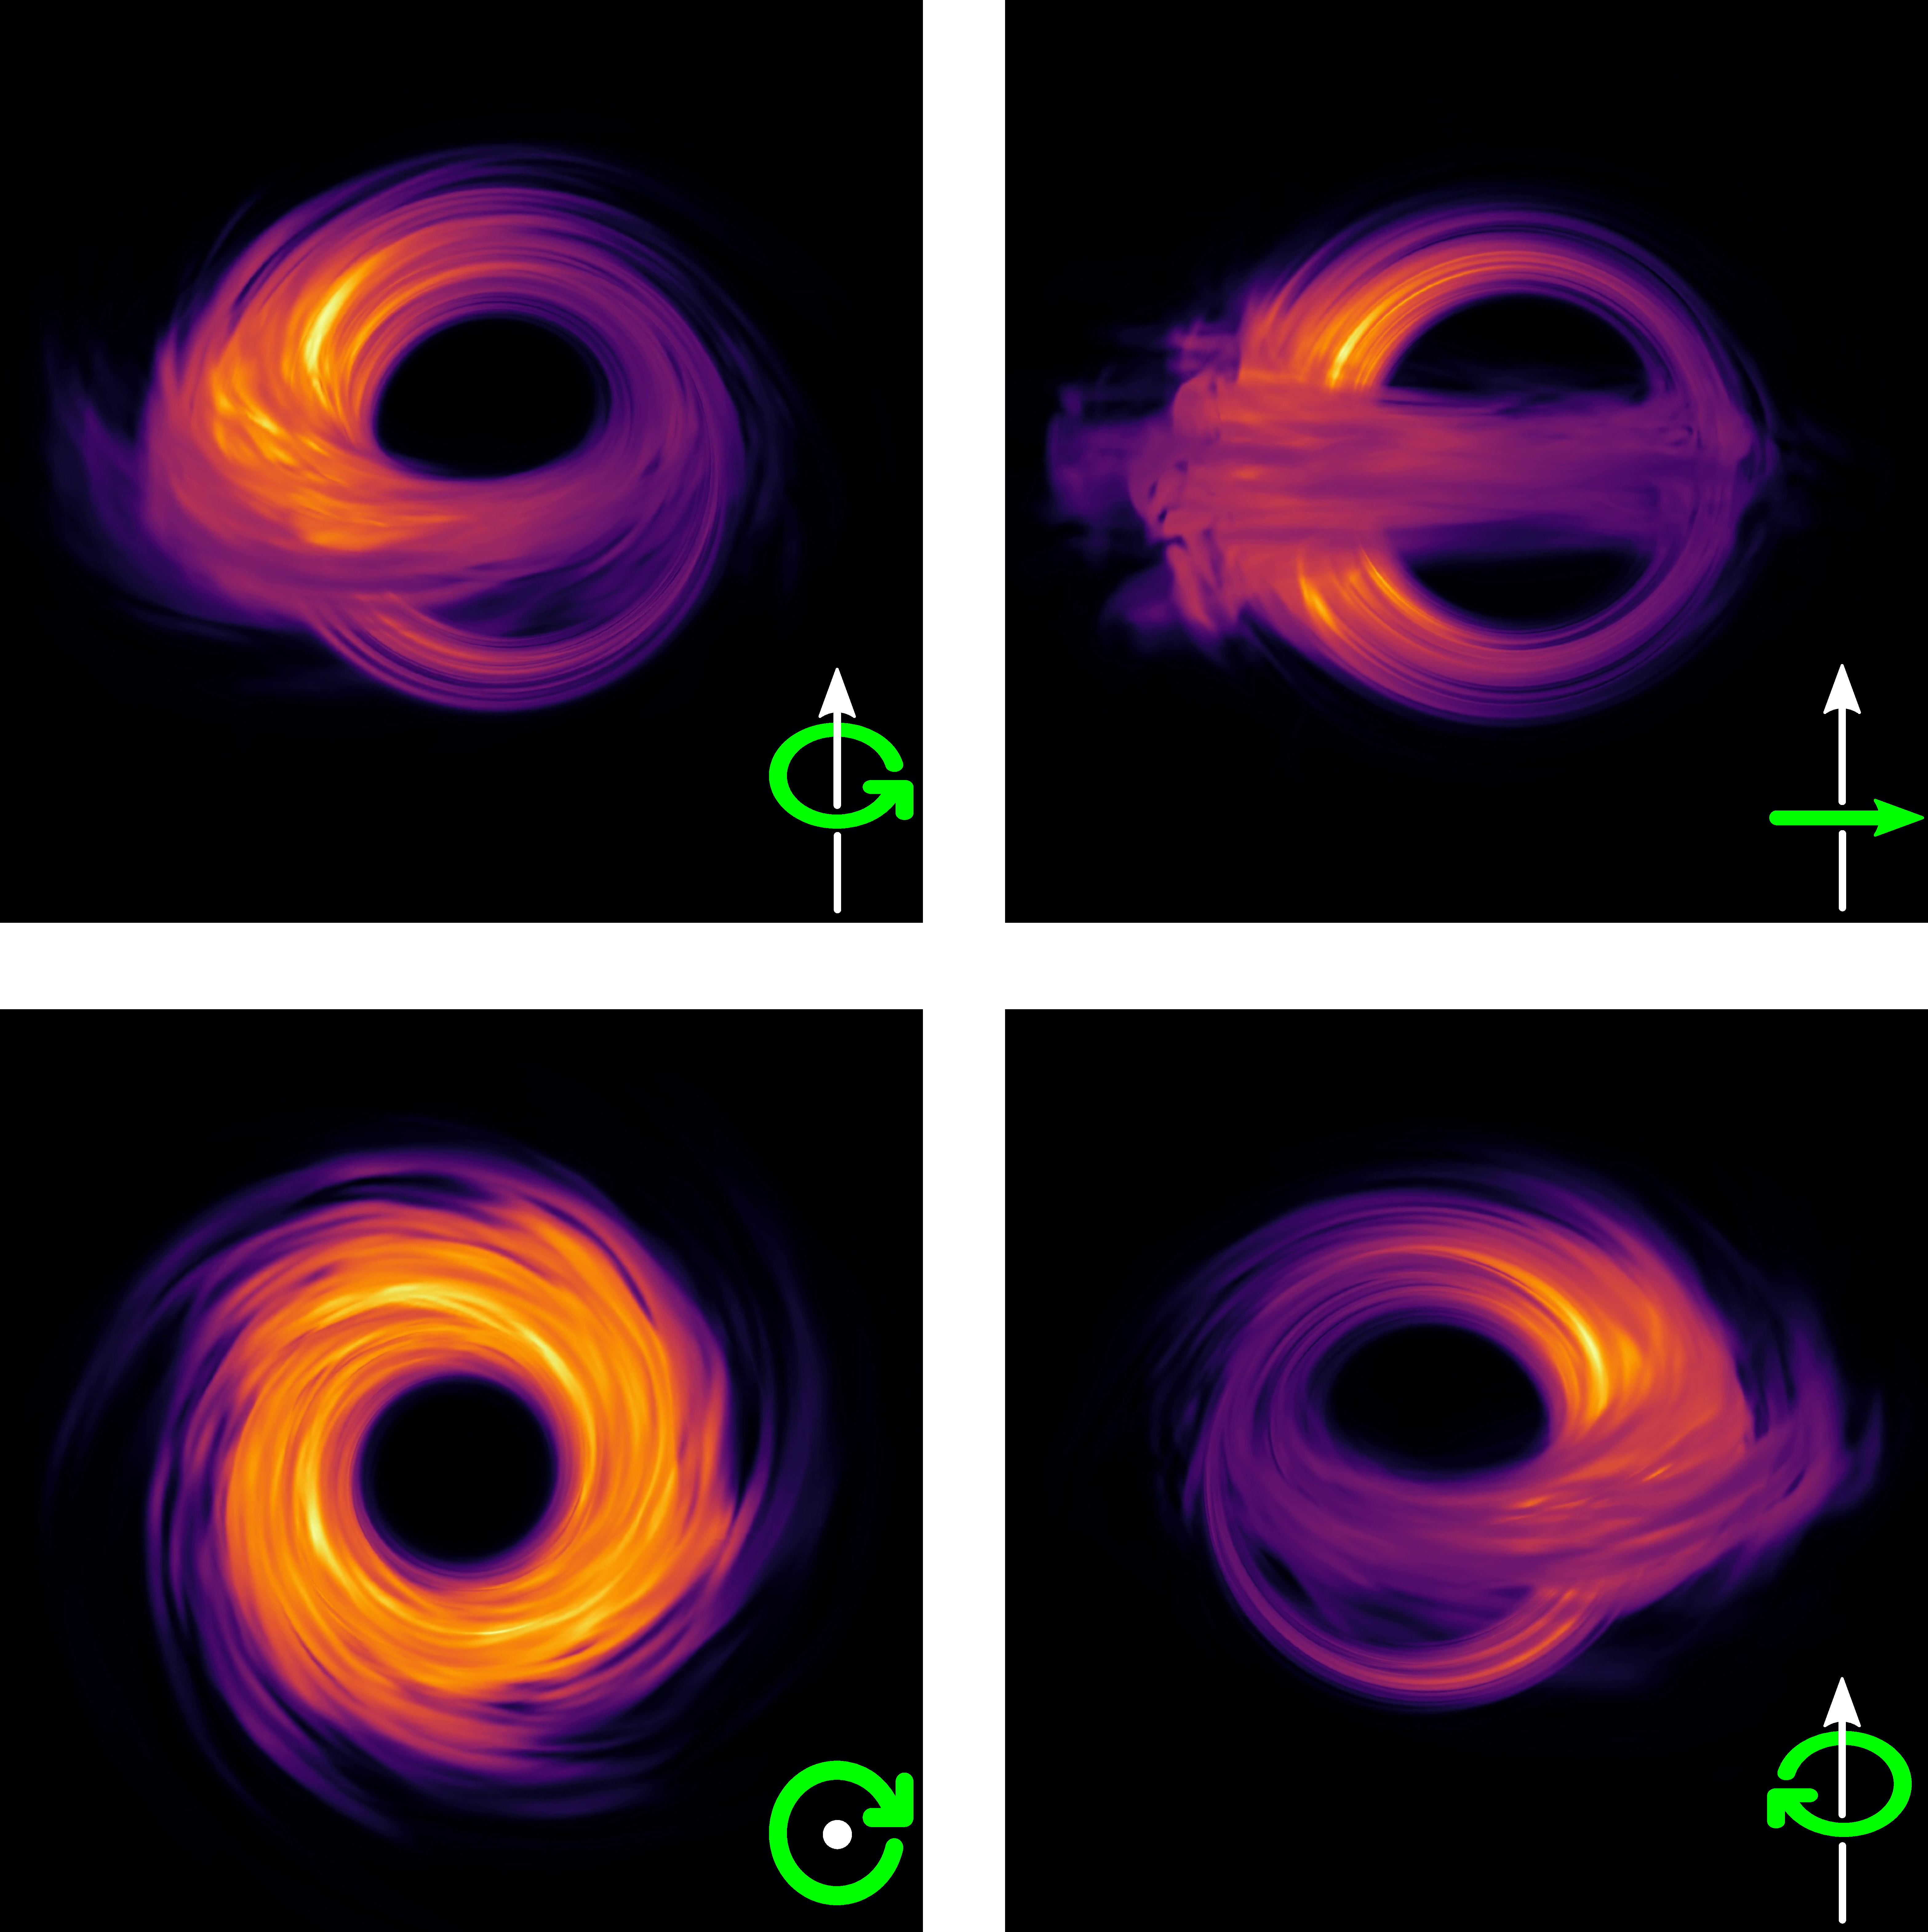
\includegraphics[width=0.88\linewidth,height=0.48\textheight,keepaspectratio]{../figs/pdf/en/fig-07-09.pdf}

% DOCX paragraph 992
\caption{\emph{Imágenes desde distintos ángulos de un disco de acreción grueso alrededor de un agujero negro en rotación. © Z. Younsi/LR.}}\label{fig:07-09}
\end{figure}

% DOCX paragraph 994
El segundo aspecto importante, visible en la figura \ref{fig:07-09} y ausente en el disco de Gargantua, es que todos los discos tienen un lado más luminoso y otro menos luminoso. La única excepción, que he incluido precisamente por serlo, está en el recuadro inferior izquierdo: corresponde a una inclinación nula, cuando observamos el disco desde el Polo Norte. La asimetría de luminosidad entre los dos lados está ligada a un fenómeno conocido, el efecto\index{Doppler!efecto} Doppler, llamado así por el físico austriaco que lo describió por primera vez en 1842. Este efecto provoca una variación de la frecuencia de una señal ondulatoria cuando la fuente está en movimiento. Dicho de otro modo, explica el cambio de frecuencia de la sirena de una ambulancia cuando se acerca o se aleja. Todos hemos oído cómo aumenta su frecuencia al aproximarse: es una señal Doppler «\emph{desplazada al azul}». Por la misma razón, la frecuencia disminuye cuando la ambulancia se aleja y produce una señal Doppler «\emph{desplazada al rojo}».\index{desplazamiento al azul (Doppler)}\index{desplazamiento al rojo (Doppler)}

% DOCX paragraph 995
Aunque el efecto Doppler\index{relativista!efecto Doppler} existe en la física clásica y lo experimentamos a menudo con fuentes que se mueven a baja velocidad respecto a nosotros, en relatividad cobra una nueva importancia: la emisión cambia no solo de frecuencia, sino también de amplitud. Más precisamente, la señal de una fuente que se acerca a velocidades próximas a la de la luz se desplaza al azul y aumenta su intensidad. Esa amplificación\index{Doppler!amplificación}, especialmente grande cuando la velocidad de la fuente se aproxima a la de la luz, suele llamarse «\emph{amplificación Doppler relativista}».

% DOCX paragraph 996
Volviendo a la figura \ref{fig:07-09}, tres de los recuadros tienen un «lado luminoso» porque en ellos hay materia girando alrededor del agujero negro: en un lado se mueve hacia nosotros y su luminosidad aumenta por la amplificación Doppler relativista\textsuperscript{\hyperlink{note:07-06}{6}}. Por la misma razón, la materia del lado opuesto se aleja y su emisión queda atenuada. Esto explica también por qué el recuadro inferior izquierdo de la figura \ref{fig:07-09} no tiene un lado luminoso y otro oscuro. Con esa inclinación, ninguna zona del disco se mueve hacia nosotros: todo el movimiento tiene lugar en un plano perpendicular a nuestra línea de visión. Por tanto, ninguna parte del disco puede ver amplificada su emisión de ese modo.

% DOCX paragraph 999
\section{Las predicciones de la teoría}\label{sec:07-theory}

% DOCX paragraph 1001
Hemos visto que la radiación emitida cerca de un agujero negro puede dar lugar a increíbles juegos de luces y sombra\index{sombra (agujero negro)}s. También hemos visto que un objeto con forma de disco, grueso o fino, que emite en la banda de radio puede tener un aspecto radicalmente distinto del que esperaríamos por nuestra experiencia del espaciotiempo plano. Nos queda por comprender cuáles deberían ser las propiedades físicas de ese objeto emisor. En otras palabras: «¿Qué le ocurre a la materia cerca de un agujero negro supermasivo?».

% DOCX paragraph 1002
Una forma sencilla de responder sería tomar cierta cantidad de materia, por ejemplo un gran cubo de agua, y verterla sobre un agujero negro en rotación. Podríamos observar qué le ocurre al caer sobre el horizonte de sucesos y usar los datos para deducir qué sucede en general con la materia que acreta un agujero negro supermasivo.

% DOCX paragraph 1003
Desde luego, sería muy cómodo y me resolvería muchos problemas, aunque probablemente me dejaría sin empleo. Por desgracia, está claro que no podemos hacerlo. La única manera, y debo insistir en «única», de responder es tomar las ecuaciones que describen el comportamiento del agua vertida sobre un agujero negro y resolverlas con potentes superordenadores\index{superordenadores}. A lo largo de mi carrera he aprendido a hacer precisamente eso de forma cada vez más realista.

% DOCX paragraph 1004
Soy consciente de que, cuando digo que me gano la vida resolviendo ecuaciones\index{ecuaciones!diferenciales} en derivadas parciales que involucran agujeros negros y estrellas de neutrones, agrando la distancia entre mis interlocutores y mí. Para evitarlo contigo, intentaré explicar en qué consiste mediante una analogía familiar. Resolver ecuaciones\index{ecuaciones!diferenciales} diferenciales para entender qué le ocurre a la materia cerca de un agujero negro se parece, con algunas diferencias, a lo que se hace para predecir el tiempo. Para muchos, una predicción meteorológica\index{predicción meteorológica} se reduce a unos iconos en una web o a un mapa con símbolos de lluvia, nubes o sol que un presentador explica en televisión. Pero esos iconos y símbolos son el resultado de cálculos complicados que se realizan varias veces al día en superordenadores\index{superordenadores} paralelos. Estos resuelven las ecuaciones de la hidrodinámica viscosa clásica, también llamadas ecuaciones de Navier-Stokes\index{ecuaciones de Navier-Stokes}\index{Navier-Stokes}, que no por casualidad son ecuaciones en derivadas parciales. Los superordenadores parten de información bastante precisa, recogida por estaciones terrestres o pilotos de líneas aéreas, sobre la velocidad del viento, la temperatura, la densidad y la composición de la atmósfera en distintos lugares. Esos datos constituyen las «condiciones iniciales» y se emplean para resolver las ecuaciones de Navier-Stokes en una región dada y con una resolución angular\index{resolución angular} determinada. Así se predicen las distribuciones futuras de velocidad, temperatura y densidad de la atmósfera. Todo este proceso se resume como «predicción del tiempo», una expresión que lo trivializa un poco. Lo que obtenemos es la solución de ecuaciones hermosas y complejas, otra muestra de que las matemáticas impregnan nuestro mundo mucho más de lo que parece a primera vista.

% DOCX paragraph 1005
Pues bien, lo que hacemos mis colegas y yo es bastante parecido, al menos en principio. También partimos de unas condiciones iniciales, por ejemplo la cantidad y la composición del agua del cubo vertido sobre el agujero negro, y resolvemos ecuaciones que nos dicen adónde va esa agua, si sigue siendo agua o se vaporiza y se convierte en plasma\index{plasma} ionizado. Nuestras ecuaciones son las de la magnetohidrodinámica\index{relativista!magnetohidrodinámica} en relatividad general, que describen la dinámica de un plasma en presencia de campos magnéticos intensos y una fuerte curvatura del espaciotiempo. No niego que son mucho más complejas que las utilizadas en las predicciones meteorológicas para calcular la cobertura de nubes en una región. Los regímenes físicos también son mucho más extremos, con las variaciones de temperatura y densidad más acusadas que puedas imaginar\textsuperscript{\hyperlink{note:07-07}{7}}.

% DOCX paragraph 1006
A pesar de estas importantes diferencias, y a riesgo de simplificar demasiado, podemos decir que nuestras simulaciones de la dinámica del plasma no son tan distintas de las predicciones meteorológicas. Está claro que no pretendemos predecir el tiempo cerca de un agujero negro, sino establecer qué le ocurre a la materia que, por distintas razones, ha acabado orbitándolo.

% DOCX paragraph 1007
Las simulaciones nos dicen que el plasma no cae sobre el agujero negro con simetría esférica: no forma una única nube esférica desde la que descienda siguiendo trayectorias radiales. Se concentra en un plano, el «plano ecuatorial», y forma un disco que gira alrededor del agujero negro mientras cae sobre él. También revelan que el disco de acreción de un agujero negro supermasivo como M87*\index{M87*} no puede ser geométricamente delgado, como en \emph{Interstellar}. Debe tener forma de rosquilla gruesa y, además, no ser ni estacionaria ni perfectamente simétrica. En el disco se desarrollan numerosos procesos e inestabilidades impulsados por los intensos campos magnéticos, responsables de la disipación y de la caída final de la materia sobre el agujero negro.

% DOCX paragraph 1008
Lo bueno de las simulaciones numéricas es que nos dan acceso a todas las propiedades del plasma, como la densidad, la velocidad, la temperatura y la presión. Podemos calcular cuánta materia cae en el agujero negro por unidad de tiempo, lo que técnicamente llamamos «tasa de acreción», o la intensidad del campo magnético cerca del horizonte de sucesos. Así descubrimos, por ejemplo, que las tasas de acreción de materia y de campo magnético no son constantes, sino «cuasiestacionarias»: fluctúan alrededor de un valor medio que permanece solo aproximadamente constante. No es muy distinto de lo que ocurre con el agua de una cascada. La cantidad que cae por unidad de tiempo es aproximadamente constante, pero fluctúa, con momentos en los que cae más y otros en los que cae menos.

% DOCX paragraph 1009
Por último, las simulaciones revelan que la acreción conduce inevitablemente a la formación de «chorro\index{relativista!chorro}\index{M87!chorro}s relativistas» en las regiones polares del agujero negro. Son zonas con muy poca materia, casi vacías, pero con campos magnéticos muy intensos. Estos son la fuerza dominante en los chorros y determinan esencialmente la dinámica del plasma. Debido a la simetría del proceso de acreción, los chorros suelen aparecer por parejas, con el campo magnético alineado en una dirección perpendicular al plano ecuatorial del disco. Las observaciones VLBI del chorro de la galaxia M87, realizadas durante décadas, han mostrado que la escasa materia del chorro se mueve prácticamente a la velocidad de la luz.\index{vacío}

% DOCX paragraph 1010
La figura \ref{fig:07-10} ofrece un ejemplo de los resultados de las simulaciones: dos imágenes de una simulación de magnetohidrodinámica en relatividad general realizada por el grupo de Fráncfort, que muestra la dinámica del plasma cerca de un agujero negro en rotación que acreta materia. El disco es grueso, turbulento y no uniforme, por lo que la tasa de acreción es solo cuasiestacionaria. En dirección perpendicular al disco emergen dos chorros relativistas, regiones con muy poca materia y campos magnéticos muy intensos, donde las partículas pueden acelerarse hasta velocidades muy elevadas.

% DOCX paragraph 1012
\begin{figure}[htbp]
\centering
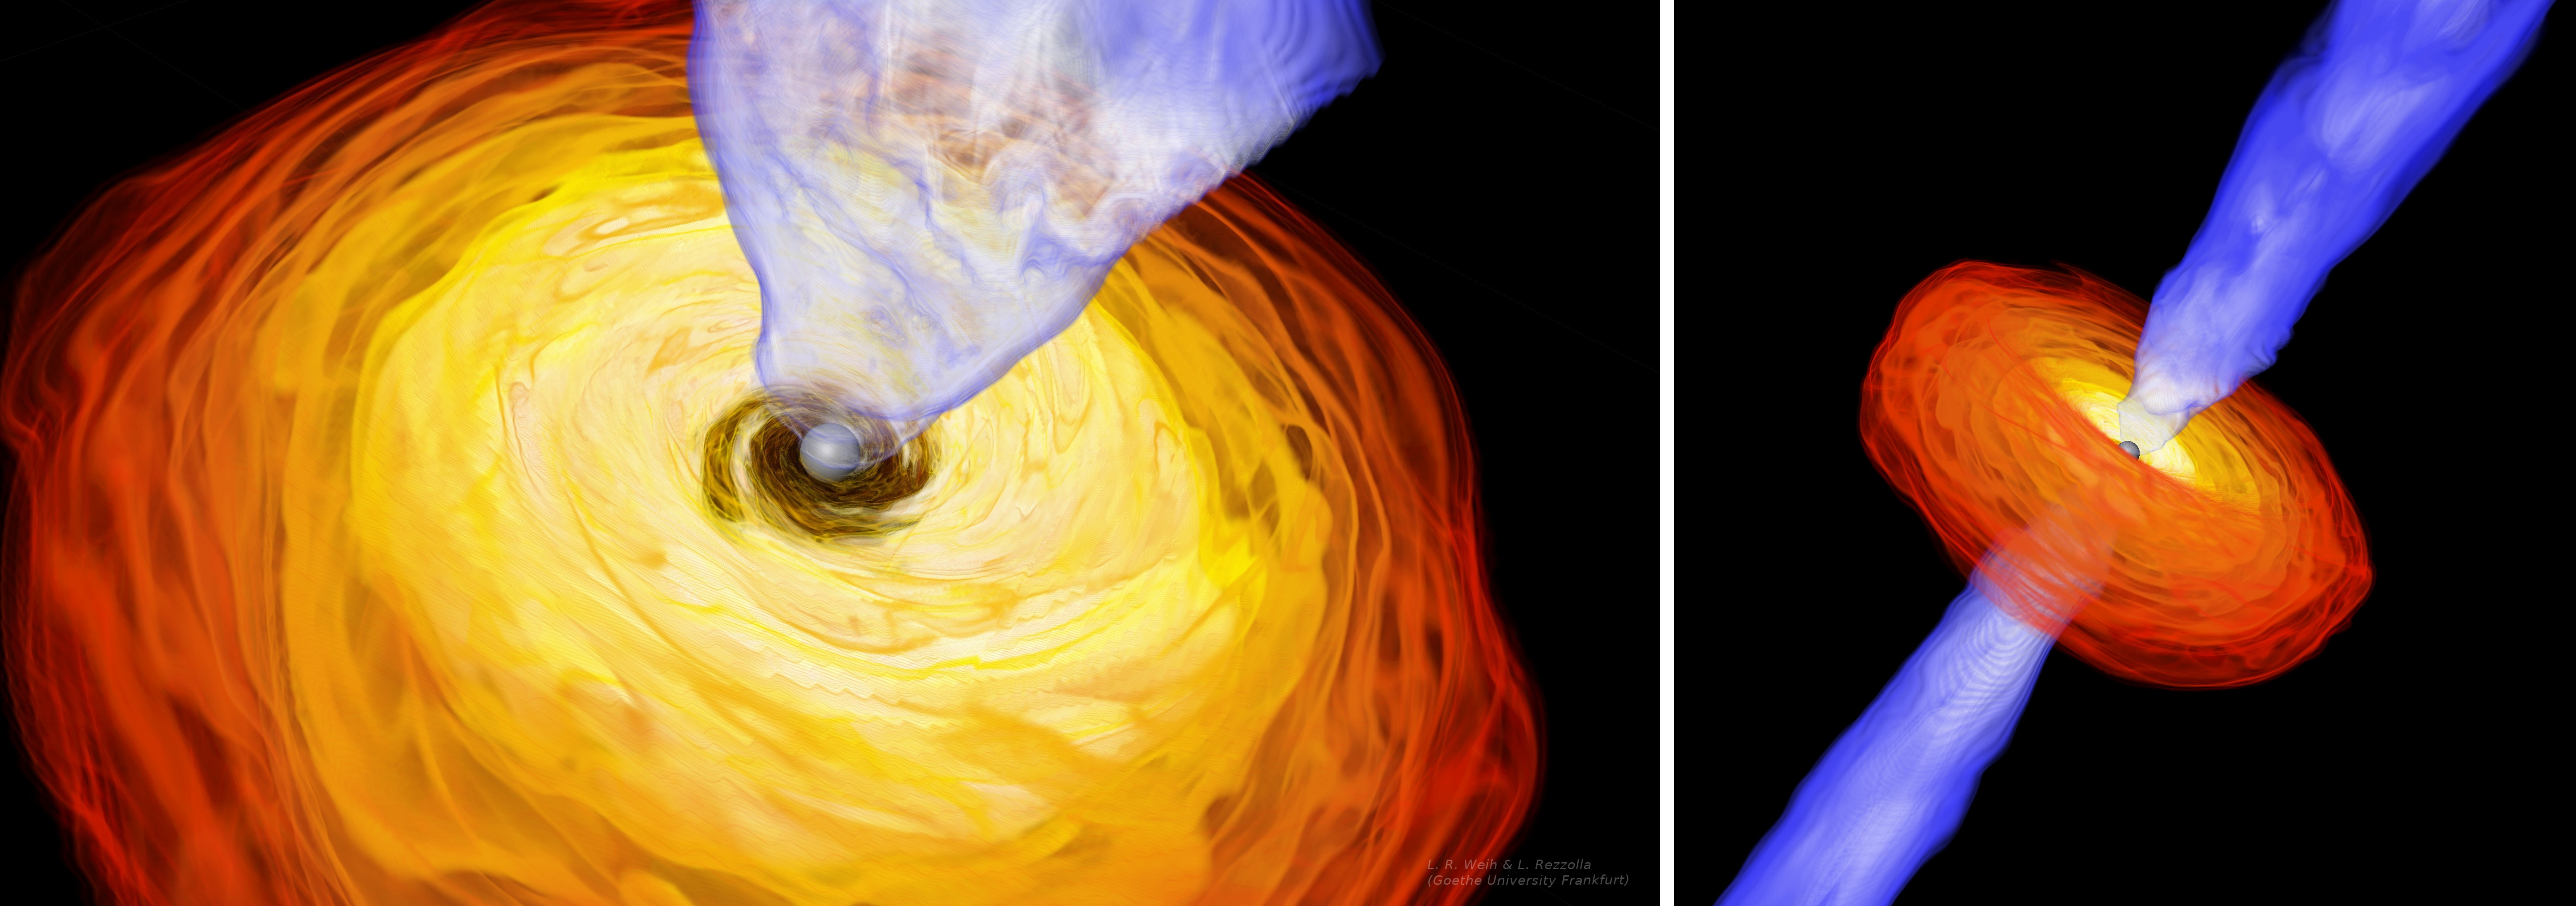
\includegraphics[width=0.88\linewidth,height=0.48\textheight,keepaspectratio]{../figs/pdf/en/fig-07-10.pdf}

% DOCX paragraph 1014
\caption{\emph{Instantáneas de una simulación numérica de la dinámica del plasma que cae sobre un agujero negro. Se distinguen un disco de acreción de materia y dos chorros relativistas. © EHT/L. Weih /LR.}}\label{fig:07-10}
\end{figure}

% DOCX paragraph 1016
Por desgracia, salvo su velocidad de propagación, sabemos muy poco sobre la composición de la materia del chorro\index{relativista!chorro}, aunque parece plausible que esté formada por partículas cargadas muy ligeras, como electrones y positrones\textsuperscript{\hyperlink{note:07-08}{8}}. Tampoco sabemos qué lanza esa materia y la acelera hasta velocidades enormes, transfiriendo cantidades inmensas de energía. Como puedes imaginar, no faltan ideas sobre el origen del lanzamiento y la aceleración de los chorros, pero todavía no hay ninguna conclusión firme\textsuperscript{\hyperlink{note:07-09}{9}}.\index{electron@electrón}

% DOCX paragraph 1017
Para añadir otro velo de incertidumbre a los muchos que envuelven los chorro\index{relativista!chorro (colimación)}\index{relativista!chorro (estabilidad)}s relativistas, tampoco comprendemos bien los procesos responsables de su colimación y estabilidad: los que permiten que conserven su forma delgada y alargada a lo largo de distancias enormes, sin romperse ni dispersarse en el espacio circundante. Son tan eficaces que el chorro de M87 permanece colimado a lo largo de una distancia que supera su sección en ocho órdenes de magnitud. Para apreciar lo que significa, pensemos en un chorro relativista como si fuera el humo que sale de un cenicero con un cigarrillo de un centímetro de diámetro. Para reproducir lo que observamos en M87, el humo tendría que permanecer colimado, sin romperse, durante unos mil kilómetros, más que la distancia entre Londres e Inverness. Queda claro que, sea cual sea su origen, el proceso de colimación es tan eficaz como extremo.

% DOCX paragraph 1018
Terminaré esta sección con una reflexión que considero muy importante para la divulgación científica, sobre todo hoy, cuando cuesta tanto distinguir la información veraz de la desinformación, la ciencia y el rigor de la ignorancia y la superficialidad.

% DOCX paragraph 1019
Es esencial insistir en la diferencia entre las imágenes producidas mediante simulaciones numéricas y las que a menudo vemos en las vistosas portadas de revistas de divulgación o en páginas web dirigidas al público. Estas últimas suelen ser «interpretaciones artísticas»: representaciones sugerentes de cómo deberían aparecer los agujeros negros según la visión de un artista. A menudo son fruto de la colaboración entre expertos en gráficos por ordenador y astrofísicos, pero, pese a las buenas intenciones, no siempre concuerdan con las leyes de la física y muchas veces solo pretenden agradarnos o estimular nuestra imaginación.\index{agujero negro!representaciones artísticas}

% DOCX paragraph 1020
En cambio, las imágenes de agujeros negros o de chorros obtenidas mediante simulaciones numéricas, que también pueden tener interés «artístico», como la figura \ref{fig:07-10}, son el resultado de resolver ecuaciones complejas. En los ejemplos de este libro, son las de la magnetohidrodinámica en relatividad general alrededor de un agujero negro en rotación. Por su propia naturaleza, estas imágenes concuerdan con las leyes de la física, pues se basan en ecuaciones que consideramos representaciones fieles de la realidad cerca de un agujero negro.

% DOCX paragraph 1021
Pero aún no nos dicen qué aspecto tendría un agujero negro supermasivo para un observador. Si queremos saber qué veríamos con unos ojos sensibles a las ondas de radio, debemos hacer un esfuerzo adicional.

% DOCX paragraph 1024
\section[De un plasma turbulento a un mapa de luz]{De un plasma turbulento a un mapa de luz}\label{sec:07-map}

% DOCX paragraph 1026
Aunque sean físicamente coherentes y puedan resultar atractivas, las imágenes de las simulaciones numéricas no revelan qué veríamos cerca de un agujero negro en rotación si nuestros ojos fueran sensibles a las ondas de radio\index{ondas!radio}. Nos dicen cómo se distribuye la \emph{materia}, no cómo ni dónde se produce la \emph{luz}. Si no hay materia, tampoco hay fuente luminosa y no puede haber imagen. Pero la presencia de materia es solo una condición necesaria: aún debemos saber cómo se distribuye la fuente luminosa y cómo produce la luz. No toda la materia presente es una fuente de luz, y no toda la que puede emitirla produce la que nosotros recibimos.

% DOCX paragraph 1027
Para hacer más comprensible esta idea, piensa en las guirnaldas de luces de colores con las que decoramos los árboles de Navidad. Imaginemos una larga secuencia de luces LED de colores, algunas estropeadas porque las últimas fiestas fueron bastante animadas y, de alguna manera, abundantes cantidades de vino espumoso acabaron rociando el árbol... Digamos que solo funciona la mitad, pero no sabemos cuáles fallan. Podemos decorar el árbol anotando la posición exacta de cada luz y después apagar las luces de casa y encender las del árbol. Como puedes imaginar, aunque conozcamos la posición de cada bombilla, aún no sabremos qué «imagen» recibiremos, es decir, qué secuencia de luces aparecerá al encenderlas. No sabemos si una luz de cierto color y en cierto lugar funcionará o no. Hay una gran variedad de combinaciones posibles, todas viables, pero solo una será la que aparezca cuando demos al interruptor...

% DOCX paragraph 1028
No es muy distinto de lo que ocurre con nuestras simulaciones del plasma alrededor de un agujero negro. Las soluciones nos dicen exactamente dónde está la materia y cuáles son sus propiedades, pero no qué partes pueden emitir luz ni con qué intensidad. Tenemos, por tanto, una complicación adicional. Además de entender qué le ocurre a la materia, debemos introducir un «\emph{modelo de emisión}» de luz en el flujo de acreción. Necesitamos un modelo matemático que vincule las propiedades del plasma más importantes para emitir luz, la densidad y la temperatura de los electrones, con un modelo físico que indique cuánta radiación se emite en la banda de radio. Volviendo al árbol de Navidad, necesitamos un modelo que nos diga qué luces funcionan, su color y la intensidad de la luz que pueden emitir.\index{electron@electrón!distribución de energía}

% DOCX paragraph 1029
Por si todo esto fuera poco, hemos visto que la luz emitida alrededor de un agujero negro puede seguir trayectorias muy extrañas. Por tanto, debemos averiguar si la radiación de una región del plasma con las condiciones adecuadas para emitirla alcanzaría realmente a un observador lejano. Tampoco podemos descartar una región poco luminosa suponiendo que no será detectable: su emisión\index{plasma!emisión} puede ser débil, pero intensificarse por efecto de lente gravitatoria\index{gravitatorio!efecto de lente} y por la amplificación relativista, hasta hacerse visible para el observador.

% DOCX paragraph 1030
Recapitulemos. Creo que ya está claro que simular el plasma\index{plasma!emisión} en acreción es solo el primer paso para obtener la imagen de un agujero negro supermasivo. El siguiente, igual de difícil y complejo, es predecir cómo emite luz la distribución de materia calculada y cómo se propaga esa luz cerca del agujero negro hasta alcanzarnos. Para ello hay que resolver el problema del «transporte de radiación\index{transporte de radiación}»: calcular la trayectoria de cada rayo en el espaciotiempo curvado y evaluar cómo interactúa con la materia que encuentra. En condiciones realistas, los rayos no viajan en el vacío\index{vacío} y sus trayectorias atraviesan inevitablemente, a menudo varias veces, la materia en acreción antes de llegar a nosotros. Según las condiciones físicas de cada punto del recorrido, la interacción con el plasma puede reducir la intensidad del rayo, si la materia lo absorbe, o aumentarla, si a la luz inicial se suma la emitida por esa porción del plasma. Calcular estas variaciones a lo largo de millones de trayectorias es tan complejo que esta etapa de la construcción teórica de la imagen solo puede completarse mediante costosas simulaciones en superordenadores\index{superordenadores} paralelos. Eso es precisamente lo que ha hecho mi grupo de investigación en Fráncfort.

% DOCX paragraph 1031
Dejaré de lado los numerosos detalles técnicos de cómo se resuelve en la práctica el transporte de radiación\index{transporte de radiación}, que no son especialmente relevantes aquí. En la figura \ref{fig:07-11} he reunido esquemáticamente las tres fases principales del proceso que conduce a construir una \emph{imagen sintética\index{imagen sintética}}, es decir, puramente teórica, de un agujero negro supermasivo que acreta materia.

% DOCX paragraph 1033
\begin{figure}[htbp]
\centering
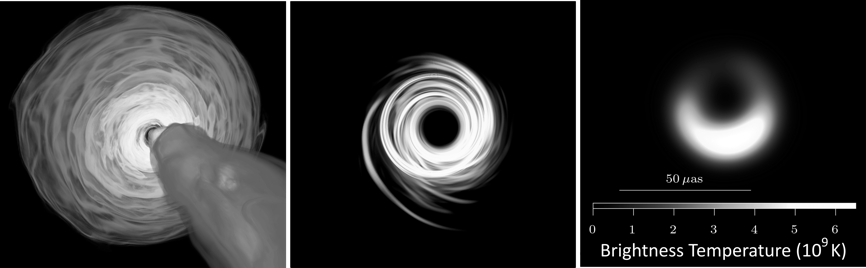
\includegraphics[width=0.88\linewidth,height=0.48\textheight,keepaspectratio]{../figs/source/en/fig-07-11.png}

% DOCX paragraph 1035
\caption{\emph{Las tres fases de la construcción de una imagen sintética. © L. Weih/C. Fromm/Z. Younsi/LR.}}\label{fig:07-11}
\end{figure}

% DOCX paragraph 1037
El recuadro izquierdo muestra el resultado de una simulación de la dinámica del plasma: su distribución en el disco de acreción y los campos magnéticos del chorro (véase también la figura \ref{fig:07-10}). El recuadro central muestra la emisión en la banda de radio, concretamente a 230 GHz, calculada a partir de esas distribuciones. Es decir, muestra cómo veríamos la materia del recuadro izquierdo si nuestros ojos fueran sensibles a las ondas de radio. Por último, como la imagen sintética\index{imagen sintética} del recuadro central de la figura \ref{fig:07-11} es \emph{ideal}, correspondiente a un instrumento perfecto y sin ruido\index{ruido}, el recuadro derecho muestra cómo aparecería realmente la emisión al registrarla con una red de radiotelescopios conectados mediante VLBI, con una resolución alta, pero finita. Las tres imágenes se han obtenido desde un ángulo que refleja aquel desde el que creemos estar observando M87*\index{M87*}.

% DOCX paragraph 1038
La figura \ref{fig:07-11} invita a varias reflexiones. Primero, al pasar del recuadro izquierdo al central, vemos que no toda la materia en acreción contribuye a la emisión de radio: en esta imagen concreta, por ejemplo, el chorro contribuye poco. Además, la máxima intensidad no siempre corresponde a las zonas de mayor densidad, aunque buena parte de la emisión suele proceder de las regiones internas del disco, que son también las más densas.

% DOCX paragraph 1039
Segundo, la imagen central combina todas las contribuciones luminosas producidas cerca del agujero negro que, tras desviarse y amplificarse, pueden alcanzar a un observador lejano. Aunque la mayor parte de la luz procede del disco, también contribuye el chorro\index{relativista!chorro (que se acerca)}\index{relativista!chorro (que se aleja)} que se mueve hacia nosotros, el «chorro que se aproxima», e incluso el que se aleja, el «chorro que retrocede». Como hemos visto, la luz emitida en dirección opuesta a nuestra línea de visión puede desviarse y alcanzarnos si la materia en acreción es «ópticamente delgada» en esa banda de radio, es decir, esencialmente transparente. Si fuera «ópticamente gruesa», la luz del chorro que retrocede sería absorbida y el chorro resultaría invisible.

% DOCX paragraph 1040
Por último, el recuadro derecho recuerda que la resolución alcanzable con la tecnología actual, aun siendo la mayor conseguida hasta ahora, está lejos de la que querríamos y de la que nos permitiría extraer mucha información de la imagen de un agujero negro. Pero Roma no se hizo en un día, y el proceso no termina con los resultados del EHT de 2019. Al contrario: la imagen de la figura \ref{fig:07-01} debe considerarse el comienzo de un proceso que tardará décadas en desarrollarse por completo.

% DOCX paragraph 1041
Antes de terminar esta sección, volvamos a la analogía entre la materia acretada por un agujero negro y el caudal de una cascada. El movimiento de la materia alrededor del agujero negro es turbulento y, por tanto, irregular, aunque tenga propiedades estadísticas precisas, como valores medios y fluctuaciones de amplitud casi constante. Si la materia se mueve de forma turbulenta y fluctuante, también lo hará su emisión de luz. La consecuencia es tan sencilla como importante: no puede haber una imagen \emph{única} y \emph{estática} de M87*\index{M87*}. Debe ser dinámica y fluctuante, para representar el estado de la materia que lo rodea en un momento dado.

% DOCX paragraph 1042
Si lo piensas, no debería sorprenderte. Imagina que tomas una serie de fotos de una montaña en distintos momentos, como al hacer un vídeo con la técnica \emph{time-lapse}. Las imágenes serán muy parecidas, pero ninguna será idéntica a la anterior: quizá se haya movido una nube o haya cambiado un poco la iluminación. Lo que ocurre en nuestras simulaciones, y por tanto en las observaciones de radio, no es muy distinto cuando intentamos obtener una imagen de M87*\index{M87*}. La distribución de la materia cambia continuamente, y lo mismo sucede con la emisión de radio. La imagen estará inevitablemente sujeta a variabilidad\index{variabilidad}, como cuando intentamos fotografiar a un niño pequeño y revoltoso que no hace caso de nuestras peticiones de que se quede quieto. Todos sabemos que la única forma de obtener fotos que no salgan movidas es usar un tiempo de exposición menor que el tiempo típico en el que cambia el sujeto. ¡Tenemos que disparar más rápido de lo que se mueve!

% DOCX paragraph 1043
Quizá te preguntes: «¿En qué escala de tiempo varía la emisión de M87*\index{M87*}?». Aunque refleja una dinámica muy compleja, la respuesta es sencilla: depende de la masa del agujero negro. Más precisamente, puede asociarse al tiempo aproximado necesario para recorrer una órbita\index{orbita@órbita} circular a su alrededor. En el caso más simple, un agujero negro sin rotación y una órbita cercana al anillo de luz, ese tiempo es \(\tau\sim(3GM/c^{3})\). La estimación tiene en cuenta que basta considerar una parte de la órbita y que esta puede situarse a radios menores que el del anillo de luz.

% DOCX paragraph 1044
Si calculamos ese tiempo para la masa estimada de M87*\index{M87*}, 6\,500 millones de masas solares, obtenemos una escala de variabilidad\index{variabilidad} del orden de 24 horas. Así, aunque la fuente de radiación en torno a M87* fluctúe de forma intrínseca, parecerá casi estática si usamos exposiciones de menos de un día. Como las observaciones del EHT se realizaron durante unas 8 a 10 horas, el tiempo desde que M87* aparece para el primer telescopio, en Francia, hasta que desaparece para el último, en Hawái, las imágenes VLBI son esencialmente estáticas. Cualquier variación debería ser pequeña y aparecer solo al comparar días distintos, ¡que es precisamente lo que han mostrado las observaciones!

% DOCX paragraph 1045
Por desgracia, la emisión de Sgr A* no es cuasiestacionaria de ese modo: su masa es casi mil veces menor que la de M87*\index{M87*} y su variabilidad\index{variabilidad} esperada es del orden de unos pocos minutos. En esas condiciones, las observaciones VLBI se parecerían a una película breve e incompleta, mucho más difícil de analizar e interpretar. El EHT está actualmente en la fase final del análisis de las observaciones VLBI de Sgr A*, cuya imagen debería publicarse antes del verano de 2022.

% DOCX paragraph 1046
Cerraré esta sección con una pregunta que quizá te hayas planteado: «¿Deberíamos tener en cuenta los cambios en la masa del agujero negro debidos a la acreción de materia durante las observaciones?».

% DOCX paragraph 1047
La pregunta es interesante y la respuesta sencilla y categórica: no, no tenemos que preocuparnos. Los tiempos de variación de la masa de un agujero negro supermasivo son enormes comparados con la duración de las observaciones. Para entenderlo, recuerda que las observaciones de M87*\index{M87*} nos han permitido estimar que su masa aumenta en una sola masa solar durante cuatrocientos años de acreción. Como la masa total de M87* es de miles de millones de masas solares, en diez millones de años aumentará, como mucho, en una parte por millón. No es muy distinto de lo que ocurre al fotografiar la montaña para un vídeo \emph{time-lapse}. Sabemos que la montaña cambiará mientras tomamos las fotos: la erosión la desmenuzará de forma lenta e inexorable, y en unos diez millones de años gran parte acabará en el mar. Pero, como esos cambios son minúsculos, no pensamos en ellos al hacer nuestro vídeo de la hermosa montaña...

% DOCX paragraph 1053
\section{Las imágenes de M87*}\label{sec:07-images}\index{M87*}

% DOCX paragraph 1055
He insistido en que simular la dinámica del plasma\index{plasma} no es conceptualmente muy distinto de lo que hacen los meteorólogos al predecir el tiempo. Pero hay una diferencia importante: las predicciones meteorológicas abarcan una ventana relativamente estrecha del futuro, de unas horas a unos días, tras la cual pierden fiabilidad. Nuestras simulaciones, en cambio, cubren periodos mucho más largos, del orden de una década.

% DOCX paragraph 1056
Esto puede sorprenderte y suscitar una pregunta obvia: «¿Por qué demonios simular diez años si las observaciones duran menos de un día?». Lo hacemos para construir una estadística fiable de los posibles estados de acreción del agujero negro. Así, después de observarlo con VLBI y reconstruir su imagen, podemos compararla con una extensa «biblioteca\index{imagen sintética!biblioteca}» de imágenes sintéticas de un agujero negro supermasivo en acreción. Por volver a una analogía anterior, no tomamos una sola foto de la montaña, sino varias al día durante diez años. Esperamos que, si algún día encontramos una foto borrosa que pudiera ser de una montaña, nuestro catálogo de montañas en distintas condiciones permita averiguar si lo es y quizá deducir sus propiedades.

% DOCX paragraph 1057
Siguiendo esa lógica, los científicos del EHT, y en particular el grupo de Fráncfort, han emprendido la campaña más extensa y sistemática de simulaciones numéricas de agujeros negros en acreción realizada hasta ahora. Queríamos construir la descripción más amplia y completa de las condiciones físicas del plasma que cae sobre un agujero negro. Con códigos numéricos complejos y sofisticados y numerosos superordenadores\index{superordenadores} paralelos, realizamos muchas simulaciones de muy alta resolución angular\index{resolución angular}, que abarcan los principales escenarios en los que un agujero negro supermasivo puede acretar materia.

% DOCX paragraph 1058
En particular, variamos uno o varios de los siguientes parámetros:

% DOCX paragraph 1059
\begin{itemize}
\item \emph{El espín del agujero negro}. Consideramos tanto agujeros negros sin rotación como otros que giran muy deprisa.

% DOCX paragraph 1060
\item \emph{El sentido de rotación del plasma respecto al agujero negro}. Estudiamos plasma que corrota o contrarrota con él.

% DOCX paragraph 1061
\item \emph{La intensidad del campo magnético}. Exploramos dos tipos de discos de acreción que difieren en la tasa de acreción que pueden producir, pequeña o grande.
\end{itemize}

% DOCX paragraph 1062
Quizá hayas advertido que no he mencionado la masa como un parámetro variable: todos los agujeros negros considerados tenían exactamente la misma masa. Esto fue posible porque, aunque la masa desempeña un papel muy importante, puede eliminarse fácilmente como factor del problema. Todas las magnitudes calculadas pueden reescalarse de forma adecuada, de modo que una misma simulación describa la acreción sobre un agujero negro de una masa solar o de mil millones de masas solares.

% DOCX paragraph 1063
No tiene sentido detallar aquí las numerosas simulaciones, cada una de las cuales permitió producir cientos de imágenes sintéticas distintas. Basta decir que abarcaron una gran variedad de escenarios. En algunos, el disco de acreción es muy luminoso; en otros, su emisión es muy débil. A veces el disco termina muy cerca del horizonte, como suele ocurrir con agujeros negros de espín elevado y plasma en corrotación. En otros casos termina muy lejos: esto sucede con agujeros negros de espín elevado, pero con plasma en contrarrotación.\index{imagen sintética}

% DOCX paragraph 1064
Para ampliar aún más la variedad de imágenes sintéticas, acompañamos cada simulación de distintos modelos de emisión que especificaban las propiedades energéticas de los electrones responsables de la radiación de radio. Así, una misma simulación produjo muchas realizaciones adicionales de las imágenes sintéticas, con una secuencia nueva para cada modelo de emisión\index{electron@electrón!modelo de emisión}.

% DOCX paragraph 1065
En su esfuerzo por interpretar teóricamente las observaciones y extraer toda la información posible, no sorprende que el EHT produjera, en poco más de seis meses, nada menos que \emph{60\,000 imágenes sintéticas}. Estas abarcan la mayoría de las configuraciones posibles de un agujero negro en acreción. La biblioteca resulta aún más impresionante si tenemos en cuenta que no sabíamos cómo estaba orientado M87*\index{M87*} respecto a nuestra línea de visión. Esa era, precisamente, una de las cosas que queríamos averiguar. Por tanto, cada imagen sintética\index{imagen sintética} podía generar cientos de imágenes adicionales con solo cambiar los dos ángulos de rotación.

% DOCX paragraph 1066
Desde un punto de vista conceptual, cada una de esas 60\,000 imágenes es una realización plausible y físicamente coherente del aspecto de un agujero negro supermasivo en acreción, observado con una red de radiotelescopios conectados mediante VLBI. Pero también es posible que ninguna de las 60\,000 imágenes \emph{sintéticas} corresponda a alguna de las cuatro imágenes \emph{observadas} que el EHT reconstruyó a partir de los datos de los días 5, 6, 10 y 11 de abril de 2017, y que reproduzco a continuación.\index{imagen sintética}

% DOCX paragraph 1068
\begin{figure}[htbp]
\centering
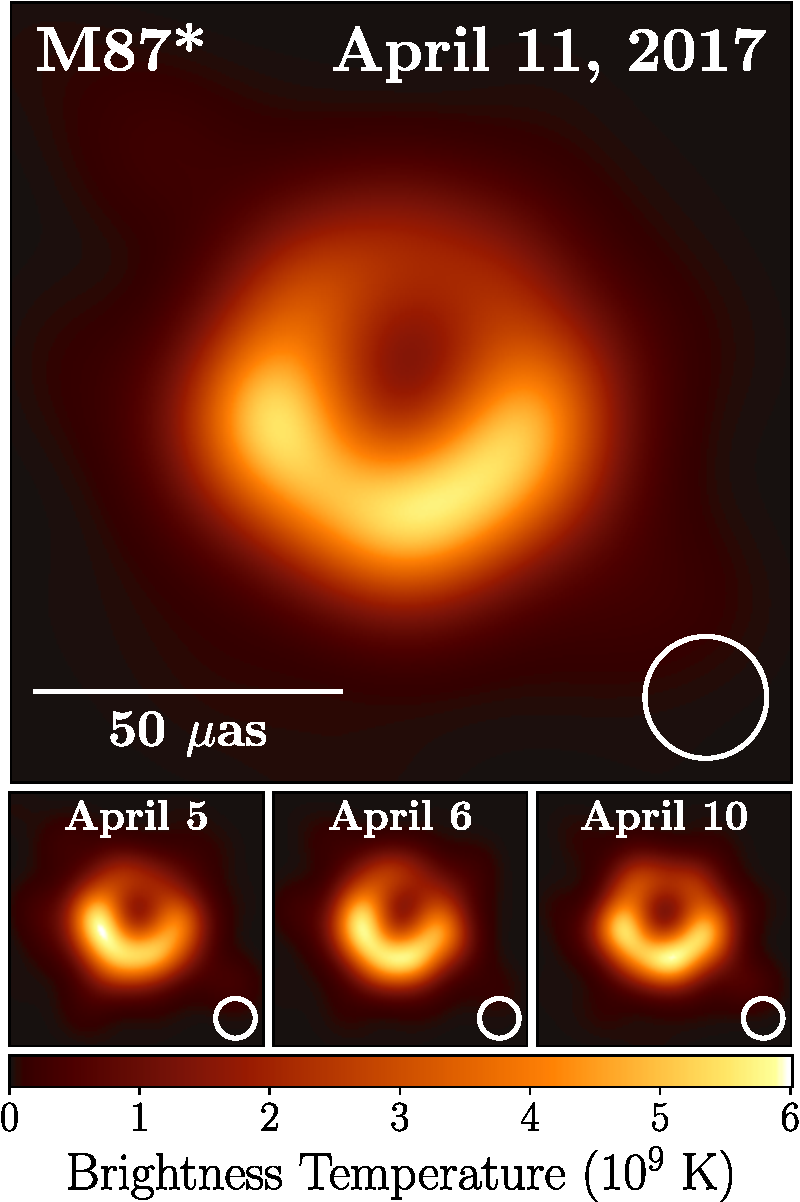
\includegraphics[width=0.88\linewidth,height=0.48\textheight,keepaspectratio]{../figs/pdf/en/fig-07-12.pdf}

% DOCX paragraph 1070
\caption{\emph{Cuatro imágenes de M87*\index{M87*} tomadas en distintos días de abril de 2017 por la colaboración EHT, a una radiofrecuencia de 230 GHz. © The EHT Collaboration.}}\label{fig:07-12}
\end{figure}

% DOCX paragraph 1072
Como muestra la figura \ref{fig:07-12}, y como era de esperar, las imágenes varían algo de un día a otro, pero sus propiedades básicas son, en conjunto, bastante «robustas».

% DOCX paragraph 1075
\section{Como una aguja en un pajar}\label{sec:07-needle}

% DOCX paragraph 1077
Permíteme recapitular la larga secuencia de sucesos y argumentos que hemos recorrido. En abril de 2017, tras meses de preparación, el EHT realizó observaciones VLBI de M87*\index{M87*} y, después de más de un año trabajando con los datos, reconstruyó cuatro imágenes observadas. Mientras tanto, entre finales de 2018 y principios de 2019, emprendió una gran campaña de simulaciones teóricas para predecir el aspecto de un agujero negro supermasivo rodeado de plasma en acreción\index{plasma!en acreción}, y produjo 60\,000 imágenes sintéticas. Aún no he descrito el último paso del análisis, la pieza que falta en el rompecabezas de la primera foto de un agujero negro. Consistía en averiguar cuáles de las 60\,000 imágenes sintéticas correspondían a las cuatro observadas, para comprender por fin qué nos decían las observaciones. Aunque lógicamente parezca sencillo, era como buscar la proverbial aguja en un pajar... Por suerte, pudimos recurrir a los ordenadores para superar este último desafío.

% DOCX paragraph 1078
Hay algoritmos matemáticos sofisticados que permiten resolver problemas de este tipo, muy complejos y con múltiples parámetros posibles, aprovechando la potencia de cálculo de grandes superordenadores\index{superordenadores}. Podemos omitir los detalles técnicos de algoritmos con nombres tan sugerentes como «Montecarlo mediante cadenas de Markov\index{algoritmo!cadena de Markov}» o «genéticos\index{algoritmo!genético}». Solo diré que encuentran soluciones óptimas, o casi óptimas, a problemas con grandes cantidades de datos que dependen de muchos parámetros. Una vez encontrado el «mejor ajuste» entre los datos y el modelo, cuantifican la probabilidad de que un parámetro esté dentro de cierto intervalo. Así pudimos comparar las cuatro imágenes observadas con las sintéticas y determinar la probabilidad de que un parámetro, por ejemplo la masa o el espín del agujero negro, estuviera en un intervalo dado.

% DOCX paragraph 1079
Para entender mejor cómo funciona en la práctica este proceso de comparación, hagamos otro experimento mental. Imagina que estás en un estadio con 60\,000 espectadores que esperan ansiosos el comienzo de un partido importante. Al entrar, te parece ver a una persona amiga a la que has perdido entre la multitud que se agolpaba en la entrada. No sabes con certeza si era esa persona ni, de serlo, si se encuentra ahora en el estadio. Por suerte, llevas contigo una foto reciente, aunque muy borrosa, de esa persona. La seguridad del estadio utiliza un circuito cerrado de televisión cuyas cámaras fotografían a cada espectador al entrar. Te acercas al amable encargado del sistema de vigilancia y le pides que compare tu foto borrosa con las fotos de alta resolución tomadas en la entrada por las cámaras fijas. El sistema de vigilancia utilizará algoritmos de Montecarlo mediante cadenas de Markov o algoritmos genéticos para encontrar la mejor coincidencia entre las imágenes tomadas en la entrada y la de la persona que buscas. En la práctica, se emplearán técnicas de reconocimiento facial que descomponen un rostro humano en sus rasgos principales: la distancia entre los ojos, la posición de la nariz respecto a ellos, el tamaño de la boca, etcétera. En esencia, cada retrato se descompone en una serie de parámetros, básicamente \emph{N} números, uno por cada rasgo facial. Los algoritmos comparan la secuencia de \emph{N} números correspondiente a tu foto borrosa con los \emph{N} números de cada una de las 60\,000 imágenes de la biblioteca de retratos. La parte «inteligente» del algoritmo consiste en buscar la mejor coincidencia sin recorrer toda la biblioteca, sino «moviéndose» de forma eficiente por el espacio de secuencias de \emph{N} números y concentrándose solo en aquellas para las que ya hay una buena coincidencia. Así la búsqueda resulta más sencilla y, sobre todo, más rápida.

% DOCX paragraph 1080
La figura \ref{fig:07-13} ofrece una representación esquemática de este proceso. La imagen superior izquierda es la foto borrosa de la persona que buscas, que, al menos desde un punto de vista lógico, es similar a la figura \ref{fig:07-01}. La imagen superior derecha muestra, como comparación, la biblioteca de retratos, compuesta, para ser precisos, por 54\,200 imágenes.\textsuperscript{\hyperlink{note:07-10}{10}} Las dos filas inferiores muestran diez fotos de la biblioteca que los algoritmos han seleccionado como las más parecidas a la imagen de referencia. Desde un punto de vista matemático, son las que han obtenido las «puntuaciones» más altas al comparar los parámetros asociados al rostro de esa persona.

% DOCX paragraph 1081
El proceso de comparación de imágenes de la figura \ref{fig:07-13}, conceptualmente muy similar al que realizamos con M87*\index{M87*}, nos enseña algunas lecciones importantes. En primer lugar, revela que la operación matemática de proyectar la imagen de referencia sobre el espacio representado por la biblioteca de imágenes de los espectadores del estadio no es única; es decir, la proyección es degenerada. Dicho de una manera quizá más comprensible, el proceso de comparación revela que, en general, hay varios candidatos. En nuestro caso hay al menos diez, aunque podrían ser más o menos según la tolerancia del algoritmo, que, con una puntuación prácticamente igual, cumplen todos los criterios impuestos para encontrar una imagen «suficientemente parecida» a la de la persona que buscas. Nada sorprendente: como en el caso del reloj de pared, mientras la información de la que disponemos sea limitada y se restrinja a las observaciones, es casi inevitable que haya varias respuestas posibles.

% DOCX paragraph 1082
\begin{figure}[htbp]
\centering
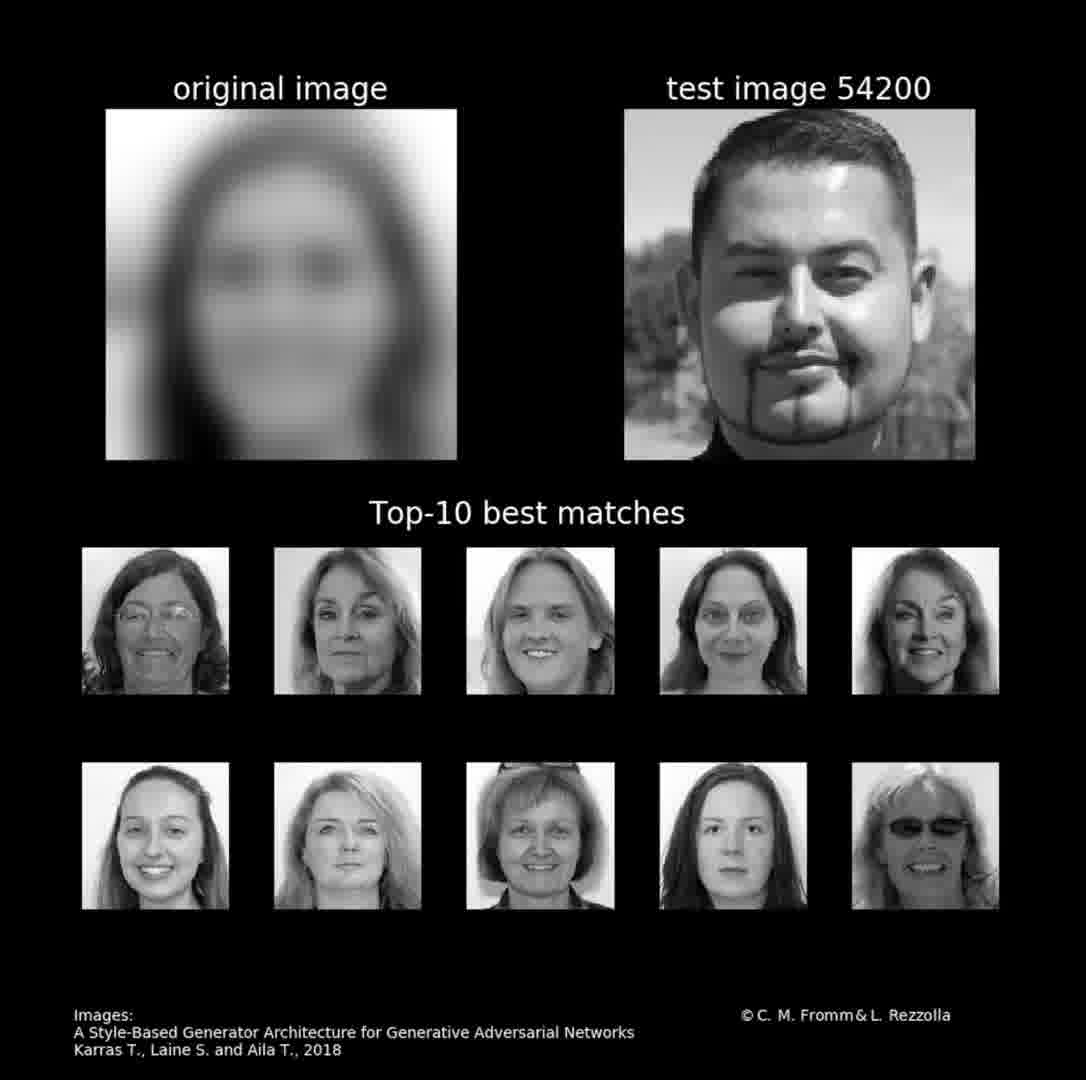
\includegraphics[width=0.88\linewidth,height=0.48\textheight,keepaspectratio]{../figs/source/en/fig-07-13.jpg}

% DOCX paragraph 1084
\caption{\emph{Proceso de comparación de imágenes. © C. Fromm/LR. Images: T. Karras, S. Laine, T. Aila.}}\label{fig:07-13}
\end{figure}

% DOCX paragraph 1086
En segundo lugar, aunque hay buenos ajustes, parece que esa persona no está en el estadio, ya que ninguna de las mejores imágenes parece corresponderse con la de referencia, a pesar de que algunas se acercan bastante. Fíjate en que he escrito «parece», porque estos algoritmos de reconocimiento facial solo miden la probabilidad de una determinada coincidencia, y esta nunca es del 100\% a menos que dispongamos de imágenes «perfectas»: sin ruido o, si se prefiere, perfectamente nítidas y de una resolución muy elevada. También en la comparación entre las imágenes observadas de M87*\index{M87*} y las sintéticas, el resultado del ajuste se mide en términos de probabilidades. Aunque nos hemos esforzado al máximo por crear una imagen sintética\index{imagen sintética} lo más cercana posible a la realidad, esta siempre es más compleja de lo que podemos representar con nuestras simulaciones. Por tanto, es perfectamente plausible y científicamente aceptable que ninguna de los cientos de miles de imágenes producidas sintéticamente se corresponda «exactamente» con la observada.

% DOCX paragraph 1087
Las propiedades de las diez imágenes con mejor ajuste de las filas inferiores nos dan la tercera y última lección. La selección que ofrecen los algoritmos revela que la persona que buscas pertenece a una clase particular de seres humanos: las mujeres de pelo largo. En efecto, todas las personas de las imágenes con mejor ajuste son mujeres. Aunque en el estadio también había hombres con pelo largo, el algoritmo de reconocimiento facial no eligió a ninguno, lo que revela que tu amiga tiene el pelo largo y, además, es una mujer.

% DOCX paragraph 1088
Por supuesto, podrías objetar que este resultado es trivial: ya sabes que tu amiga es una mujer y que tiene el pelo largo. Sin embargo, por lo que respecta a la imagen de M87*\index{M87*}, no sabíamos a qué clase de objeto se refería. Por tanto, ¡solo con estudiar las propiedades de los mejores ajustes podíamos aprender mucho sobre la imagen, incluso sin haber encontrado un ajuste perfecto!

% DOCX paragraph 1089
Regresemos ahora a lo que realmente hemos hecho con el EHT y M87*\index{M87*}, y dejemos de lado las amistades y los sucesos del estadio. La figura \ref{fig:07-14} lo ilustra mostrando la excelente coincidencia entre la imagen de M87* observada el 11 de abril de 2017, en el panel izquierdo, y una imagen sintética\index{imagen sintética} desenfocada de forma apropiada para tener en cuenta el ruido\index{ruido} experimental, en el panel derecho.

% DOCX paragraph 1090
\begin{figure}[htbp]
\centering
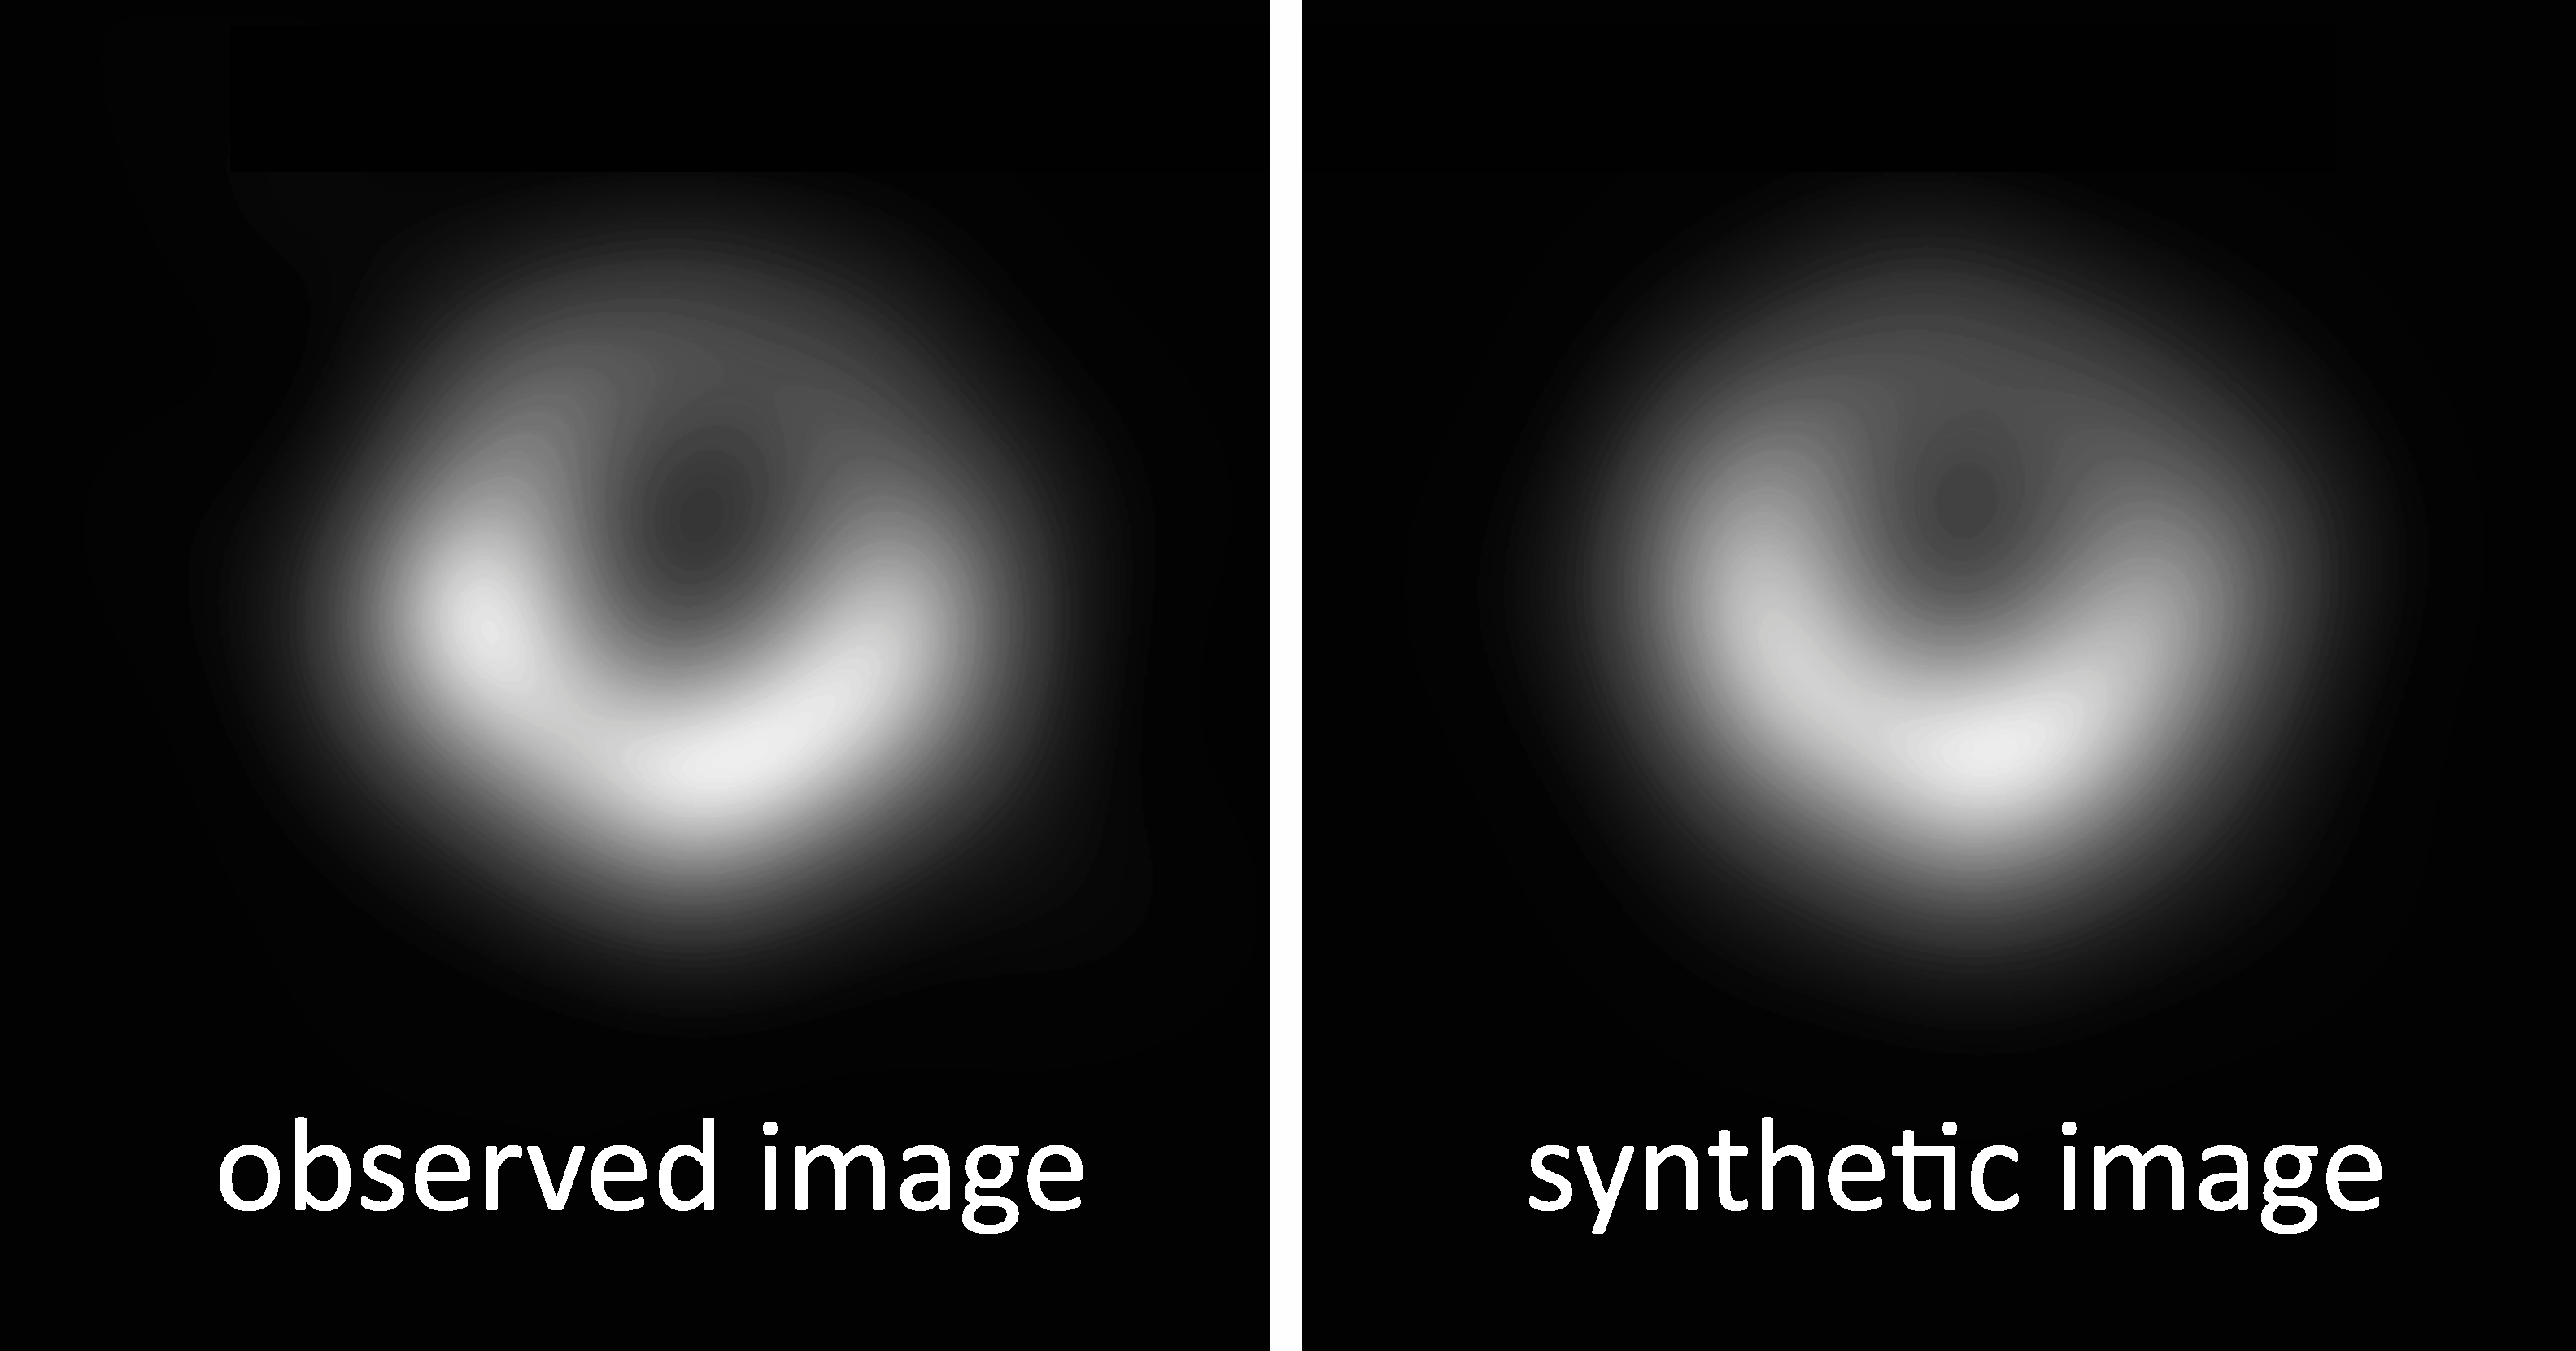
\includegraphics[width=0.88\linewidth,height=0.48\textheight,keepaspectratio]{../figs/pdf/en/fig-07-14.pdf}

% DOCX paragraph 1092
\caption{\emph{Ejemplo del excelente ajuste entre una imagen observada de M87*\index{M87*} y una imagen sintética adecuadamente deteriorada. © The EHT Collaboration/C. Fromm/LR.}}\label{fig:07-14}
\end{figure}

% DOCX paragraph 1094
Creo que está claro que la similitud entre ambas es impresionante. De hecho, la puntuación que los algoritmos han asignado a la imagen de la derecha está entre las más altas de los cientos de miles de imágenes sintéticas producidas.

% DOCX paragraph 1095
La imagen de la derecha es una predicción completamente teórica. Se obtuvo mediante simulaciones de la dinámica del plasma y empleando un modelo preciso de la emisión de radiación. De ahí que conozcamos todas las características del objeto que hay detrás de esa imagen: la masa y el espín del agujero negro, la inclinación respecto al observador, la temperatura y la distribución de energía de los electrones, etcétera. Por lógica, podríamos creer que también lo sabemos todo sobre la imagen de la izquierda. ¡Pero esta lógica, aunque sencilla, por desgracia es errónea! La razón es simple: aunque la imagen de la derecha ofrece una representación teórica muy cercana a la realidad observada, no es única. Igual que ocurre con las mujeres de los diez pequeños recuadros de la figura \ref{fig:07-13}, también en el caso de M87*\index{M87*} hay degeneraciones que no pueden eliminarse y que son consecuencia directa de la resolución finita, básicamente baja, con la que se ha construido la imagen observada.

% DOCX paragraph 1096
La consecuencia más importante de esta degeneración\index{degeneración!interpretación} es que hemos encontrado varias imágenes sintéticas que se ajustan igual de bien a las imágenes observadas, pero corresponden a modelos de agujeros negros muy diferentes: por ejemplo, a un agujero negro sin rotación o a otro que gira a la máxima velocidad posible. Este resultado, que a primera vista podría parecer imposible, es perfectamente plausible; es consecuencia de utilizar modelos distintos para la emisión de radiación. Así, dos modelos de emisión diferentes, aplicados a dos modelos de acreción distintos, pueden dar lugar a imágenes de baja resolución casi idénticas. En otras palabras, las diferencias de espín y de emisión pueden combinarse de tal forma que produzcan dos imágenes que nuestros algoritmos reconocen como muy similares.\index{imagen sintética}

% DOCX paragraph 1097
Este resultado no es demasiado sorprendente, dada la novedad y la calidad de las primeras observaciones de M87*\index{M87*}, y es a la vez «malo» y «bueno». Es «malo» porque revela que nuestras observaciones no permiten apreciar las diferencias introducidas por el espín del agujero negro y su orientación; dicho de otro modo, son «insensibles al espín». Por tanto, no podemos medir realmente el espín de M87* y, de hecho, las publicaciones del EHT de 2019 no ofrecen ninguna estimación del espín de M87*. Al mismo tiempo, esta degeneración\index{degeneración!interpretación} es «buena» porque nos permite concluir con gran confianza que la figura \ref{fig:07-01} muestra, en efecto, un agujero negro supermasivo. Todas las imágenes sintéticas que mejor se ajustan a las observaciones corresponden a simulaciones de un agujero negro en acreción y, en todas las condiciones, producen una imagen como la de la figura \ref{fig:07-01}, sea cual sea el valor del espín.\index{imagen sintética}

% DOCX paragraph 1098
Eso es exactamente lo que ocurrió en nuestro experimento mental en el estadio: los algoritmos de reconocimiento facial no nos informaron con certeza de la presencia de tu amiga. Sin embargo, sí nos indicaron con gran confianza que pertenece a la clase de seres humanos que son mujeres de pelo largo, y no hombres de pelo largo. De modo análogo, a pesar de la degeneración\index{degeneración!interpretación} entre teoría y observaciones, podemos concluir que la imagen de M87*\index{M87*} pertenece, con gran probabilidad, a la clase de objetos compactos que son agujeros negros, pues reúne todas sus características básicas. ¡Y eso sí que es un resultado revolucionario!

% DOCX paragraph 1099
Quiero cerrar esta sección con dos consideraciones optimistas. La primera es que no te conté toda la historia cuando dije que andábamos a oscuras respecto al espín de M87*\index{M87*}. Aunque somos insensibles al espín si nos limitamos a las imágenes del EHT, tenemos otros ases en la manga. Podemos considerar también las observaciones que otros científicos han hecho en el pasado del objeto central de M87, lo que arrojaría de inmediato algo de luz sobre su espín. En particular, podríamos utilizar la potencia emitida por el chorro\index{relativista!chorro} relativista de M87*, que puede medirse con buena precisión dadas las enormes dimensiones del chorro. Así podemos descartar que M87* sea un agujero negro sin rotación. Todas nuestras simulaciones numéricas muestran que los agujeros negros de tipo Schwarzschild producen chorros, pero estos son energéticamente «demasiado débiles» para explicar la potencia medida en las observaciones. En esencia, con la ayuda de las observaciones de otros astrónomos, podemos concluir con razonable certeza que M87* debe ser un agujero negro en rotación, aunque todavía no conozcamos su velocidad ni su sentido de giro.

% DOCX paragraph 1100
La segunda consideración optimista es que, como he explicado con muchos de los ejemplos anteriores, la degeneración\index{degeneración!interpretación} entre teoría y observación no durará para siempre. Las imágenes obtenidas son simplemente las \emph{primeras} de M87*\index{M87*}, y en el futuro podremos producir otras con una precisión cada vez mayor. A diferencia de las observaciones de agujeros negros mediante ondas gravitatorias\index{ondas gravitatorias}, de las que hablaremos en el próximo capítulo y que solo pueden realizarse una vez, seguiremos fotografiando durante muchas décadas ese extraordinario agujero negro que es M87*. Las nuevas observaciones serán cada vez más precisas y detalladas, no solo porque se harán a longitudes de onda de radio cada vez más cortas ---no olvidemos lo que nos enseñó la ecuación \eqref{eq:07-01}---, sino también porque se contará con un número cada vez mayor de radiotelescopios. Por último, si imaginamos un futuro quizá no muy lejano, esos radiotelescopios se instalarán en satélites y se conectarán mediante la técnica VLBI, creando entre ellos líneas de base de decenas de miles de kilómetros, muchas veces el diámetro de la Tierra.

% DOCX paragraph 1101
En pocas palabras, el inevitable velo de incertidumbre que por ahora rodea el valor del espín de M87*\index{M87*} no durará mucho: ¡pronto lo averiguaremos!

% DOCX paragraph 1104
\section{¿Estamos realmente seguros?}\label{sec:07-sure}

% DOCX paragraph 1106
Hemos visto que las observaciones del EHT concuerdan con las predicciones teóricas basadas en modelos de acreción sobre agujeros negros y de la emisión procedente de ellos. De ahí se sigue que el concepto mismo de agujero negro, tal como lo expresa la teoría de la relatividad general\index{relatividad general}, es perfectamente compatible con las observaciones.

% DOCX paragraph 1107
No obstante, en varias ocasiones nos hemos detenido a reflexionar sobre el hecho de que la astrofísica, como ciencia\index{observacional!ciencia} observacional\index{ciencia!observacional}, debe convivir con la posibilidad inevitable de una degeneración\index{degeneración!interpretación} entre las observaciones y los modelos capaces de explicarlas. También hemos visto que la solución del agujero negro no es la única, aunque sea la explicación más natural y sencilla de la fenomenología observada en los objetos astrofísicos compactos. Las interpretaciones alternativas recurren a objetos muy compactos, con o sin superficie, que carecen de horizonte de sucesos\index{horizonte de sucesos}. Por último, hemos visto que la teoría de la relatividad general de Einstein, cuyas predicciones siempre han resultado correctas, no es la única teoría de la gravedad capaz de explicar las observaciones.

% DOCX paragraph 1108
A partir de estas consideraciones, puedes adoptar una de dos posturas. La más conservadora sería suponer que la única interpretación correcta de las observaciones del EHT es la más sencilla y natural, la que recurre al concepto de agujero negro de la relatividad general\index{relatividad general}. En ese caso, no necesitarías seguir leyendo y podrías pasar directamente al próximo capítulo. La segunda postura, más abierta y menos conservadora, consiste en tener presente una importante lección de la historia: lo que hoy parece exótico y abstruso puede resultar plausible y aceptable mañana. Si te inclinas por esta segunda actitud, sigue leyendo, porque voy a intentar abordar una pregunta tan sencilla como fundamental: «¿Estamos seguros de que lo que ha fotografiado el EHT es un agujero negro?».

% DOCX paragraph 1109
Personalmente, a pesar de haber dedicado toda mi carrera a estudiar las consecuencias de la relatividad general ---y de creer firmemente que esta teoría, aunque incompleta, ofrece la interpretación correcta de la gravedad---, me cuento entre quienes tienen una actitud más abierta. Por esa razón, junto con mis colaboradores, he llevado a cabo una serie de estudios para responder a la pregunta anterior. Como es natural, no puedo entrar aquí en los detalles de esa investigación, cuyos aspectos técnicos y matemáticos encajan mal en un libro de divulgación. Pero sí puedo compartir sus conclusiones más importantes, y eso haré en lo que queda de capítulo.

% DOCX paragraph 1110
En esencia, el juego que mis colaboradores y yo hemos decidido emprender consiste en extender a otros objetos compactos, ya sea en la teoría de Einstein o en otras teorías, el análisis realizado hasta ahora sobre agujeros negros en acreción en la teoría de Einstein, y determinar hasta qué punto podemos distinguir esos objetos a partir de las observaciones. Con ese fin hicimos las mismas simulaciones de la dinámica del plasma que hemos comentado para los agujeros negros de Schwarzschild y de Kerr. También utilizamos los mismos modelos de emisión de radiación para obtener imágenes sintéticas de estos objetos compactos «exótico\index{exótico!objeto compacto}s». Por último, empleamos la misma información sobre las propiedades de los radiotelescopios y su resolución para obtener imágenes de radio realistas.

% DOCX paragraph 1111
En las comparaciones realizadas hasta ahora hemos considerado dos clases de objetos compactos. La primera es el \emph{«agujero negro dilatónico\index{agujero negro!dilatónico}»}, que puede verse como representante genérico de una clase de objetos compactos con horizonte de sucesos\index{horizonte de sucesos} que ofrecen una alternativa a los agujeros negros de Einstein. La segunda está representada por la llamada \emph{«estrella de bosones\index{estrella de bosones}\index{compacidad!estrella de bosones}»}, que carece de horizonte de sucesos, pero tiene una compacidad comparable a la de un agujero negro. Para quienes se lo estén preguntando, un agujero negro dilatónico aparece como solución de la teoría de la gravedad de Einstein-Maxwell con dilatón y axión. Esta teoría acopla las ecuaciones de Einstein-Maxwell al campo escalar del dilatón y a los campos vector\index{vector}iales del axión. En esencia, la presencia de estos dos campos adicionales rompe el supuesto de vacío\index{vacío} necesario para obtener una solución de agujero negro en la relatividad general y le proporciona propiedades adicionales, «pelo\index{agujero negro!pelo}s». La existencia de estos dos campos es, por ahora, completamente especulativa. Una estrella de bosones, en cambio, es una nube autogravitante de un campo escalar, de naturaleza y origen también indeterminados, con un núcleo que puede ser muy compacto y parecer, a efectos gravitatorios, un agujero negro. Elegimos el agujero negro dilatónico como caso representativo de una teoría alternativa porque esta solución es físicamente muy distinta de la relatividad general: requiere un campo escalar adicional, el dilatón, ausente en la teoría de Einstein. Del mismo modo, elegimos la estrella de bosones porque en astrofísica se habla a menudo de este tipo de objeto como posible candidato a materia oscura\index{materia oscura} y porque debería comportarse de manera muy similar a un agujero de gusano, otro objeto compacto\index{exótico!objeto compacto (estrella de bosones)}\index{exótico!objeto compacto} exótico y popular que ya hemos encontrado.\index{teorías alternativas (gravedad)!dilatón-axión}

% DOCX paragraph 1112
Sin entrar en los numerosos detalles de estos estudios, que puedes consultar en las publicaciones correspondientes,\textsuperscript{\hyperlink{note:07-11}{11}} he recogido en la figura \ref{fig:07-15} el resultado global de la investigación. La figura muestra imágenes sintéticas a una frecuencia de 230 GHz de los tres objetos compactos, a los que se ha asignado la misma masa y se ha sometido a los mismos procesos de acreción mediante un disco geométricamente grueso. El panel izquierdo corresponde a un agujero negro en rotación de la teoría de Einstein, es decir, un agujero negro de Kerr\index{agujero negro!Kerr} con espín \emph{a=0,6}. El central muestra un agujero negro dilatónico\index{agujero negro!dilatónico} con un parámetro dilatónico \emph{«b»} tal que su órbita circular estable más interna\index{orbita@órbita!circular estable más interna} es igual a la del agujero negro de Kerr\index{agujero negro!Kerr}, es decir, \emph{b=0,5}. Por último, el panel derecho corresponde a una estrella de bosones\index{estrella de bosones}\index{compacidad!estrella de bosones} con una compacidad \emph{M/R≃0,1}, bastante próxima a la de un agujero negro.\index{imagen sintética}

% DOCX paragraph 1114
\begin{figure}[htbp]
\centering
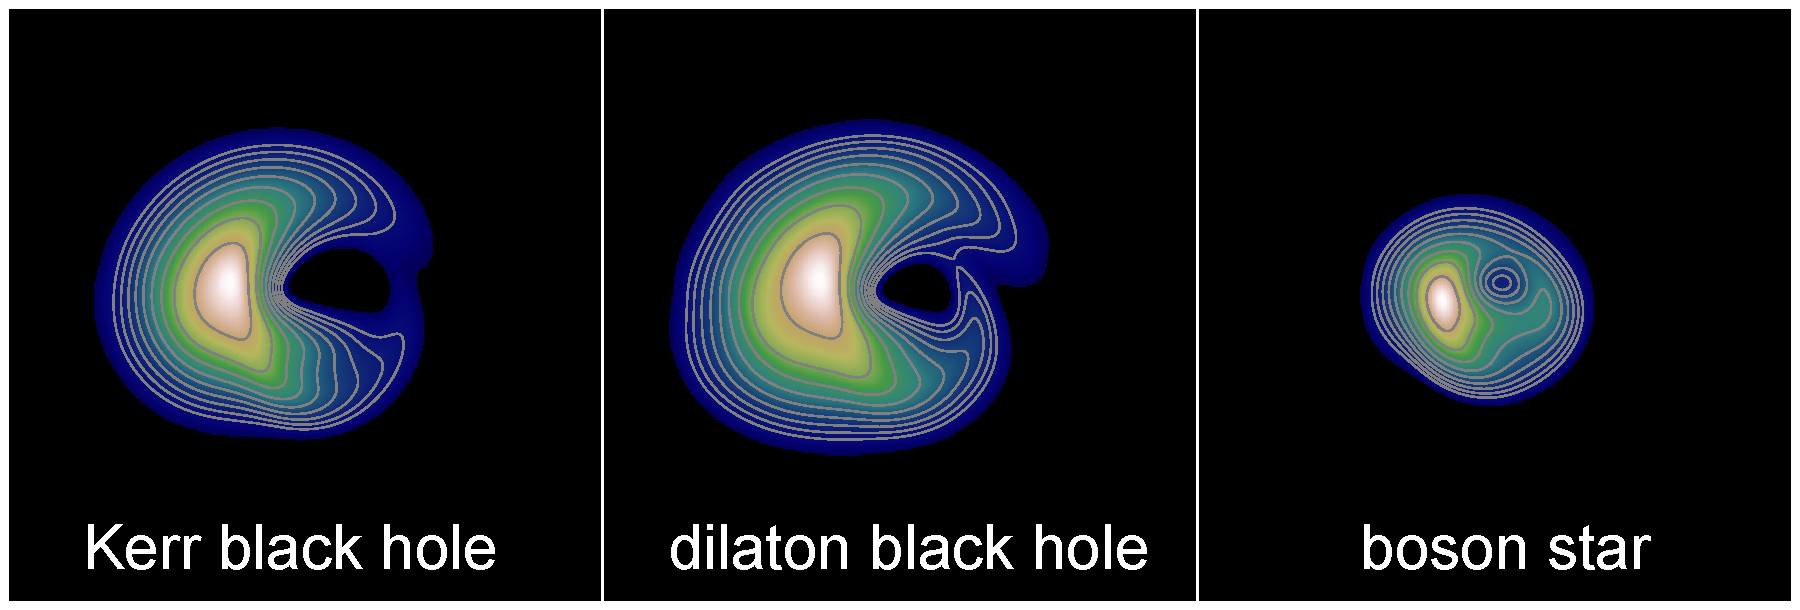
\includegraphics[width=0.88\linewidth,height=0.48\textheight,keepaspectratio]{../figs/pdf/en/fig-07-15.pdf}

% DOCX paragraph 1116
\caption{\emph{Comparación de las imágenes a 230 GHz de tres objetos compactos con la misma masa y sometidos a los mismos procesos de acreción. De izquierda a derecha: un agujero negro de Kerr\index{agujero negro!Kerr}, un agujero negro dilatónico y una estrella de bosones\index{estrella de bosones}. © C. Fromm/Y. Mizuno/H. Olivares/Z. Younsi/LR.}}\label{fig:07-15}
\end{figure}

% DOCX paragraph 1118
Lo bonito de la figura \ref{fig:07-15} es que no requiere mucha explicación. Está bastante claro que, si bien se aprecian diferencias entre cualquiera de los agujeros negros, en los paneles izquierdo y central, y la estrella de bosones\index{estrella de bosones}, en el derecho, no ocurre lo mismo al comparar los dos agujeros negros. En esencia, nuestra investigación nos ha llevado a concluir que hoy es posible distinguir un agujero negro de una estrella de bosones. Esta presenta una sombra\index{sombra (agujero negro)} mucho menor que la de un agujero negro de la misma masa; cabe esperar un comportamiento similar de un agujero de gusano: una sombra más pequeña para la misma masa. Además, dadas las restricciones bastante estrictas sobre la masa de M87*\index{M87*}, que no permiten que el tamaño de la sombra medida varíe demasiado, puede descartarse que una estrella de bosones, al menos en el modelo considerado hasta ahora, sea compatible con la imagen del EHT. Al mismo tiempo, con la calidad actual de la imagen de M87*, no es posible distinguir con suficiente certeza un agujero negro de Kerr\index{agujero negro!Kerr} de uno dilatónico, aunque sus imágenes difieran ligeramente. Eso explica por qué este capítulo se titula «La primera imagen de un agujero negro» y no «La primera imagen de un agujero negro einsteiniano». Por ahora no podemos distinguir un agujero negro de Einstein de otro de una teoría dilatónica, y probablemente tampoco de los que predicen muchas otras teorías.

% DOCX paragraph 1119
Es posible, y quizá incluso probable, que estas conclusiones sigan siendo válidas hasta que se realicen observaciones VLBI con una resolución mucho mayor. Sin embargo, también es muy probable que las observaciones nuevas y repetidas previstas para los próximos años permitan superar algunas de las degeneraciones de la figura \ref{fig:07-14}. Las simulaciones muestran con claridad que la variabilidad\index{variabilidad} de la tasa de acreción es distinta en los diferentes agujeros negros, por lo que comparar imágenes tomadas en distintos momentos puede ser decisivo para romper la degeneración\index{degeneración!interpretación} que ahora aparece al comparar solo dos imágenes estáticas. Una vez más, las imágenes obtenidas hasta ahora de M87*\index{M87*} deben considerarse simplemente las primeras; quedan muchas preguntas que podrán responderse a medida que se realicen nuevas mediciones.

% DOCX paragraph 1120
Quiero terminar este capítulo, dedicado a la primera imagen de un agujero negro, con una consideración general. Ya hemos mencionado que las observaciones del EHT han supuesto una revolución tecnológica y han enriquecido enormemente nuestra comprensión de la astrofísica y de la física gravitatoria. En particular, hay al menos dos resultados científicos de esas observaciones y de su interpretación teórica que se reconocen unánimemente como los más relevantes. El primero es que han aportado pruebas, más allá de toda duda razonable, de que en el centro de la galaxia M87 hay un agujero negro supermasivo en acreción. Puesto que M87 no es una galaxia de características peculiares, estas observaciones nos dicen, por inducción, que toda galaxia debería tener un agujero negro supermasivo en su centro. Es una hipótesis tan antigua como las primeras observaciones de galaxias y agujeros negros, y resulta llamativo que no se confirmara hasta 2019. Quizá aún más importante sea que su confirmación resulta esencial para nuestra comprensión actual de la formación de las estructuras a gran escala del universo.

% DOCX paragraph 1121
La segunda contribución universalmente reconocida de las observaciones del EHT es que han aportado pruebas de una propiedad esencial de la solución de agujero negro en la relatividad general: ¡su simplicidad! Es extraordinario que un objeto como M87*\index{M87*}, con una masa de varios miles de millones de masas solares, tenga exactamente las mismas propiedades que otro de masa cien millones de veces menor, como los agujeros negros revelados por los detectores\index{ondas gravitatorias!detectores} de ondas gravitatorias LIGO\index{LIGO}/Virgo\index{Virgo}. La sencilla posibilidad de reescalar con la masa el comportamiento de los agujeros negros, que hemos encontrado al hablar del teorema de ausencia de pelo, es una predicción precisa de la relatividad general. Las observaciones del EHT y de LIGO/Virgo se complementan de una forma hermosa: ambas son necesarias para explorar el concepto de agujero negro en las escalas mayores y menores en las que se espera que existan.

% DOCX paragraph 1122
Añadiría una última consideración que refleja un punto de vista muy personal: la relevancia más profunda de las observaciones del EHT hay que buscarla en otro lugar. Lo que encuentro más valioso de la primera imagen de un agujero negro es que ha transformado el horizonte de sucesos\index{horizonte de sucesos} de «concepto matemático» en «objeto físico». En otras palabras, las observaciones han mostrado que ahora es posible realizar pruebas experimentales sobre lo que antes era solo un concepto y, como tal, estaba sujeto a opiniones diversas. Parafraseando a Galileo, estas observaciones y todas las que vendrán nos permiten, en esencia, dejar de «[discutir] sobre las mayores cuestiones sin obtener ninguna verdad». Ahora podemos utilizar observaciones reales para comparar teorías diferentes e igualmente plausibles, aceptar las compatibles con las observaciones y rechazar las que no lo son. Hasta ahora se nos había negado la posibilidad de dar este paso trivial, pero esencial, del método científico\index{método científico}. Por tanto, las observaciones del EHT nos han proporcionado, en último término, la herramienta más sencilla e importante para un científico: la posibilidad de llegar a verdades. Ahí reconozco el mayor valor de las observaciones de M87*\index{M87*}.
